\section{Abstract Root Systems}


\begin{fluff}
  Much of this section is motivated by \cite[\S18]{tauvel_yu}.
\end{fluff}


% TODO: Add missing symbols in the list of symbols.


\begin{convention}
  In this section all occuring fields are of characteristic zero, unless otherwise specified.
  We denote for every~{\vectorspace{$\kf$}}~$V$ by~$\pair{-,-} \colon V \times V^* \to \kf$ the bilinear evaluation map~$\pair{v, \varphi} = \varphi(v)$.
\end{convention}





\subsection{Review on Reflections}


\begin{recall}
  \label{recalling reflections}
  \leavevmode
  \begin{enumerate}
    \item
      Let~$V$ be a finite dimensional real vector space with inner product~$\inner{-,-}$.
      Then for every linear subspace~$U$ of~$V$ we have
      \[
        V
        =
        U \oplus U^\perp \,.
      \]
      The \defemph{orthogonal reflection}\index{orthogonal reflection}\index{reflection!orthogonal} at~$U$ is the linear map~$s \colon V \to V$ given by
      \[
        s(u + u') = u - u'
      \]
      for all~$u \in U$ and~$u' \in U^\perp$, i.e.\ the unique linear map~$s \colon V \to V$ with~$s(u) = -u$ for every~$u \in U$ and~$s(u') = u'$ for every~$u' \in U^\perp$.
      If~$p \colon V \to V$ denotes the orthogonal projection onto~$U^\perp$, given by~$p(u + u') = u'$ for all~$u \in U$ and~$u' \in U^\perp$, then for every vector~$v \in V$,
      \[
        s(v)
        =
        v - 2 p(v) \,.
      \]
      
      If~$H$ is a hyperplane in~$V$, i.e.\ a linear subspace of codimension~$1$\index{hyperplane}, then the orthogonal complement~$H^\perp$ is {\onedimensional} and thus of the form~$H^\perp = \gen{\alpha}_{\kf}$ for some nonzero vector~$\alpha \in V$.
      The orthogonal projection~$p$ onto~$H^\perp = \gen{\alpha}_{\kf}$ is given by
      \[
        p(v)
        =
        \frac{\inner{v,\alpha}}{\inner{\alpha,\alpha}} \alpha \,.
      \]
      Indeed, if~$v \in H$ then~$\inner{v,\alpha} = 0$ and thus~$p(v) = 0$, and~$p(\alpha) = \alpha$.
      The orthogonal reflection~$s$ at~$H$ is thus given by
      \[
        s(v)
        =
        v - 2 p(v)
        =
        v - 2 \frac{\inner{v,\alpha}}{\inner{v,v}} \alpha \,.
      \]
      This shows how the reflection at~$H$ can be parametrized by~$\alpha$.
      This reflection is therefore often denoted by~$s_\alpha$.
    \item
      Suppose more generally that~$V$ is a finite dimensional vector space over an arbitrary field~$\kf$ and that~$(-,-)$ is a non-degenerate symmetric bilinear form on~$V$.
      Then for any subspace~$U$ of~$V$ the following conditions are equivalent (as seen in \cref{reviewing orthogonals}):
      \begin{equivalenceslist}
        \item
          $V = U \oplus U^\perp$.
        \item
          The restriction~$\restrict{\inner{-,-}}{U}$ is non-degenerate.
        \item
          The restriction~$\restrict{\inner{-,-}}{U^\perp}$ is non-degenerate.
      \end{equivalenceslist}
      If these conditions are satisfied then we can again consider the \defemph{orthogonal reflection}\index{orthogonal reflection}\index{reflection!orthogonal} at the linear subspace~$U$, and describe it using the orthogonal projection onto~$U^\perp$.
      
      If~$H$ is a hyperplane in~$V$ then~$H^{\perp}$ is {\onedimensional} (as~$\dim V = \dim U + \dim U^\perp$) and thus of the form~$H^{\perp} = \gen{\alpha}_\kf$ for some nonzero vector~$\alpha \in V$.
      The restriction~$\restrict{\inner{-,-}}{H^\perp}$ is non-degenerate if and only~$\inner{\alpha, \alpha} \neq 0$.
      If this condition is satisfied then we can consider the orthogonal reflection at~$H$, which is then again given by
      \[
        s_\alpha(v)
        =
        v - 2 \frac{\inner{v,\alpha}}{\inner{\alpha,\alpha}} \alpha \,.
      \]
    \item
      In the above situation a map~$t \colon V \to V$ is an \defemph{isometry}\index{isometry} with respect to~$\inner{-,-}$ if
      \[
        \inner{t(v), t(w)}
        =
        \inner{v,w}
      \]
      for all~$v, w \in V$.
      Then~$t$ is necessarily invertible because~$\inner{-,-}$ is non-degenerate.
      (If~$v \in \ker(t)$ then~$\inner{v,w} = \inner{t(v),t(w)} = 0$ for every~$w \in V$ and thus~$v = 0$.
      This shows that~$t$ is injectiv and thus an isomorphism by the finite-dimensionality of~$V$.)
      
      If~$V = U \oplus U^\perp$ then the reflection~$s$ at~$U$ is such an isometry:
      We can write~$v_1, v_2 \in V$ as~$v_1 = u_1 + u'_1$ and~$v_2 = u_2 + u'_2$ with~$u_1, u_2 \in U$ and~$u'_1, u'_2 \in U^\perp$.
      Then
      \begin{align*}
        \inner{s(v_1), s(v_2)}
        &=
        \inner{s(u_1 + u'_1), s(u_2 + u'_2)}
        \\
        &=
        \inner{-u_1 + u'_1, -u_2 + u'_2}
        \\
        &=
        \inner{u_1, u_2} + \inner{u'_1, u'_2}
        \\
        &=
        \inner{u_1 + u'_1, u_2 + u'_2}
        \\
        &=
        \inner{v_1, v_2} \,.
      \end{align*}
      In particular, if~$\alpha \in V$ with~$\inner{\alpha, \alpha} \neq 0$ then~$s_\alpha$ is an isometry.
      
      If~$V = U \oplus U^\perp$ and~$t \colon V \to V$ is an isometry then
      \[
        V
        =
        t(U)
        \oplus
        t(U^\perp)
        =
        t(U)
        \oplus
        t(U)^\perp
      \]
      where~$t(U^\perp) = t(U)^\perp$ holds because~$t$ is an isometry.
      Indeed, every~$v \in V$ can be uniquely written as~$v = t(v')$ for some~$v' \in V$, and then
      \begin{align*}
        {}&
        v \in t(U^\perp)
        \\
        \iff{}&
        v' \in U^\perp
        \\
        \iff{}&
        \text{$\inner{v', u'} = 0$ for every~$u' \in U^\perp$}
        \\
        \iff{}&
        \text{$\inner{t(v'), t(u')} = 0$ for every~$u' \in U^\perp$}
        \\
        \iff{}&
        \text{$\inner{v, u''} = 0$ for every~$u'' \in t(U^\perp)$}
        \\
        \iff{}&
        v \in t(U)^\perp \,.
      \end{align*}
      We can now consider both the orthogonal reflection at~$U$, denoted by~$s_U$, and the orthogonal reflection at~$t(U)$, denoted by~$s_{t(U)}$.
      These two reflections are related by the formula
      \[
        s_{t(U)} = t \circ s_U \circ t^{-1} \,.
      \]
      Indeed, the composition~$t \circ s_U \circ t^{-1}$ fixes pointwise the subspace~$t(U)$ and flips the vectors of its orthogonal~$t(U)^\perp = t(U^\perp)$.
      
      If~$\alpha \in V$ is a vector with~$\inner{\alpha, \alpha} \neq 0$ then it follows with~$U = \gen{\alpha}^\perp$ and~$U^\perp = \gen{\alpha}$ that the orthogonal reflections~$s_\alpha$ and~$s_{t(\alpha)}$ are well-defined and related by the formula
      \[
        s_{t(\alpha)}
        =
        t \circ s_\alpha \circ t^{-1} \,.
      \]
  \end{enumerate}
\end{recall}


\begin{definition}
  A \defemph{reflection}\index{reflection} in a~{\vectorspace{$\kf$}}~$V$ is a map~$s \colon V \to V$ with~$s^2 = \id_V$ such that the fixed subspace~$\{v \in V \suchthat s(v) = v\}$ has codimension~one.
\end{definition}


\begin{lemma}[Characterizations of reflections]
  \label{characterizations of reflections}
  Let~$V$ be a~{\vectorspace{$\kf$}} and let~$s \colon V \to V$ be a linear map.
  The following conditions on~$s$ are equivalent:
  \begin{equivalenceslist}
    \item
      \label{is a reflection}
      The map~$s$ is a reflection.
    \item
      \label{is suitable diagonalizable}
      The map~$s$ is diagonalizable with~$V = V_+ \oplus V_-$ where the eigenspace~$V_+ = \{v \in V \suchthat s(v) = v\}$ has codimension~one and the eigenspace~$V_- = \{v \in V \suchthat s(v) = -v\}$ is {\onedimensional}.
    \item
      \label{existence of dual check}
      There exist a vector~$\alpha \in V$ and a linear functional~$\check*{\alpha} \in V^*$ with~$\pair{\alpha, \check{\alpha}} = 2$ such that
      \[
        s(v)
        =
        v - \pair{v, \check{\alpha}} \alpha
      \]
      for every~$v \in V$.
    \item
      \label{maps all vectors into lines}
      There exists some nonzero vector~$\alpha \in V$ with~$s(\alpha) = -\alpha$ such that~$s(v) \in v + \kf \alpha$ for every~$v \in V$.
    \item
      \label{maps generators into lines}
      There exists some nonzero vector~$\alpha \in V$ with~$s(\alpha) = -\alpha$ such that~$s(\beta) \in \beta + \kf \alpha$ for every~$\beta \in R$ where~$R$ is some vector space generating set of~$R$.
  \end{equivalenceslist}
  If these equivalent conditions are satisfies --- i.e.\ if~$s$ is a reflection --- then the eigenspaces~$V_+$ and~$V_-$ of~$s$ depend on the vector~$\alpha$ and the linear functional~$\check{\alpha}$ as~$V_- = \gen{\alpha}_{\kf}$ and~$V_+ = \ker(\check{\alpha})$.
  The characterizations~\ref*{maps all vectors into lines} and~\ref*{maps generators into lines} hold for every nonzero vector~$\alpha \in V_-$.
\end{lemma}


\begin{proof}
  \leavevmode
  \begin{implicationlist}
    \item[\ref*{existence of dual check}~$\implies$~\ref*{is a reflection}]
      We have
      \begin{gather}
        \label{checking flip vector}
        s(\alpha)
        =
        \alpha - \pair{\alpha, \check{\alpha}} \alpha
        =
        \alpha - 2 \alpha
        =
        -\alpha
      \shortintertext{and thus}
        s^2(v)
        =
        s(v - \pair{v, \check{\alpha}} \alpha)
        =
        s(v) - \pair{v, \check{\alpha}} s(\alpha)
        =
        v - \pair{v, \check{\alpha}} \alpha + \pair{v, \check{\alpha}} \alpha
        =
        v
        \notag
      \end{gather}
      for every~$v \in V$.
      This shows~$s^2 = \id_V$.
      It follows from~$\pair{\alpha, \check{\alpha}} = 2$ that~$\alpha \neq 0$ and~$\check{\alpha} \neq 0$.
      Thus
      \begin{equation}
        \label{hyperplane is kernel}
        \{
          v \in V
        \suchthat
          s(v) = v
        \}
        =
        \{
          v \in V
        \suchthat
          v - \pair{v, \check{\alpha}} \alpha = v
        \}
        =
        \{
          v \in V
        \suchthat
          \pair{v, \check{\alpha}} = 0
        \}
        =
        \ker(\check{\alpha})
      \end{equation}
      has codimension~one.

    \item[\ref*{is a reflection}~$\implies$~\ref*{is suitable diagonalizable}]
      The endomorphism~$s$ satisfies the polynomial~$x^2 - 1 = (x-1)(x+1)$ and is therefore diagonalizable with possible eigenvalues~$1$ and~$-1$.
      Thus~$V = V_+ \oplus V_-$.
      The space~$V_+$ has codimension~one because~$s$ is a reflection, so~$V_-$ must be {\onedimensional}.
    \item[\ref*{is suitable diagonalizable}~$\implies$~\ref*{existence of dual check}]
      Let~$\alpha \in V_-$ be nonzero.
      Then~$V = V_+ \oplus \gen{\alpha}_{\kf}$ and there hence exists a unique linear functional~$\check*{\alpha} \in V^*$ with~$\restrict{\check{\alpha}}{V_+} = 0$ and~$\pair{\alpha, \check{\alpha}} = 2$.
      For the resulting linear map
      \begin{gather*}
        s_{\alpha, \check{\alpha}}
        \colon
        V
        \to
        V \,,
        \quad
        v
        \mapsto
        v - \pair{v, \check{\alpha}} \alpha
      \shortintertext{we have}
        s_{\alpha, \check{\alpha}}(v)
        =
        v - \pair{v, \check{\alpha}} \alpha
        =
        v - 0 \cdot \alpha
        =
        v
        =
        s(v)
      \shortintertext{for every~$v \in V_+$ and}
        s_{\alpha, \check{\alpha}}(\alpha)
        =
        \alpha - \pair{\alpha, \check{\alpha}} \alpha
        =
        \alpha - 2 \alpha
        =
        -\alpha
        =
        s(\alpha) \,.
      \end{gather*}
      Thus~$s = s_{\alpha, \check{\alpha}}$ since~$V = V_+ \oplus \gen{\alpha}_{\kf}$.
    \item[\ref*{existence of dual check}~$\implies$~\ref*{maps all vectors into lines}]
      It holds that~$s(v) = v - \pair{v, \check{\alpha}} \alpha \in v + \kf \alpha$ for every vector~$v \in V$ and the conditions~$s(\alpha) = -\alpha$ and~$\pair{\alpha, \check{\alpha}} = 2$ are equivalent.
      It also follows from~$\pair{\alpha, \check{\alpha}} = 2$ that~$\alpha$ is nonzero.
    \item[\ref*{maps all vectors into lines}~$\implies$~\ref*{existence of dual check}]
      There exists for every vector~$v \in V$ some scalar~$\check{\alpha}(v) \in \kf$ with~$s(v) = v + \check{\alpha}(v) \alpha$.
      The given linearity of~$s$ is equivalent to the resulting linearity of the map~$\check{\alpha} \colon V \to \kf$ since~$\alpha$ is nonzero.
      The condition~$s(\alpha) = -\alpha$ is equivalent to the condition~$\pair{\alpha, \check{\alpha}} = 2$.
    \item[\ref*{maps all vectors into lines}~$\iff$~\ref*{maps generators into lines}]
      This holds because~$s$ is~{\linear{$\kf$}} and~$R$ is a generating set for~$R$.
  \end{implicationlist}
  That~$V_+ = \ker(\check{\alpha})$ was shown in~\eqref{hyperplane is kernel} and that~$V_- = \gen{\alpha}_{\kf}$ follows from~\eqref{checking flip vector}.
  We have seen in the proof of the implicaiton~\ref*{is suitable diagonalizable}~$\implies$~\ref*{existence of dual check} that the characterization~\ref*{maps all vectors into lines} holds for every nonzero vector~$\alpha \in V_-$, and it follows from the proof of the equivalence~\ref*{maps all vectors into lines}~$\iff$~\ref*{maps generators into lines} that characterizations~\ref*{maps all vectors into lines} and~\ref*{maps generators into lines} holds for the same vectors~$\alpha$.
\end{proof}


\begin{definition}
  Let~$V$ be a~{\vectorspace{$\kf$}}.
  For any vector~$\alpha \in V$ and any functional~$\check*{\alpha} \in V^*$ with~$\pair{\alpha, \check{\alpha}} = 2$ the \defemph{associated reflection} is the reflection
  \[
    s_{\alpha, \check{\alpha}}
    \colon
    V
    \to
    V \,,
    \quad
    v
    \mapsto
    v - \pair{v, \check{\alpha}} \alpha \,.
  \]
\end{definition}


\begin{remark}
  \label{regarding general reflections}
  \leavevmode
  \begin{enumerate}
    \item
      \label{uniqueness of reflection parametrization}
      Let~$V$ be~{\vectorspace{$\kf$}} and let~$s \colon V \to V$ be a reflection with associated eigenspace decomposition~$V = V_+ \oplus V_-$ and explicit description~$s = s_{\alpha, \check{\alpha}}$ for some vector~$\alpha \in V$ and linear functional~$\check*{\alpha} \in V^*$ with~$\pair{\alpha, \check{\alpha}} = 2$.
      We see from~$V_- = \gen{\alpha}_{\kf}$ that~$\alpha$ is unique up to nonzero scalar, and we see from~$V_+ = \ker(\check{\alpha})$ that~$\check{\alpha}$ is unique up to nonzero scalar.
      Together with the condition~$\pair{\alpha, \check{\alpha}} = 2$ we see that the pair~$(\alpha, \check{\alpha})$ is unique up to the~{\action{$\kf^{\times}$}} given by~$\lambda.(\alpha, \check{\alpha}) = (\lambda \alpha, \lambda^{-1} \check{\alpha})$.
    \item
      Suppose that~$s \colon V \to V$ is a reflection,~$\alpha \in V$ is a vector and~$\check{\alpha} \in V^*$ is a linear functional, such that these three objects are related by the formula~$s(v) = v - \pair{v, \check{\alpha}} \check{\alpha}$.
      Then each of these three objects is uniquely determined by the other two:
      \begin{itemize}
        \item
          If~$\alpha$ and~$\check{\alpha}$ are fixed then the reflection~$s$ is uniquely determined by the above formula.
        \item
          If~$s$ and~$\alpha$ are fixed then~$V = V_+ \oplus \gen{\alpha}_{\kf}$ and the linear functional~$\check{\alpha}$ is uniquely determined by the conditions~$\restrict{\check{\alpha}}{V_+} = \id_{V_+}$ and~$\check{\alpha}(\alpha) = 2$.
        \item
          If~$s$ and~$\check{\alpha}$ are fixed then~$\alpha$ is determined by the condition~$V_- = \gen{\alpha}_{\kf}$ up to scalar multiple, and the condition~$\pair{\alpha, \check{\alpha}} = 2$ restricts this last degree of freedom.
      \end{itemize}
  \end{enumerate}
\end{remark}


\begin{corollary}
  \label{reflected vector is a linear combination}
  Let~$s$ be a reflection in a vector space~$V$ that flips a nonzero vector~$\alpha$ (i.e.~$s(\alpha) = -\alpha$).
  Then for every vector~$\beta \in V$ the reflected vector~$s(\beta)$ is a linear combination of~$\alpha$ and~$\beta$;
  more precisely,~$s(\beta)$ is contained in the line~$\beta + \kf \alpha$.
\end{corollary}


\begin{proof}
  This follows from characterization~\ref*{maps all vectors into lines} of \cref{characterizations of reflections} since for this characterization~$\alpha$ can be chosen arbitrarily under the restrictions~$\alpha \neq 0$ and~$s(\alpha) = -\alpha$.
\end{proof}


\begin{recall}
  \label{orthogonal eigenspaces for isometries}
  Let~$t$ be an isometry for a symmetric bilinear form~$\inner{-,-}$ on a vector space~$V$.
  For every scalar~$\lambda$ let~$V_\lambda$ denote the resulting eigenspace of~$t$.
  Then the eigenspaces~$V_\lambda$ and~$V_\mu$ are orthogonal with respect to~$\inner{-,-}$ unless~$\mu = \lambda^{-1}$.
  
  Indeed, if~$\mu = 0$ then~$V_\mu = \ker(t) = 0$ because~$t$ is injective.
  For~$\mu \neq 0$ we consider two vectors~$v \in V_\lambda$ and~$w \in V_\mu$ and calculate
  \begin{gather*}
    \mu \cdot \inner{v,w}
    =
    \inner{v, t(w)}
    =
    \inner{t^{-1}(v), w}
    =
    \inner{\lambda^{-1} v, w}
    =
    \lambda^{-1} \cdot \inner{v,w} \,.
  \shortintertext{Then}
    (\lambda^{-1} - \mu) \cdot \inner{v,w} = 0 \,.
  \end{gather*}
  and therefore~$\inner{v,w} = 0$ whenever~$\mu = \lambda^{-1}$.
\end{recall}


\begin{corollary}
  \label{orthogonal reflections are orthogonal reflections}
  Let~$V$ be a~{\vectorspace{$\kf$}} and let~$\inner{-,-}$ be a non-degenerate symmetric bilinear form on~$V$.
  Let~$s$ be a reflection on~$V$ which is an isometry with respect to~$\inner{-,-}$ and let~$\alpha \in V$ be a non-zero vector with~$s(\alpha) = -\alpha$.
  Then~$\inner{\alpha, \alpha} \neq 0$ and the reflection~$s$ is for every~$v \in V$ given by
  \[
    s(v)
    =
    v - 2 \frac{\inner{v, \alpha}}{\inner{\alpha, \alpha}} \alpha \,.
  \]
\end{corollary}


\begin{proof}
  It follows from \cref{orthogonal eigenspaces for isometries} that the eigenspace decomposition~$V = V_+ \oplus V_-$ of~$s$ is an orthogonal decomposition with respect to~$\inner{-,-}$.
  It follows (since~$\inner{-,-}$ is non-degenerate) that~$V_+$ is the orthogonal of~$V_-$ and that~$s$ is the orthogonal reflection at~$V_-$, as discussed in \cref{recalling reflections}.
  We have seen in \cref{recalling reflections} the reflection~$s$ is therefore of the claimed form.
\end{proof}


\begin{lemma}
  \label{subspaces invariant under reflection}
  Let~$V$ be a~{\vectorspace{$\kf$}} and let~$s \colon V \to V$ a reflection.
  Suppose that~$s = s_{\alpha, \check{\alpha}}$ for some vector~$\alpha \in V$ and linear functional~$\check*{\alpha} \in V^*$ with~$\pair{\alpha, \check{\alpha}} = 2$.
  Let~$V = V_+ \oplus V_-$ be the eigenspace decomposition of~$V$ with~$V_{\pm} = \{v \in V \suchthat s(v) = \pm v\}$.
  Then for any linear subspace~$U$ of~$V$ the following conditions are equivalent:
  \begin{equivalenceslist}
    \item
      \label{is reflection invariant}
      The subspace~$U$  is~{\invariant{$s$}} (in the sense that~$s(U) \subseteq U$).
    \item
      \label{contains alpha or is contained in kernel}
      $\alpha \in U$ or~$U \subseteq \ker(\check{\alpha})$.
    \item
      \label{contains minus or is contained in plus}
      $V_- \subseteq U$ or~$U \subseteq V_+$.
  \end{equivalenceslist}
  Hence a linear subspace is~{\invariant{$s$}} if and only if it contains the flipped vector~$\alpha$ or if~$s$ acts trivially on it.
\end{lemma}


\begin{proof}
  We show one more implication then necessary.
  \begin{implicationlist}
    \item[\ref*{is reflection invariant}~$\implies$~\ref*{contains alpha or is contained in kernel}]
      If~$U \subseteq \ker(\check{\alpha})$ then~$s$ atcs non-trivially on~$U$.
      Then there exists some~$\beta \in U$ with~$s(\beta) \neq \beta$.
      Then~$s(\beta) - \beta \in U$ is nonzero with~$s(\beta) - \beta = \pair{\beta, \check{\alpha}} \alpha$.
      We then find~$\alpha \in U$.
    \item[\ref*{contains alpha or is contained in kernel}~$\implies$~\ref*{is reflection invariant}]
      If~$U \subseteq \ker(\check{\alpha})$ then~$s$ acts trivially on~$U$ whence~$U$ is~{\invariant{$s$}}.
      Suppose now that~$\alpha$ is contained in~$U$.
      With respect to the decomposition~$V = \gen{\alpha}_{\kf} \oplus \ker(\check{\alpha})$ we can write every~$u \in U$ as~$u = \lambda \alpha + w$ for some~$\lambda \in \kf$ and~$w \in \ker(\check{\alpha})$.
      Then
      \[
        s(u)
        =
        s(\lambda \alpha + w)
        =
        -\lambda \alpha + w \,.
      \]
      We have~$s(u) - u = -2 \lambda \alpha \in U$ and thus~$s(u) = u + (s(u)-u) \in U$.
    \item[\ref*{is reflection invariant}~$\implies$~\ref*{contains minus or is contained in plus}]
      The~{\invariant{$s$}} subspaces of~$V$ are precisely those of the form~$U = U_+ \oplus U_-$ where~$U_+$ is any linear subspace of~$V_+$ and~$U_-$ is any linear subspace of~$V_-$.
      If~$U_- = 0$ then~$U = U_+$ is contained in~$V_+ = \ker(\check{\alpha})$.
      Otherwise~$\gen{\alpha}_{\kf} = V_-$ is contained in~$U$ whence~$\alpha$ is contained in~$U$.
    \item[\ref*{contains alpha or is contained in kernel}~$\iff$~\ref*{contains minus or is contained in plus}]
      This holds because~$V_- = \gen{\alpha}_{\kf}$ and~$V_+ = \ker(\check{\alpha})$.
    \qedhere
  \end{implicationlist}
\end{proof}


\begin{fluff}
  \label{reflections using duality}
  So far we have described a reflection~$s$ in a finite dimensional~{\vectorspace{$\kf$}}~$V$ by using a vector~$\alpha \in V$ and a linear functional~$\check{\alpha} \in V^*$, so that
  \[
    s(v)
    =
    v - \pair{v, \check{\alpha}} \alpha
  \]
  for all~$v \in V$, where~$\pair{-,-} \colon V \times V^* \to \kf$.
  Then in paritcular~$\pair{\alpha, \check{\alpha}} = 2$, and conversely every choice of~$\alpha \in V$ and~$\check{\alpha} \in V^*$ satisfying this condition defines a reflection.
  
  Suppose not that we are given another finite dimensional~{\vectorspace{$\kf$}}~$W$ and a non-degenerate bilinear pairing~$\pair{-,-} \colon V \times W \to \kf$.
  This non-degenerate pairing corresponds to a vector space isomorphism~$\varphi \colon W \to V^*$ with
  \[
    \pair{v, w}
    =
    \pair{v, \varphi(w)}
  \]
  for every~$w \in W$.
  We can therefore replace the role of the dual space~$V^*$ and its standard pairing~$\pair{-,-} \colon V \times V^* \to \kf$ by that of~$W$ and the non-degenerate bilinear pairing~$\pair{-,-} \colon V \times W \to \kf$.
  
  More specifically, we make the following observations:
  \begin{enumerate}
    \item
      A linear map~$s \colon V \to V$ is a reflection if and only if there exists some vector~$\alpha \in V$ and~$\check{\alpha} \in W$ such that~$s$ is given by~$s(v) = v - \pair{v, \check{\alpha}} \alpha$ for every~$v \in V$.
    \item
      In particular, every choice of vectors~$\alpha \in V$ and~$\check{\alpha} \in V^*$ defines a reflection
      \[
        s_{\alpha, \check{\alpha}}
        \colon
        V
        \to
        V \,,
        \quad
        v
        \mapsto
        v - \pair{v, \check{\alpha}} \alpha \,.
      \]
    \item
      The eigenspaces~$V_+$ and~$V_-$ of~$s$ are given by~$V_+ = (\check{\alpha})^\perp$ and~$V_- = \gen{\alpha}_{\kf}$.
    \item
      The pair~$(\alpha, \check{\alpha})$ is then uniquely determined up to a normalization of the form~$(\lambda \alpha, \lambda^{-1} \check{\alpha})$ with~$\lambda \in \kf^\times$.
    \item
      Of the three objects~$s$,~$\alpha$ and~$\check{\alpha}$ any two of them uniquely determine the third.
    \item
      A linear subspace~$U$ of~$V$ is~{\invariant{$s$}} if and only if~$\alpha \in U$ or~$U \subseteq (\check{\alpha})^\perp$.
  \end{enumerate}
  
  Note that if~$W = V^*$ and~$\pair{-,-}$ is the standard pairing then~$\varphi = \id$ then we regain the original situation that we have previously considered.
  One may think about the non-degenerate bilinear pairing~$\pair{-,-}$ as a \enquote{duality}, and about the standard pairing~$\pair{-,-}$ as the \enquote{standard duality}.
\end{fluff}


\begin{recall}
  \label{recalling the transposed map}
  Let~$f \colon V \to V'$ be a linear map between finite dimensional~{\vectorspaces{$\kf$}} and let~$\pair{-,-} \colon V \times W \to \kf$ and~$\pair{-,-} \colon V' \times W' \to \kf$ be non-degenerate bilinear forms.
  Then there exists a unique linear map~$f^* \colon W' \to W$ with
  \[
    \pair{\spacing f(v), w'}
    =
    \pair{v, \spacing f^*(w')}
  \]
  for all~$v \in V$ and~$w' \in W'$.
  The map~$f^*$ is the \defemph{dual}\index{dual map}\index{map!dual} or \defemph{transpose}\index{transpose map}\index{map!transpose} of~$f$.
  If the map~$f$ is an isomorphism then the induced map~$f^*$ is again an isomorphism and its inverse is given by~$(\spacing f^*)^{-1} = (\spacing f^{-1})^*$.
  We denote this inverse by~$f^{-*}$.
  
  We observe that that
  \[
    f^*(w')^\perp
    =
    f^{-1}\bigl( (w')^\perp \bigr) \,,
  \]
  which an equality of linear subspaces of~$V$.
  Indeed, we find that for every~$v \in V$,
  \begin{align*}
    v \in f^*(w')^\perp
    &\iff
    \pair{v, \spacing f^*(w')} = 0
    \\
    &\iff
    \pair{\spacing f(v), w'} = 0
    \\
    &\iff
    f(v) \in (w')^\perp
    \\
    &\iff
    v \in \spacing f^{-1}\bigl( (w')^\perp \bigr) \,.
  \end{align*}
\end{recall}


\begin{lemma}
  \label{properties of reflections}
  Let~$V$ be a finite dimensional~{\vectorspace{$\kf$}} and let~$\pair{-,-} \colon V \times W \to \kf$ be a non-degenerate bilinear form.
  \begin{enumerate}
    \item
      \label{conjugation of reflection}
      Let~$s \colon V \to V$ be a reflection, given by~$s = s_{\alpha, \check{\alpha}}$ for some vectors~$\alpha \in V$ and~$\check*{\alpha} \in W$.
      Let~$t \colon V \to V$ be any vector space isomorphism.
      Then
      \[
        t \circ s_{\alpha, \check{\alpha}} \circ t^{-1}
        =
        s_{t(\alpha), t^{-*}(\check{\alpha})} \,.
      \]
    \item
      \label{dual reflections}
      Let~$\alpha \in V$ and~$\check{\alpha} \in W$ with~$\pair{\alpha, \check{\alpha}} = 2$.
      Let
      \begin{alignat*}{2}
        s_\alpha
        &\colon
        V
        \to
        V \,,
        &
        \quad
        v
        &\mapsto
        v - \pair{v, \check{\alpha}} \alpha
      \shortintertext{and}
        s_{\check{\alpha}}
        &\colon
        W
        \to
        W \,,
        &
        \quad
        w
        &\mapsto
        w - \pair{\alpha, w} \check{\alpha}
      \end{alignat*}
      be the resulting reflections on~$V$ and~$W$.
  \end{enumerate}
\end{lemma}


\begin{proof}
  \leavevmode
  \begin{enumerate}
    \item
      The reflection~$s_{t(\alpha), t^{-*}(\check{\alpha})}$ is well-defined because
      \[
        \pair{t(\alpha), t^{-*}(\check{\alpha})}
        =
        \pair{t(\alpha), (t^{-1})^*(\check{\alpha})}
        =
        \pair{t^{-1}(t(\alpha)), \check{\alpha}}
        =
        \pair{\alpha, \check{\alpha}}
        =
        2 \,.
      \]
      The vector~$t(\alpha)$ is flipped by the reflection~$s_{t(\alpha), t^{-*}(\check{\alpha})}$ and it is also flipped by the composition~$t \circ s_{\alpha, \check{\alpha}} \circ t^{-1}$ because~$s_{\alpha, \check{\alpha}}$ flips the vector~$\alpha$.
      The fixed hyperplane of the reflection~$s_{t(\alpha), t^{-*}(\check{\alpha})}$ is given by
      \[
        t^{-*}( \check{\alpha} )^\perp
        =
        (t^{-1})^*(\check{\alpha})^\perp
        =
        (t^{-1})^{-1}\bigl( (\check{\alpha})^\perp \bigr)
        =
        t\bigl( (\check{\alpha})^\perp \bigr) \,.
      \]
      (The second equality is explained in \cref{recalling the transposed map}.)
      This hyperplane is also pointwise fixed by the composition~$t \circ s_{\alpha, \check{\alpha}} \circ t^{-1}$ because~$s_{\alpha, \check{\alpha}}$ fixes pointwise the hyperplane~$(\check{\alpha})^\perp$.
      
      This shows that indeed~$t \circ s_{\alpha, \check{\alpha}} \circ t^{-1} = s_{t(\alpha), t^{-*}(\check{\alpha})}$.
    \item
      We have
      \begin{align*}
        \SwapAboveDisplaySkip
        \pair{s_{\alpha}(v), w}
        &=
        \pair[\big]{v - \pair{v, \check{\alpha}} \alpha, w}
        \\
        &=
        \pair{v, w} - \pair{v, \check{\alpha}} \pair{\alpha, w}
        \\
        &=
        \pair[\big]{v, w - \pair{\alpha, w} \check{\alpha}}
        \\
        &=
        \pair{v, s_{\check{\alpha}}(w)}
      \end{align*}
      for all~$v \in V$ and~$w \in W$.
      This shows that the reflection~$s_{\check{\alpha}}$ satisfies the defining property of~$s_\alpha^*$.
    \qedhere
  \end{enumerate}
\end{proof}





\subsection{Definition and First Examples}


\begin{lemma}[Uniqueness of reflections]
  \label{uniqueness of reflections}
  Let~$R$ be a finite generating set of a~{\vectorspace{$\kf$}}~$V$ and let~$s, t \colon V \to V$ be two reflections that leave~$R$ invariant (in the sense that~$s(R) = R$ and~$t(R) = R$) and such that~$s(\alpha), t(\alpha) = -\alpha$ for some nonzero vector~$\alpha \in R$.
  Then~$s = t$.
\end{lemma}


\begin{proof}[First proof]
  We may write both reflections in the form~$s = s_{\alpha, \check{\alpha}}$ and~$t = s_{\alpha, \check{\beta}}$ for some~$\check{\alpha}, \check*{\beta} \in V^*$ with~$\pair{\alpha, \check{\alpha}} = \pair{\alpha, \check{\beta}} = 2$.
  Then
  \begin{align*}
    (t \circ s)(v)
    &=
    t(s(v))
    \\
    &=
    t\bigl( v - \pair{v, \check{\alpha}} \alpha \bigr)
    \\
    &=
    t(v) - \pair{v, \check{\alpha}} t(\alpha)
    \\
    &=
    v - \pair{v, \check{\beta}} \alpha + \pair{v, \check{\alpha}} \alpha
    \\
    &=
    v - \pair{v, \check{\beta} - \check{\alpha}} \alpha \,.
  \end{align*}
  Since~$(t \circ s)(\alpha) = \alpha$ we now find inductively that
  \begin{equation}
    \label{inductive reflection formula}
    (t \circ s)^n(v)
    =
    v - n \pair{v, \check{\beta} - \check{\alpha}} \alpha
  \end{equation}
  for every~$n \geq 0$, because
  \begin{align*}
    (t \circ s)^{n+1}(v)
    &=
    (t \circ s)((t \circ s)^n(v))
    \\
    &=
    (t \circ s)(v - n \pair{v, \check{\beta} - \check{\alpha}} \alpha)
    \\
    &=
    (t \circ s)(v) - n \pair{v, \check{\beta} - \check{\alpha}} (t \circ s)(\alpha)
    \\
    &=
    v - \pair{v, \check{\beta} - \check{\alpha}} \alpha - n \pair{v, \check{\beta} - \check{\alpha}} \alpha
    \\
    &=
    v - (n+1) \pair{v, \check{\beta} - \check{\alpha}} \alpha \,.
  \end{align*}

  
  The restriction of~$t \circ s$ to~$R$ is a permuation of~$R$, which is a finite set.
  There hence exists some power~$n \geq 1$ with~$\restrict{(t \circ s)^n}{R} = \id_{R}$.
  Then already~$(t \circ s)^n = \id_V$ since~$V$ is spanned by~$R$.
  It follows from the formula~\eqref{inductive reflection formula} (and~$\ringchar(\kf) = 0$,~$\alpha \neq 0$) that~$\pair{v, \check{\beta} - \check{\alpha}} = 0$ for every~$v \in V$.
  Thus~$\check{\beta} - \check{\alpha} = 0$ and therefore~$\check{\alpha} = \check{\beta}$.
  This shows that indeed~$s = s_{\alpha, \check{\alpha}} = s_{\alpha, \check{\beta}} = t$.
\end{proof}


\begin{proof}[Second proof({\cite[3.7.3.1.4]{winter}})]
  Let~$G$ be the subgroup of~$\GL(V)$ generated by~$s$ and~$t$.
  We may identify~$G$ with a subgroup of the symmetric group of the finite set~$R$ since the reflections~$s$ and~$t$ satisfy~$s(R) = t(R) = R$ and~$V$ is generated by~$R$.
  It follows that~$G$ is finite.
  
  The line~$L \defined \gen{\alpha}_{\kf}$ is a {\onedimensional}~{\subrepresentation{$G$}} of~$V$.
  It follows from Maschke’s theorem that there exists a~{\subrepresentation{$G$}}~$W$ of~$V$ with~$V = L \oplus W$.
  (To apply Maschke’s theorem we use that~$G$ is finite and that~$\ringchar(\kf) = 0$.)
  It follows from \cref{subspaces invariant under reflection} that~$s$ and~$t$ act trivially on~$W$.
  So
  \[
    \restrict{s}{L}
    =
    - \id_L
    =
    \restrict{t}{L}
    \quad\text{and}\quad
    \restrict{s}{W}
    =
    \id_W
    =
    \restrict{t}{W} \,.
  \]
  and therefore~$s = t$.
\end{proof}


\begin{example}[Motivation]
  Let~$\glie$ be a finite dimensional semisimple Lie~algebra over an algebraically closed field~$\kf$ of characteristic zero.
  Let~$\hlie$ be a Cartan~subalgebra of~$\glie$ and let~$R \defined \Phi(\glie, \hlie)$ be the associated set of roots, which is a subset of~$\hlie^*$.
  For every~$\alpha \in R$ let~$h_\alpha \in \hlie$ as explained in \cref{construction of S alpha}.
  Every element~$h_\alpha$ defines an element~$\check*{\alpha} \in \hlie^{**}$ that is given by evaluation at~$h_\alpha$, and thus a reflection
  \[
    s_\alpha
    \colon
    \hlie^*
    \to
    \hlie^* \,,
    \quad
    \varphi
    \mapsto
    \varphi - \pair{\varphi, \check{\alpha}} \alpha
    =
    \varphi - \pair{\alpha, \varphi} \alpha \,.
  \]
  We have previously made the following observations:
  \begin{itemize}
    \item
      The set~$R$ does not contain~$0$ (by definition) and is finite (because~$\glie$ is finite dimensional).
    \item
      The set~$R$ spans~$\hlie^*$ (by \cref{basics properties of roots}).
    \item
      For every~$\alpha \in R$ the multiples of~$\alpha$ that are again contained in~$R$ are precisely~$\alpha$ and~$-\alpha$ (by \cref{roots spaces are onedimensional and reduced}).
    \item
      We have~$s_\alpha(\beta) \in \beta + \Integer \alpha$ for all~$\alpha, \beta \in R$ (by \cref{integral and reflection properties of root pairing}).
    \item
      We have~$s_{\alpha, \check{\alpha}}(\beta) \in R$ for all~$\alpha, \beta \in R$ (by \cref{integral and reflection properties of root pairing}).
  \end{itemize}
  Motivated by this example we make the following definition:
\end{example}


\begin{definition}
  Let~$V$ be a~{\vectorspace{$\kf$}}.
  A subset~$R$ of~$V$ is an \defemph{abstract root system}\index{abstract!root system}\index{root system!abstract}, or simply \defemph{root system}\index{root system} if it satisfies the following conditions:
  \begin{enumerate}[label = (R\arabic*), start=0]
    \item
      \label{does not contain zero}
      The set~$R$ does not contain the zero vector.
    \item
      \label{root system spans}
      The vector space~$V$ is spanned by~$R$.
    \item
      \label{closed under reflections}
      For every element~$\alpha$ there exists a reflection~$s_\alpha$ of~$V$ with~$s_\alpha(\alpha) = -\alpha$ such that~$s_\alpha(R) \subseteq R$.
  \end{enumerate}
  The root system~$R$ is \defemph{reduced}\index{reduced root system}\index{root system!reduced} if
  \begin{enumerate}[label = (R\arabic*), resume]
    \item
      for every~$\alpha \in R$ the only multiples of~$\alpha$ that are again contained in~$R$ are~$\alpha$ and~$-\alpha$.
  \end{enumerate}
  The root system~$R$ is \defemph{crystallographic}\index{crystallographic root system}\index{root system!crystallographic} if
  \begin{enumerate}[label = (R\arabic*), resume]
    \item
      $s_\alpha(\beta) \in \beta + \Integer \alpha$ for all~$\alpha, \beta \in R$.
  \end{enumerate}
%   The elements of~$R$ are the \defemph{roots}\index{root}, and the \defemph{coroots}\index{coroot}\index{root system!coroot} are the elements of the set
%   \[
%     \check{R}
%     \defined
%     \{
%       \check{\alpha}
%     \suchthat
%       \alpha \in R
%     \} \,.
%   \]
  The elements of~$R$ are the \defemph{roots}\index{root} of~$R$.
  The \defemph{rank}\index{rank}\index{root system!rank} of the root system~$R$ is the dimension of~$V$, i.e.\ the dimension of the span of~$R$.
  A root system~$R$ in a~{\vectorspace{$\kf$}}~$V$ will sometimes be denoted as a pair~$(R, V)$.
\end{definition}


\begin{remark}
  \leavevmode
  \begin{enumerate}
    \item
      If~$R$ is a root system in a~{\vectorspace{$\kf$}}~$V$ then~$V$ is necessarily finite dimensional since~$V$ is spanned by the finite set~$R$.
    \item
      Condition~\ref*{root system spans} in the definition of a root system is given for technical reasons, and in a certain sense not essential:
      
      We require condition~\ref*{root system spans} simply so that we can apply \cref{uniqueness of reflections}.
      By doing so we find that for every root~$\alpha \in R$ the reflection~$s_\alpha$ is unique.
      A root system in vector space~$V$ is therefore completely determined by the corresponding subset~$R$ of~$V$.
      
      To see how the condition~\ref*{root system spans} is not essential, let~$R$ be a subset of a~$V$ satisfying the conditions~\ref*{does not contain zero} and~\ref*{closed under reflections}.
      By condition~\ref*{closed under reflections} the span of~$R$, that we denote by~$V'$, is~{\invariant{$s_\alpha$}} for every~$\alpha \in R$.
      We can therefore restrict the reflections~$s_\alpha$ to an endomorphisms~$V'$.
      Then~$s'_\alpha(\alpha) = -\alpha$ and~$s'_\alpha(R) \subseteq R$.
      This means that~$R$ is again a root system --- just not in~$V$, but in~$V'$.
      
      So if we leave out conditon~\ref*{root system spans} then we lose the uniqueness of the reflections~$s_\alpha$, but don’t really gain any new kind of root systems.
      We have therefore decided to require~\ref*{root system spans} in our definition.
    \item
      We have for every root~$\alpha \in R$ that~$-\alpha = s_\alpha(\alpha) \in R$.
      That~$R$ is reduced is therefore only a restriction on which multiples of~$\alpha$ are allowed to be contained in~$R$, but make no additional requirement on which multiples of~$\alpha$ are required to appear in~$R$.
%    \item
%      To motivate the term \enquote{crystallographic} let~$R$ be a root system in a vector space~$V$.
%      Let~$L$ be the abelian subgroup of~$V$ generated by~$R$.
%      Then~$L$ is a finitely generated abelian group, and it is torsion-free because~$V$ is torsion free (since~$\ringchar(\kf) = 0$).
%      It follows from the classification of finitely generated abelian groups that~$L$ is a free abelian group.
%      This means that~$L$ is a lattice in~$R$.
%      If the root system~$R$ is crystallographic then this is invariant under the reflections~$s_\alpha$ with~$\alpha \in R$, since ~$s_\alpha(\beta) \in \beta + \Integer \alpha \subseteq L$ for all~$\alpha, \beta \in R$, and thus
%      \[
%        s_\alpha(L)
%        =
%        s_\alpha\left( \sum_{\beta \in R} \Integer \beta \right)
%        =
%        \sum_{\beta \in R} \Integer s_\alpha(\beta)
%        \subseteq
%        \sum_{\beta \in R} L
%        =
%        L \,.
%      \]
%      
%      The converse does (sadly) not hold:
%      It may happen that~$s_\alpha(L) = L$ for every~$\alpha \in R$ even though~$R$ is not crystallographic.
%      One can take for example~$V = \kf$ and~$R = \{-3, -2, 2, 3\}$.
%      Then the reflection~$s_\alpha$ is for every~$\alpha \in R$ (necessarily) given by~$s_\alpha(x) = -x$.
%      Thus~$L$ is~{\invariant{$s_\alpha$}} for every~$\alpha \in R$.
%      But~$s_3(2) = -2 \notin 2 + 3 \Integer$.
%      
%      We note that the condition~$s_\alpha(\beta) \in \beta + \Integer \alpha$ is always satisfied for~$\beta = \pm \alpha$ since
%      \[
%        s_\alpha(\pm \alpha)
%        =
%        \mp \alpha
%        =
%        \pm \alpha \mp 2 \alpha
%        \in
%        \pm \alpha + \Integer \alpha \,.
%      \]
%      To examine if a root system is crystallographic we therefore only need to look at the possibilities for~$\beta \neq \pm \alpha$ in more detail.
    \item
      For the study of semisimple Lie~algebras we will be interested in root systems that are both reduced and crystallographic.
      But at least for now we will not assume these conditions.
  \end{enumerate}
\end{remark}


\begin{example}[Root systems of rank~zero]
  The empty root system~$\emptyset$ is the unique root system of rank~$0$, i.e.\ the unique root system that is admitted by the zero vector space.
  This root system is both reduced and crystallograpic.
\end{example}


\begin{example}[Root systems of rank~one]
  Let~$V$ be a {\onedimensional} vector space.
  Note that~$V$ admits only one reflection, namely~$s(x) = -x$, since necessarily~$V_- = V$.
  \begin{enumerate}
    \item
      The root systems in~$V$ are precisely those subsets of the form~$R = \{ \pm \alpha_1, \dotsc, \pm \alpha_n \}$ where~$\alpha_1, \dotsc, \alpha_n$ are nonzero and~$n \geq 1$.
      \begin{center}
        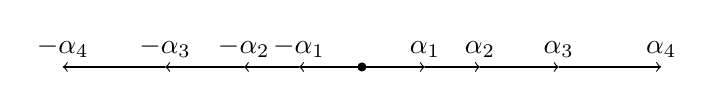
\begin{tikzpicture}
          % center point
          \draw[fill] (0,0) circle (0.05);
          % positive roots
          \draw[->] (0,0) -- (0.8,0) node[above]{$\alpha_1$};
          \draw[->] (0.8,0) -- (1.5,0) node[above]{$\alpha_2$};
          \draw[->] (1.5,0) -- (2.5,0) node[above]{$\alpha_3$};
          \draw[->] (2.5,0) -- (3.8,0) node[above]{$\alpha_4$};
          % negative roots
          \draw[->] (0,0) -- (-0.8,0) node[above]{$-\alpha_1$};
          \draw[->] (-0.8,0) -- (-1.5,0) node[above]{$-\alpha_2$};
          \draw[->] (-1.5,0) -- (-2.5,0) node[above]{$-\alpha_3$};
          \draw[->] (-2.5,0) -- (-3.8,0) node[above]{$-\alpha_4$};
        \end{tikzpicture}
      \end{center}
    \item
      A root system in~$V$ is reduced if and only if it is of the form~$R = \{\alpha, -\alpha\}$ for some nonzero~$\alpha \in V$.
      \begin{center}
        \begin{tikzpicture}
          % center point
          \draw[fill] (0,0) circle (0.05);
          % roots
          \draw[->] (0,0) -- (2,0) node[right]{$\alpha$};
          \draw[->] (0,0) -- (-2,0) node[left]{$-\alpha$};
        \end{tikzpicture}
      \end{center}
    \item
      A root system in~$V$ is crystallographic if and only if it is of the form~$R = \{\alpha, -\alpha\}$ for some nonzero~$\alpha \in V$ or of the form~$R = \{\alpha, 2\alpha, -\alpha, -2\alpha\}$ for some nonzero~$\alpha \in V$.
      \begin{center}
        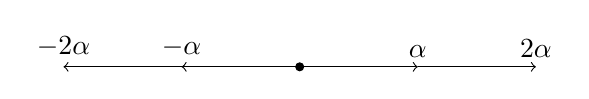
\begin{tikzpicture}
          % center point
          \draw[fill] (0,0) circle (0.05);
          % roots
          \draw[->] (0,0) -- (1.5,0) node[above]{$\alpha$};
          \draw[->] (1.5,0) -- (3,0) node[above]{$2\alpha$};
          \draw[->] (0,0) -- (-1.5,0) node[above]{$-\alpha$};
          \draw[->] (-1.5,0) -- (-3,0) node[above]{$-2\alpha$};
        \end{tikzpicture}
      \end{center}
      
      Indeed, if~$R = \{\alpha, -\alpha\}$ then~$R$ is crystallographic, and if~$R = \{\alpha, -\alpha, 2\alpha, -2\alpha\}$ then we also find that~$s(2\alpha) = 2s(\alpha) \in 2(\alpha + \Integer \alpha) \subseteq 2\alpha + \Integer$.
      
      Suppose now conversely that~$R$ is any crystallographic root system in~$V$.
      Then~$R$ contains some nonzero vector~$\alpha$.
      If~$\beta \in R$ is any other root then~$\beta = \lambda \alpha$ for some nonzero scalar~$\lambda$.
      Then
      \[
        \Integer \alpha
        \ni
        s(\beta) - \beta
        =
        -2 \beta
        =
        -2 \lambda \alpha
      \]
      and thus~$-2 \lambda \in \Integer$, i.e.~$\lambda \in 2^{-1} \Integer$.
      By switching the roles of~$\alpha$ and~$\beta$ we find in the same way that also~$\lambda^{-1} \in 2^{-1} \Integer$.
      We have found that~$\lambda$ is a nonzero half-integer whose inverse~$\lambda^{-1}$ is again a half-integer.
      This leaves for~$\lambda$ only the choices~$\pm 1$,~$\pm 2$ and~$\pm 1/2$, which proves the assertion.
  \end{enumerate}
  
  The above argument shows more generally that if~$R$ is a crystallographic root system in any vector space~$V$, then for every root~$\alpha \in R$ the only multiples of~$R$ that can again be roots are~$\pm \alpha$,~$\pm 2 \alpha$ and~$\pm \alpha/2$.
\end{example}


\begin{examples}[Root system in~$\Real^n$]
  \label{root systems in Rn}
  Suppose that~$V$ is a real vector space with inner product~$\inner{-,-}$.
  Then we denote for every nonzero vector~$\alpha \in V$ by
  \[
    H_\alpha
    \defined
    \{
      v \in V
    \suchthat
      \inner{v,\alpha}
      =
      0
    \}
  \]
  the hyperplane orthogonal to~$\alpha$ and by~$s_\alpha \colon V \to V$ the reflection at~$H_\alpha$, as explained in \cref{recalling reflections}.
  Observe that for~$V = \Real^n$ we have the following special reflections:
  \begin{itemize}
    \item
      The reflection~$s_{e_i}$ is given by~$s_{e_i}(e_i) = -e_i$ and~$s_{e_i}(e_j) = e_j$ for~$j \neq i$.
      This means that this reflection flips the sign of the~{\howmanyth{$i$}} standard basis vector.
    \item
      To calculate the reflection~$s_{e_i - e_j}$ we observe that
      \[
        H_\alpha
        =
        \gen{
          e_i + e_j,
          e_1
          \dotsc,
          \widehat{e_i},
          \dotsc,
          \widehat{e_j},
          \dotsc,
          e_n
        }_{\Real}
      \]
      since this linear subspace is orthogonal to~$e_i - e_j$ and of the right dimension (namely~$n-1$).
      It follows that~$s_{e_i-e_j}(e_k) = e_k$ for~$k \neq i,j$.
      We also find
      \[
        s_{e_i-e_j}(e_i)
        =
        s_{e_i-e_j}\left( \frac{e_i - e_j}{2} + \frac{e_i + e_j}{2} \right)
        =
        -\frac{e_i - e_j}{2} + \frac{e_i + e_j}{2}
        =
        e_j
      \]
      and therefore also~$s_{e_i-e_j}(e_j) = e_i$.
      This shows that the reflection~$s_{e_i-e_j}$ swaps the two standard basis vectors~$e_i+e_j$.
    \item
      The reflections~$s_{e_i}$ is an isometry, and therefore
      \[
        s_{e_i + e_j}
        =
        s_{s_{e_j}(e_i - e_j)}
        =
        s_{e_j} \circ s_{e_i - e_j} \circ s_{e_j}^{-1}
        =
        s_{e_j} \circ s_{e_i - e_j} \circ s_{e_j}
      \]
      as seen in \cref{recalling reflections}.
      We find from the above explicit descriptions of the reflections~$s_{e_i}$ and~$s_{e_i - e_j}$ that the reflection~$s_{e_i + e_j}$ fixes the standard basis vectors~$e_k$ with~$k \neq i,j$ and is given on the other two standard basis vectors by~$s_{e_i + e_j}(e_i) = -e_j$ and~$s_{e_i + e_j}(e_j) = -e_i$.
  \end{itemize}
  
  We now use the above calculations to give examples of root systems~$R$ in (a suitable linear subspace of)~$\Real^n$ for which the reflection~$s_\alpha$ for~$\alpha \in R$ is the orthogonal reflection at the hyperplane~$H_\alpha$ as above.
  This means that
  \[
    s_\alpha(x)
    =
    x - 2 \frac{(x,\alpha)}{\norm{\alpha}^2} \alpha \,,
  \]
  as explained in \cref{recalling reflections}.
  Any such constructed root system~$R$ will therefore be crystallographic if and only if~$2 (\alpha,\beta)/\norm{\alpha}^2 \in \Integer$ for all~$\alpha, \beta \in R$.

  
  \begin{enumerate}
    \item
      The set~$R = \{ \pm e_i \suchthat i = 1, \dotsc, n\}$ is a reduced, crystallographic root system in~$\Real^n$.
      
      The set~$R$ spans~$\Real^n$ and does not contain the zero vector, and the reflections~$s_{\pm e_i} = s_{e_i}$ flip the standard basis vector~$e_i$, so that~$s_{e_i}(R) \subseteq R$.
      This shows that~$R$ is a root system, and we see (directly) that it is reduced.
      It is crystallographic since
      \[
        2 \frac{(e_i, e_j)}{\norm{e_i}^2}
        =
        2 \delta_{ij}
        \in
        \Integer
      \]
      for all~$i, j = 1, \dotsc, n$.
      
      For small values of~$n$ these root systems looks as follows:
      \begin{center}
        \begingroup
        \setlength{\tabcolsep}{18pt} %normal 6pt
        \begin{tabular}{ccc}
          \begin{tikzpicture}
            % center point
            \draw[fill] (0,0) circle (0.05);
            % roots
            \draw[->] (0,0) -- (1,0);
            \draw[->] (0,0) -- (-1,0);
            \draw[opacity=0] (0,0) -- (0,1);
            \draw[opacity=0] (0,0) -- (0,-1);
          \end{tikzpicture}
          &
          \begin{tikzpicture}
            % roots
            \draw[->] (0,0) -- (1,0);
            \draw[->] (0,0) -- (-1,0);
            \draw[->] (0,0) -- (0,1);
            \draw[->] (0,0) -- (0,-1);
          \end{tikzpicture}
          &
          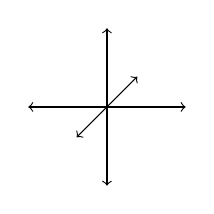
\begin{tikzpicture}
            % roots
            \draw[->] (0,0,0) -- (1,0,0);
            \draw[->] (0,0,0) -- (-1,0,0);
            \draw[->] (0,0,0) -- (0,1,0);
            \draw[->] (0,0,0) -- (0,-1,0);
            \draw[->] (0,0,0) -- (0,0,1);
            \draw[->] (0,0,0) -- (0,0,-1);
%             % cube
%             \draw[dashed] (1,1,1) -- (1,1,-1);
%             \draw[dashed] (1,-1,1) -- (1,-1,-1);
%             \draw[dashed] (-1,1,1) -- (-1,1,-1);
%             \draw[dashed] (-1,-1,1) -- (-1,-1,-1);
%             \draw[dashed] (1,1,1) -- (1,-1,1);
%             \draw[dashed] (1,1,-1) -- (1,-1,-1);
%             \draw[dashed] (-1,1,1) -- (-1,-1,1);
%             \draw[dashed] (-1,1,-1) -- (-1,-1,-1);
%             \draw[dashed] (1,1,1) -- (-1,1,1);
%             \draw[dashed] (1,-1,1) -- (-1,-1,1);
%             \draw[dashed] (1,1,-1) -- (-1,1,-1);
%             \draw[dashed] (1,-1,-1) -- (-1,-1,-1);
          \end{tikzpicture}
          \\
          $n = 1$
          &
          $n = 2$
          &
          $n = 3$
        \end{tabular}
        \endgroup
      \end{center}
    \item
      The set~$R = \{ e_i - e_j \suchthat 1 \leq i \neq j \leq n\} \subseteq \Real^n$ is a reduced, crystallographic root system in
      \[
        V
        =
        \{
          (x_1, \dotsc, x_n) \in \Real^n
        \suchthat
          x_1 + \dotsb + x_n = 0
        \} \,.
      \]
      
      The set~$R$ generates~$V$ as a vector space and it does not contain the zero vector.
      The reflection~$s_{e_i - e_j}$ swaps the standard basis vectors~$e_i$ and~$e_j$, an operation under which~$R$ is invariant.
      Thus~$s_{e_i - e_j}(R) \subseteq R$ for all~$1 \leq i \neq j \leq n$.
      This shows that~$R$ is indeed a root system, and we see (directly) that it is reduced.
      We have
      \[
        2 \frac{(e_i - e_j, e_k - e_l)}{\norm{e_i - e_j}^2}
        =
        2 \frac{\delta_{ik} + \delta_{jl} - \delta_{il} - \delta_{jk} }{2}
        =
        \delta_{ik} + \delta_{jl} - \delta_{il} - \delta_{jk}
        \in
        \Integer
      \]
      for all~$i \neq j$ and~$k \neq l$, whence~$R$ is crystallographic.
      
      For~$n = 2$ the roots are middle points of the cube~$[1,-1]^3$:
      \begin{center}
      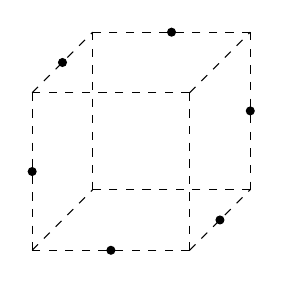
\begin{tikzpicture}
        % roots
        \draw[fill] (1,-1,0) circle (0.05);
        \draw[fill] (-1,1,0) circle (0.05);
        \draw[fill] (1,0,-1) circle (0.05);
        \draw[fill] (-1,0,1) circle (0.05);
        \draw[fill] (0,1,-1) circle (0.05);
        \draw[fill] (0,-1,1) circle (0.05);
        % cube
        \draw[dashed] (1,1,1) -- (1,1,-1);
        \draw[dashed] (1,-1,1) -- (1,-1,-1);
        \draw[dashed] (-1,1,1) -- (-1,1,-1);
        \draw[dashed] (-1,-1,1) -- (-1,-1,-1);
        \draw[dashed] (1,1,1) -- (1,-1,1);
        \draw[dashed] (1,1,-1) -- (1,-1,-1);
        \draw[dashed] (-1,1,1) -- (-1,-1,1);
        \draw[dashed] (-1,1,-1) -- (-1,-1,-1);
        \draw[dashed] (1,1,1) -- (-1,1,1);
        \draw[dashed] (1,-1,1) -- (-1,-1,1);
        \draw[dashed] (1,1,-1) -- (-1,1,-1);
        \draw[dashed] (1,-1,-1) -- (-1,-1,-1);
      \end{tikzpicture}
      \end{center}
      We see that in the subspace~$V$, which is the plane going through these six points, the roots form a regular hexagon:
      \begin{center}
      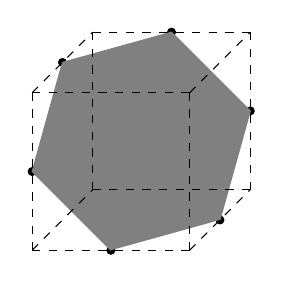
\begin{tikzpicture}
        % roots
        \draw[fill] (1,-1,0) circle (0.05);
        \draw[fill] (-1,1,0) circle (0.05);
        \draw[fill] (1,0,-1) circle (0.05);
        \draw[fill] (-1,0,1) circle (0.05);
        \draw[fill] (0,1,-1) circle (0.05);
        \draw[fill] (0,-1,1) circle (0.05);
        \draw[fill, gray] (1,-1,0) -- (1,0,-1) -- (0,1,-1) -- (-1,1,0) -- (-1,0,1) -- (0,-1,1);
        % cube
        \draw[dashed] (1,1,1) -- (1,1,-1);
        \draw[dashed] (1,-1,1) -- (1,-1,-1);
        \draw[dashed] (-1,1,1) -- (-1,1,-1);
        \draw[dashed] (-1,-1,1) -- (-1,-1,-1);
        \draw[dashed] (1,1,1) -- (1,-1,1);
        \draw[dashed] (1,1,-1) -- (1,-1,-1);
        \draw[dashed] (-1,1,1) -- (-1,-1,1);
        \draw[dashed] (-1,1,-1) -- (-1,-1,-1);
        \draw[dashed] (1,1,1) -- (-1,1,1);
        \draw[dashed] (1,-1,1) -- (-1,-1,1);
        \draw[dashed] (1,1,-1) -- (-1,1,-1);
        \draw[dashed] (1,-1,-1) -- (-1,-1,-1);
      \end{tikzpicture}
      \end{center}
      The root system therefore looks as follows:
      \begin{center}
      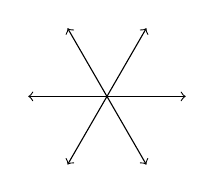
\begin{tikzpicture}
        \foreach \ang in {60, 120, ..., 360}{
          \draw[->] (0,0) -- (\ang:1);
        }
      \end{tikzpicture}
      \end{center}
      For~$n = 4$ the root system (which lives inside the {\fourdimensional} space~$\Real^4$) looks inside of its span~$V$ (which is {\threedimensional} as follows:
      \begin{center}
      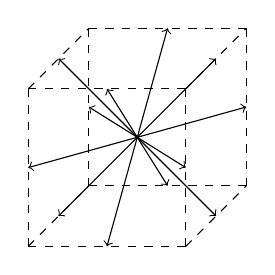
\begin{tikzpicture}
        % long roots
        \draw[->] (0,0,0) -- (1,1,0);
        \draw[->] (0,0,0) -- (1,-1,0);
        \draw[->] (0,0,0) -- (-1,1,0);
        \draw[->] (0,0,0) -- (-1,-1,0);
        \draw[->] (0,0,0) -- (1,0,1);
        \draw[->] (0,0,0) -- (1,0,-1);
        \draw[->] (0,0,0) -- (-1,0,1);
        \draw[->] (0,0,0) -- (-1,0,-1);
        \draw[->] (0,0,0) -- (0,1,1);
        \draw[->] (0,0,0) -- (0,1,-1);
        \draw[->] (0,0,0) -- (0,-1,1);
        \draw[->] (0,0,0) -- (0,-1,-1);
        % cube
        \draw[dashed] (1,1,1) -- (1,1,-1);
        \draw[dashed] (1,-1,1) -- (1,-1,-1);
        \draw[dashed] (-1,1,1) -- (-1,1,-1);
        \draw[dashed] (-1,-1,1) -- (-1,-1,-1);
        \draw[dashed] (1,1,1) -- (1,-1,1);
        \draw[dashed] (1,1,-1) -- (1,-1,-1);
        \draw[dashed] (-1,1,1) -- (-1,-1,1);
        \draw[dashed] (-1,1,-1) -- (-1,-1,-1);
        \draw[dashed] (1,1,1) -- (-1,1,1);
        \draw[dashed] (1,-1,1) -- (-1,-1,1);
        \draw[dashed] (1,1,-1) -- (-1,1,-1);
        \draw[dashed] (1,-1,-1) -- (-1,-1,-1);
      \end{tikzpicture}
      \end{center}
      The roots~$\pm e_i \pm e_j$ are the middle points of the edges of the ambient cube~$[-1,1]^3$.
      \begin{center}
      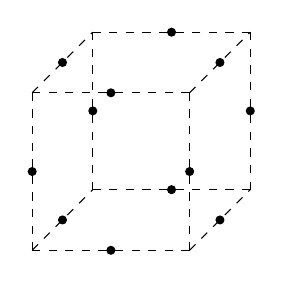
\begin{tikzpicture}
        % roots
        \draw[fill] (1,1,0) circle (0.05);
        \draw[fill] (1,-1,0) circle (0.05);
        \draw[fill] (-1,1,0) circle (0.05);
        \draw[fill] (-1,-1,0) circle (0.05);
        \draw[fill] (1,0,1) circle (0.05);
        \draw[fill] (1,0,-1) circle (0.05);
        \draw[fill] (-1,0,1) circle (0.05);
        \draw[fill] (-1,0,-1) circle (0.05);
        \draw[fill] (0,1,1) circle (0.05);
        \draw[fill] (0,1,-1) circle (0.05);
        \draw[fill] (0,-1,1) circle (0.05);
        \draw[fill] (0,-1,-1) circle (0.05);
        % cube
        \draw[dashed] (1,1,1) -- (1,1,-1);
        \draw[dashed] (1,-1,1) -- (1,-1,-1);
        \draw[dashed] (-1,1,1) -- (-1,1,-1);
        \draw[dashed] (-1,-1,1) -- (-1,-1,-1);
        \draw[dashed] (1,1,1) -- (1,-1,1);
        \draw[dashed] (1,1,-1) -- (1,-1,-1);
        \draw[dashed] (-1,1,1) -- (-1,-1,1);
        \draw[dashed] (-1,1,-1) -- (-1,-1,-1);
        \draw[dashed] (1,1,1) -- (-1,1,1);
        \draw[dashed] (1,-1,1) -- (-1,-1,1);
        \draw[dashed] (1,1,-1) -- (-1,1,-1);
        \draw[dashed] (1,-1,-1) -- (-1,-1,-1);
      \end{tikzpicture}
      \end{center}
      
    \item
      The set~$R = \{ \pm e_i \pm e_j \suchthat 1 \leq i \neq j \leq n \}$ is a reduced, crystallographic root system in~$\Real^n$ for~$n \geq 2$.
      
      The vector space~$\Real^n$ is spanned by~$R$ since~$e_i = (e_i - e_j)/2 + (e_i + e_j)/2$ for any~$j \neq i$.
      The reflection~$s_{e_i - e_j}$ swaps the two standard basis vectors~$e_i$ and~$e_j$, an operation under which~$R$ is closed.
      The reflection~$s_{e_i + e_j}$ again swaps the two standard basis vectors~$e_i$ and~$e_j$ but then also flips their signs.
      But this is again an operation under which~$R$ is closed.
      We thus find that~$R$ is indeed a root system.
      We see (directly) that it is reduced.
      We have for all~$1 \leq i \neq j \leq n$ and~$1 \leq k \neq l \leq n$ that
      \[
        2 \frac{(e_i \pm e_j, e_k \pm e_l)}{\norm{e_i \pm e_j}^2}
        =
        2 \frac{\delta_{ik} + \delta_{jl} \pm \delta_{il} \pm \delta_{jk}}{2}
        =
        \delta_{ik} + \delta_{jl} \pm \delta_{il} \pm \delta_{jk}
        \in
        \Integer \,,
      \]
      which shows that~$R$ is crystallographic.
      
      For small values of~$n$ these root systems look as follows:
      \begin{center}
        \begingroup
        \setlength{\tabcolsep}{24pt} %normal 6pt
        \begin{tabular}{cc}
          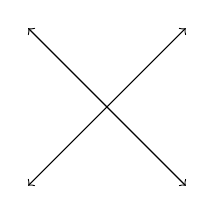
\begin{tikzpicture}
            % roots
            \draw[->] (0,0) -- (1,1);
            \draw[->] (0,0) -- (1,-1);
            \draw[->] (0,0) -- (-1,1);
            \draw[->] (0,0) -- (-1,-1);
          \end{tikzpicture}
          &
          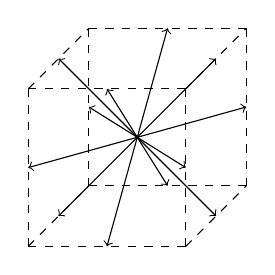
\begin{tikzpicture}
            % roots
            \draw[->] (0,0,0) -- (1,1,0);
            \draw[->] (0,0,0) -- (1,-1,0);
            \draw[->] (0,0,0) -- (-1,1,0);
            \draw[->] (0,0,0) -- (-1,-1,0);
            \draw[->] (0,0,0) -- (1,0,1);
            \draw[->] (0,0,0) -- (1,0,-1);
            \draw[->] (0,0,0) -- (-1,0,1);
            \draw[->] (0,0,0) -- (-1,0,-1);
            \draw[->] (0,0,0) -- (0,1,1);
            \draw[->] (0,0,0) -- (0,1,-1);
            \draw[->] (0,0,0) -- (0,-1,1);
            \draw[->] (0,0,0) -- (0,-1,-1);
            % cube
            \draw[dashed] (1,1,1) -- (1,1,-1);
            \draw[dashed] (1,-1,1) -- (1,-1,-1);
            \draw[dashed] (-1,1,1) -- (-1,1,-1);
            \draw[dashed] (-1,-1,1) -- (-1,-1,-1);
            \draw[dashed] (1,1,1) -- (1,-1,1);
            \draw[dashed] (1,1,-1) -- (1,-1,-1);
            \draw[dashed] (-1,1,1) -- (-1,-1,1);
            \draw[dashed] (-1,1,-1) -- (-1,-1,-1);
            \draw[dashed] (1,1,1) -- (-1,1,1);
            \draw[dashed] (1,-1,1) -- (-1,-1,1);
            \draw[dashed] (1,1,-1) -- (-1,1,-1);
            \draw[dashed] (1,-1,-1) -- (-1,-1,-1);
          \end{tikzpicture}
          \\
          $n = 2$
          &
          $n = 3$
        \end{tabular}
        \endgroup
      \end{center}
      In the case~$n = 3$ the roots~$\pm e_i \pm e_j$ are the middle points of the edges of the ambient cube~$[-1,1]^3$.
      \begin{center}
      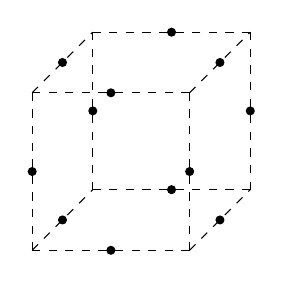
\begin{tikzpicture}
        % roots
        \draw[fill] (1,1,0) circle (0.05);
        \draw[fill] (1,-1,0) circle (0.05);
        \draw[fill] (-1,1,0) circle (0.05);
        \draw[fill] (-1,-1,0) circle (0.05);
        \draw[fill] (1,0,1) circle (0.05);
        \draw[fill] (1,0,-1) circle (0.05);
        \draw[fill] (-1,0,1) circle (0.05);
        \draw[fill] (-1,0,-1) circle (0.05);
        \draw[fill] (0,1,1) circle (0.05);
        \draw[fill] (0,1,-1) circle (0.05);
        \draw[fill] (0,-1,1) circle (0.05);
        \draw[fill] (0,-1,-1) circle (0.05);
        % cube
        \draw[dashed] (1,1,1) -- (1,1,-1);
        \draw[dashed] (1,-1,1) -- (1,-1,-1);
        \draw[dashed] (-1,1,1) -- (-1,1,-1);
        \draw[dashed] (-1,-1,1) -- (-1,-1,-1);
        \draw[dashed] (1,1,1) -- (1,-1,1);
        \draw[dashed] (1,1,-1) -- (1,-1,-1);
        \draw[dashed] (-1,1,1) -- (-1,-1,1);
        \draw[dashed] (-1,1,-1) -- (-1,-1,-1);
        \draw[dashed] (1,1,1) -- (-1,1,1);
        \draw[dashed] (1,-1,1) -- (-1,-1,1);
        \draw[dashed] (1,1,-1) -- (-1,1,-1);
        \draw[dashed] (1,-1,-1) -- (-1,-1,-1);
      \end{tikzpicture}
      \end{center}
    \item
      The set~$R = \{ \pm e_i \suchthat i = 1, \dotsc, n \} \cup \{ \pm e_i \pm e_j \suchthat 1 \leq i \neq j \leq n\}$ is a reduced, crystallographic root system in~$\Real^n$.
      
      The set~$R$ spans~$\Real^n$ it contains the standard basis.
      The reflection~$s_{e_i}$ swaps the sign of the standard basis vector~$e_i$, an operation under which~$R$ is invariant.
      The reflections~$s_{e_i - e_j}$ and~$s_{e_i + e_j}$ fix the standard basis vectors~$e_k$ with~$k \neq i,j$ and swap the standard basis vectors~$e_i$ and~$e_j$, while~$s_{e_i+e_j}$ then also flips the sign of~$e_i$ and~$e_j$.
      The set~$R$ is also invariant under these operations.
      This shows that~$R$ is indeed a root system and we see (directly) that it is reduced.
      
      To see that~$R$ is crystallographic we can reuse the calculations from the previous examples.
      It then remains to check that~$2 (\alpha, \beta)/\norm{\alpha}^2 \in \Integer$ for the cases~$\alpha = e_i$ and~$\beta = e_j \pm e_k$ with~$j \neq k$, and~$\beta = e_i \pm e_j$ and~$\alpha = e_k$ for~$i,j \neq k$.
      In the first case we have
      \[
        2 \frac{(e_i, e_j - e_k)}{\norm{e_i}^2}
        =
        2 \frac{\delta_{ij} - \delta_{ik}}{1}
        =
        2 \delta_{ij} - 2 \delta_{ik}
        \in
        \Integer
      \]
      and in the second case we have similarly
      \[
        2 \frac{(e_i - e_j, e_k)}{\norm{e_i - e_j}^2}
        =
        2 \frac{\delta_{ik} - \delta_{jk}}{2}
        =
        \delta_{ik} - \delta_{jk}
        \in
        \Integer \,.
      \]
      Thus~$R$ is crystallographic.
      
      For small values of~$n$ these root systems looks as follows:
      \begin{center}
      \begingroup
      \setlength{\tabcolsep}{18pt} %normal 6pt
      \begin{tabular}{ccc}
        \begin{tikzpicture}
          % center point
          \draw[fill] (0,0) circle (0.05);
          % roots
          \draw[->] (0,0) -- (1,0);
          \draw[->] (0,0) -- (-1,0);
          \draw[opacity=0] (0,0) -- (0,1);
          \draw[opacity=0] (0,0) -- (0,-1);
        \end{tikzpicture}
        &
        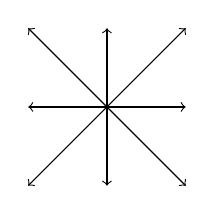
\begin{tikzpicture}
          % short roots
          \draw[->] (0,0) -- (1,0);
          \draw[->] (0,0) -- (-1,0);
          \draw[->] (0,0) -- (0,1);
          \draw[->] (0,0) -- (0,-1);
          % long rots
          \draw[->] (0,0) -- (1,1);
          \draw[->] (0,0) -- (1,-1);
          \draw[->] (0,0) -- (-1,1);
          \draw[->] (0,0) -- (-1,-1);
        \end{tikzpicture}
        &
        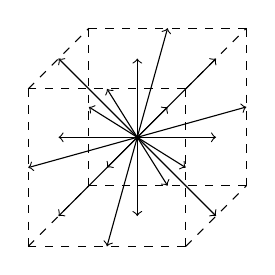
\begin{tikzpicture}
          % short roots
          \draw[->] (0,0,0) -- (1,0,0);
          \draw[->] (0,0,0) -- (-1,0,0);
          \draw[->] (0,0,0) -- (0,1,0);
          \draw[->] (0,0,0) -- (0,-1,0);
          \draw[->] (0,0,0) -- (0,0,1);
          \draw[->] (0,0,0) -- (0,0,-1);
          % long roots
          \draw[->] (0,0,0) -- (1,1,0);
          \draw[->] (0,0,0) -- (1,-1,0);
          \draw[->] (0,0,0) -- (-1,1,0);
          \draw[->] (0,0,0) -- (-1,-1,0);
          \draw[->] (0,0,0) -- (1,0,1);
          \draw[->] (0,0,0) -- (1,0,-1);
          \draw[->] (0,0,0) -- (-1,0,1);
          \draw[->] (0,0,0) -- (-1,0,-1);
          \draw[->] (0,0,0) -- (0,1,1);
          \draw[->] (0,0,0) -- (0,1,-1);
          \draw[->] (0,0,0) -- (0,-1,1);
          \draw[->] (0,0,0) -- (0,-1,-1);
          % cube
          \draw[dashed] (1,1,1) -- (1,1,-1);
          \draw[dashed] (1,-1,1) -- (1,-1,-1);
          \draw[dashed] (-1,1,1) -- (-1,1,-1);
          \draw[dashed] (-1,-1,1) -- (-1,-1,-1);
          \draw[dashed] (1,1,1) -- (1,-1,1);
          \draw[dashed] (1,1,-1) -- (1,-1,-1);
          \draw[dashed] (-1,1,1) -- (-1,-1,1);
          \draw[dashed] (-1,1,-1) -- (-1,-1,-1);
          \draw[dashed] (1,1,1) -- (-1,1,1);
          \draw[dashed] (1,-1,1) -- (-1,-1,1);
          \draw[dashed] (1,1,-1) -- (-1,1,-1);
          \draw[dashed] (1,-1,-1) -- (-1,-1,-1);
        \end{tikzpicture}
        \\
        $n = 1$
        &
        $n = 2$
        &
        $n = 3$
      \end{tabular}
      \endgroup
      \end{center}
      In the case~$n = 3$ the root system consists of the centers of the faces of the cube~$[-1,1]^3$ (these are the roots~$\pm e_i$) together with the middle points of the edges of the cube (these are the roots~$\pm e_i \pm e_j$).
      \begin{center}
        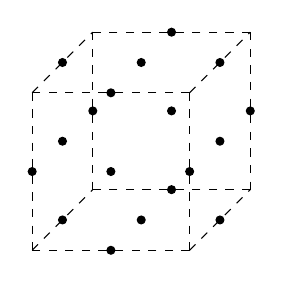
\begin{tikzpicture}
          % short roots
          \draw[fill] (1,0,0) circle (0.05);
          \draw[fill] (-1,0,0) circle (0.05);
          \draw[fill] (0,1,0) circle (0.05);
          \draw[fill] (0,-1,0) circle (0.05);
          \draw[fill] (0,0,1) circle (0.05);
          \draw[fill] (0,0,-1) circle (0.05);
          % long roots
          \draw[fill] (1,1,0) circle (0.05);
          \draw[fill] (1,-1,0) circle (0.05);
          \draw[fill] (-1,1,0) circle (0.05);
          \draw[fill] (-1,-1,0) circle (0.05);
          \draw[fill] (1,0,1) circle (0.05);
          \draw[fill] (1,0,-1) circle (0.05);
          \draw[fill] (-1,0,1) circle (0.05);
          \draw[fill] (-1,0,-1) circle (0.05);
          \draw[fill] (0,1,1) circle (0.05);
          \draw[fill] (0,1,-1) circle (0.05);
          \draw[fill] (0,-1,1) circle (0.05);
          \draw[fill] (0,-1,-1) circle (0.05);
          % cube
          \draw[dashed] (1,1,1) -- (1,1,-1);
          \draw[dashed] (1,-1,1) -- (1,-1,-1);
          \draw[dashed] (-1,1,1) -- (-1,1,-1);
          \draw[dashed] (-1,-1,1) -- (-1,-1,-1);
          \draw[dashed] (1,1,1) -- (1,-1,1);
          \draw[dashed] (1,1,-1) -- (1,-1,-1);
          \draw[dashed] (-1,1,1) -- (-1,-1,1);
          \draw[dashed] (-1,1,-1) -- (-1,-1,-1);
          \draw[dashed] (1,1,1) -- (-1,1,1);
          \draw[dashed] (1,-1,1) -- (-1,-1,1);
          \draw[dashed] (1,1,-1) -- (-1,1,-1);
          \draw[dashed] (1,-1,-1) -- (-1,-1,-1);
        \end{tikzpicture}
        \end{center}
    \item
      The set~$R = \{ \pm 2 e_i \suchthat i = 1, \dotsc, n \} \cup \{ \pm e_i \pm e_j \suchthat 1 \leq i \neq j \leq n\}$ is a reduced, crystallographic root system in~$\Real^n$.
      That~$R$ is a reduced root system can be seen in the same way as in the previous example.
      To see that~$R$ is crystallographic we calculate as in the previous case that
      \begin{gather*}
        2 \frac{(2e_i, e_j - e_k)}{\norm{2 e_i}^2}
        =
        2 \frac{2\delta_{ij} - 2\delta_{ik}}{4}
        =
        \delta_{ij} - 2 \delta_{ik}
        \in
        \Integer
      \shortintertext{and}
        2 \frac{(e_i - e_j, 2 e_k)}{\norm{e_i - e_j}^2}
        =
        2 \frac{2 \delta_{ik} - 2 \delta_{jk}}{2}
        =
        4 \delta_{ik} - \delta_{jk}
        \in
        \Integer \,.
      \end{gather*}
      
      For small values of~$n$ these root systems looks as follows:
      \begin{center}
      \begingroup
      \setlength{\tabcolsep}{12pt} %normal 6pt
      \begin{tabular}{ccc}
        \begin{tikzpicture}[scale=0.7]
          % center point
          \draw[fill] (0,0) circle (0.05);
          % roots
          \draw[->] (0,0) -- (2,0);
          \draw[->] (0,0) -- (-2,0);
          \draw[opacity=0] (0,0) -- (0,2);
          \draw[opacity=0] (0,0) -- (0,-2);
        \end{tikzpicture}
        &
        \begin{tikzpicture}[scale=0.7]
          % short roots
          \draw[->] (0,0) -- (2,0);
          \draw[->] (0,0) -- (-2,0);
          \draw[->] (0,0) -- (0,2);
          \draw[->] (0,0) -- (0,-2);
          % long rots
          \draw[->] (0,0) -- (1,1);
          \draw[->] (0,0) -- (1,-1);
          \draw[->] (0,0) -- (-1,1);
          \draw[->] (0,0) -- (-1,-1);
        \end{tikzpicture}
        &
        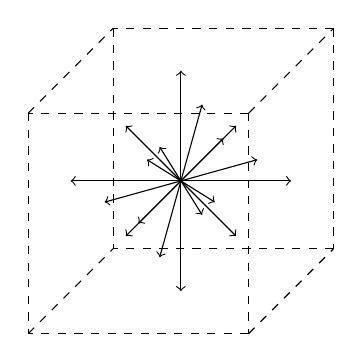
\begin{tikzpicture}[scale=0.7]
          % short roots
          \draw[->] (0,0,0) -- (2,0,0);
          \draw[->] (0,0,0) -- (-2,0,0);
          \draw[->] (0,0,0) -- (0,2,0);
          \draw[->] (0,0,0) -- (0,-2,0);
          \draw[->] (0,0,0) -- (0,0,2);
          \draw[->] (0,0,0) -- (0,0,-2);
          % long roots
          \draw[->] (0,0,0) -- (1,1,0);
          \draw[->] (0,0,0) -- (1,-1,0);
          \draw[->] (0,0,0) -- (-1,1,0);
          \draw[->] (0,0,0) -- (-1,-1,0);
          \draw[->] (0,0,0) -- (1,0,1);
          \draw[->] (0,0,0) -- (1,0,-1);
          \draw[->] (0,0,0) -- (-1,0,1);
          \draw[->] (0,0,0) -- (-1,0,-1);
          \draw[->] (0,0,0) -- (0,1,1);
          \draw[->] (0,0,0) -- (0,1,-1);
          \draw[->] (0,0,0) -- (0,-1,1);
          \draw[->] (0,0,0) -- (0,-1,-1);
          % cube
          \draw[dashed] (2,2,2) -- (2,2,-2);
          \draw[dashed] (2,-2,2) -- (2,-2,-2);
          \draw[dashed] (-2,2,2) -- (-2,2,-2);
          \draw[dashed] (-2,-2,2) -- (-2,-2,-2);
          \draw[dashed] (2,2,2) -- (2,-2,2);
          \draw[dashed] (2,2,-2) -- (2,-2,-2);
          \draw[dashed] (-2,2,2) -- (-2,-2,2);
          \draw[dashed] (-2,2,-2) -- (-2,-2,-2);
          \draw[dashed] (2,2,2) -- (-2,2,2);
          \draw[dashed] (2,-2,2) -- (-2,-2,2);
          \draw[dashed] (2,2,-2) -- (-2,2,-2);
          \draw[dashed] (2,-2,-2) -- (-2,-2,-2);
        \end{tikzpicture}
        \\
        $n = 1$
        &
        $n = 2$
        &
        $n = 3$
      \end{tabular}
      \endgroup
      \end{center}
    \item
      Let~$n \geq 1$ and let~$R$ be the subset of~$\Real^2$ given by
      \[
        R
        =
        \left\{
          \left(
            \cos\left( k \cdot \frac{\pi}{n} \right),
            \sin\left( k \cdot \frac{\pi}{n} \right) 
          \right)
        \suchthat*
          k = 0, \dotsc, 2n-1
        \right\}
      \]
      This means that~$R$ consists of the vertices of a regular~{\gon{$2n$}}, and for small~$n$ we can visualize~$R$ as follows:
      \[
        \begingroup
        \renewcommand{\arraystretch}{1.5}
        \begin{array}{cccc}
          \vcenter{
          \hbox{
          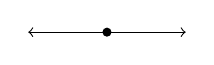
\begin{tikzpicture}
            \draw[->] (0,0) -- (1,0);
            \draw[->] (0,0) -- (-1,0);
            \draw[fill] (0,0) circle (0.05);
          \end{tikzpicture}
          }
          }
          &
          \vcenter{
          \hbox{
          \begin{tikzpicture}
            \foreach \ang in {90, 180, 270, 360}{
              \draw[->] (0,0) -- (\ang:1);
%              \draw[fill] (\ang:1) circle (0.05);
%              \draw (\ang:1) -- (\ang+90:1);
            }
          \end{tikzpicture}
          }
          }
          &
          \vcenter{
          \hbox{
          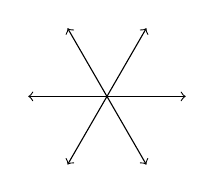
\begin{tikzpicture}
            \foreach \ang in {60, 120, ..., 360}{
              \draw[->] (0,0) -- (\ang:1);
%              \draw (\ang:1) -- (\ang+60:1);
            }
          \end{tikzpicture}
          }
          }
          &
          \vcenter{
          \hbox{
          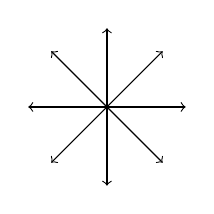
\begin{tikzpicture}
            \foreach \ang in {45, 90, ..., 360}{
              \draw[->] (0,0) -- (\ang:1);
%              \draw (\ang:1) -- (\ang+45:1);
            }
          \end{tikzpicture}
          }
          }
          \\
          n = 1
          &
          n = 2
          &
          n = 3
          &
          n = 4
        \end{array}
        \endgroup
      \]
      We see (directly) that~$R$ is always a reduced root system.
      For~$n = 1, 2, 3$ we have already encountered these root systems above, and have seen that they are crystallographic.
      But for~$n \geq 4$ this is not the case:
      Let~$\alpha, \beta \in R$ and let~$\theta$ be the unoriented angle between~$\alpha$ and~$\beta$, i.e.~$\beta \in [0,\pi]$.Then
      \[
        2 \frac{(\alpha, \beta)}{\norm{\alpha}^2}
        =
        2 (\alpha, \beta)
        =
        2 \cos(\theta) \norm{\alpha} \norm{\beta}
        =
        2 \cos(\theta)
      \]
      because~$\norm{\alpha} = \norm{\beta}$.
      For~$R$ to be crystallographic we need~$2 \cos(\theta) \in \Integer$ and thus
      \begin{gather*}
        \cos(\theta)
        \in
        \left\{
          0,
          \pm \frac{1}{2},
          \pm 1
        \right\} \,,
      \shortintertext{which means that}
        \theta
        \in
        \left\{
          \frac{\pi}{2},
          \frac{\pi}{3},
          \frac{2\pi}{3},
          0,
          \pi
        \right\} \,.
      \end{gather*}
      But for~$n \geq 4$ there exist two roots in~$R$ for which the angle between them is smaller or equal to~$\pi/4$.
      (One can take two neighbouring vertices of the regular~{\gon{$n$}} to get the angle~$\pi/n$.)
    \item
      Let~$R$ be the subset of~$\Real^2$ given by
      \begin{align*}
        R
        ={}&
        \left\{
          \left(
            \cos\left( k \cdot \frac{\pi}{3} \right),
            \sin\left( k \cdot \frac{\pi}{3} \right) 
          \right)
        \suchthat*
          k = 0, \dotsc, 5
        \right\}
        \\
        {}&
        \cup
        \left\{
          \sqrt{3}
          \left(
            \cos\left( k \cdot \frac{\pi}{3} + \frac{\pi}{6} \right),
            \sin\left( k \cdot \frac{\pi}{3} + \frac{\pi}{6} \right) 
          \right)
        \suchthat*
          k = 0, \dotsc, 5
        \right\}
      \end{align*}
      The following picture is probably more instructive:
      \begin{center}
      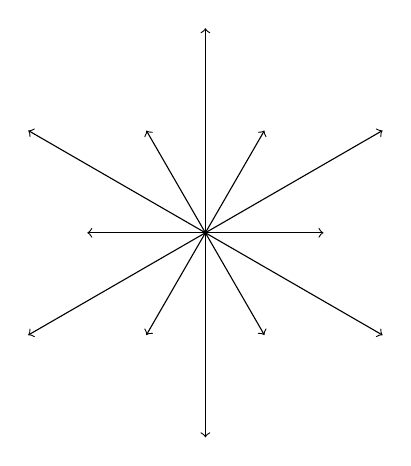
\begin{tikzpicture}[scale = 1.5]
        \foreach \ang in {60, 120, ..., 360}{
          \draw[->] (0,0) -- (\ang:1);
          \draw[->] (0,0) -- (\ang + 30 : 1.732);
        }
      \end{tikzpicture}
      \end{center}
      We see that~$\Real^2$ is spanned by~$R$ and that for every~$\alpha \in R$ the set~$R$ is invariant under the reflection~$s_\alpha$.
      Hence~$R$ is a root system.
      We also see that (directly)~$R$ is reduced.
      By looking long enough at the above picture we also see that~$s_\alpha(\beta) \in \beta + \Integer \alpha$ for all~$\alpha, \beta \in R$, i.e.\ that~$R$ is crystallographic.
  \end{enumerate}
\end{examples}


\begin{examples}
  Some of the examples from \cref{root systems in Rn} can be generalized to general~{\vectorspaces{$\kf$}}:
  \begin{enumerate}
    \item
      We denote for every~$n \geq 1$ by~$\rootA_n$ the root system of rank~$n$ in the vector space
      \begin{align*}
        V
        =
        \{
          (x_1, \dotsc, x_{n+1})
          \in
          \kf^{n+1}
        \suchthat
          x_1 + \dotsb + x_n = 0
        \}
      \shortintertext{that is given by}
        \rootA_n
        =
        \{
          e_i - e_j
        \suchthat
          1 \leq i \neq j \leq n+1
        \} \,.
      \end{align*}
      For all~$1 \leq i \neq j \leq n$ the reflection~$s_{e_i-e_j} \colon V \to V$ is the restriction of the reflection~$\kf^{n+1} \to \kf^{n+1}$ that swaps the standard basis vectors~$e_i$ and~$e_j$ and fixes pointwise all other standard basis vectors.
    \item
      We denote for every~$n \geq 2$ by~$\rootB_n$ the root system of rank~$n$ in the vector space~$\kf^n$ that is given by
      \[
        \rootB_n
        \defined
        \{
          \pm e_i
        \suchthat
          i = 1, \dotsc, n
        \}
        \cup
        \{
          \pm e_i \pm e_j
        \suchthat
          1 \leq i \neq j \leq n
        \} \,.
      \]
      The reflections~$s_{e_i}$ are given by flipping the sign of the standard basis vector~$e_i$, the reflections~$s_{e_i - e_j}$ are given as above by swapping the standard basis vectors~$e_i$ and~$e_j$, and the reflections~$s_{e_i + e_j}$ are given by both swapping the standard basis vectors~$e_i$ and~$e_j$ while also flipping their signs.
    \item
      We denote for every~$n \geq 2$ by~$\rootC_n$ the root system of rank~$n$ in the vector space~$\kf^n$ that is given by
      \[
        \rootC_n
        \defined
        \{
          \pm 2 e_i
        \suchthat
          i = 1, \dotsc, n
        \}
        \cup
        \{
          \pm e_i \pm e_j
        \suchthat
          1 \leq i \neq j \leq n
        \} \,.
      \]
      The reflections associated to~$\rootC_n$ are the same as for~$\rootB_n$, with~$s_{2e_i} = s_{e_i}$.
    \item
      We denote for every~$n \geq 2$ by~$\rootD_n$ the root system of rank~$n$ in the vector space~$\kf^n$ that is given by
      \[
        \rootD_n
        \defined
        \{
          \pm e_i \pm e_j
        \suchthat
          1 \leq i \neq j \leq n
        \} \,.
      \]
      The reflections~$s_{e_i - e_j}$ are as described above.
  \end{enumerate}
\end{examples}


\begin{remark}
  \label{standard root systems have isometric reflections}
  Let~$\inner{-,-}$ be the standard symmetric bilinear form on~$\kf^n$, i.e.~$\inner{x,y} = \sum_{i=1}^n x_i y_i$.
  Then for the root systems~$\rootB_n$,~$\rootC_n$ and~$\rootD_n$ the reflections~$s_\alpha$, where~$\alpha$ is some root, are isometries for~$\inner{-,-}$:
  The standard basis~$e_1, \dotsc, e_n$ of~$\kf^n$ is an orthonormal basis of~$\kf^n$ whence~$s_\alpha$ is an isometry if and only if its representing matrix with respect to this basis is orthogonal.
  This can be seen in (at least) two ways:
  \begin{itemize}
    \item
      Using the above explicit descriptions of these reflections we can write down these matrices and check the assertion by hand.
    \item
      We see from the above explicit description of these reflections that their representing matrices with respect to the standard basis have integer entries (namely~$0$ and~$\pm 1$).
      The claim does therefore not depend on the choice of ground field~$\kf$.
      But we have seen in \cref{root systems in Rn} that the assertion holds for~$\kf = \Real$ (where the standard symmetric form becomes the standard inner product).
      Hence it holds for general~$\kf$.
  \end{itemize}
  
  The reflections~$s_\alpha$ for~$\alpha \in \rootA_n$ are restrictions of reflections~$s'_\alpha$ of~$\kf^n$, which can be shown to be isometries with respect to~$\inner{-,-}$ in the same way as above.
  It follows that~$s_\alpha$ is an isometry with respect to the restriction of~$\inner{-,-}$ to the subspace in which~$\rootA_n$ is a root system.
\end{remark}






\subsection{The Weyl Group}


\begin{definition}
  The \defemph{Weyl~group}\index{Weyl group} of a root system~$R$ in a~{\vectorspace{$\kf$}}~$V$ is the subgroup~$\Weyl(R)$ of~$\GL(V)$ generated by all reflections~$s_\alpha$ with~$\alpha \in R$.
\end{definition}


\begin{remark}
  Let~$R$ be a root system in a~{\vectorspace{$\kf$}}~$V$.
  Every group element~$w \in \Weyl(R)$ leaves the set~$R$ invariant because this holds for the generators~$s_\alpha$ with~$\alpha \in R$.
  The Weyl group~$\Weyl(R)$ therefore acts on the root system~$R$ by restriction of the action on~$V$.
  Every element~$w \in W$ is furthermore uniquely determined by the restriction~$\restrict{w}{R}$ because the set~$R$ spans the vector space~$V$.
  The action of~$\Weyl(R)$ on~$R$ is therefore faithful whence we can identify the Weyl~group~$\Weyl(R)$ with a subgroup of the symmetric group on~$R$.
  We see in particular that the Weyl~group~$\Weyl(R)$ is finite because~$R$ is finite.
\end{remark}


\begin{examples}
  Let us calculate the Weyl~groups of some root systems.
  \begin{enumerate}
    \item
      The only root system in the zero vector space~$0$ is the empty root system~$R = \emptyset$.
      Its Weyl~group is generated by the empty set and is thus the trivial group.
    \item
      The only reflection in a {\onedimensional} vector space~$V$ is the inversion map~$s \colon V \to V$ given by~$x \mapsto -x$.
      Any root system~$R$ in~$V$ is nonempty since it spans~$V$. 
      The Weyl~group~$\Weyl(R)$ does therefore admit nontrivial generators, all of which are necessarily the reflection~$s$.
      This shows that~$\Weyl(R) = \gen{s} \cong \Integer/2$.
    \item
      For our first interesting example we consider the root system~$\rootA_n = \{ e_i - e_j \suchthat 1 \leq i \neq j \leq n+1 \}$ in the~{\vectorspace{$\kf$}}~$V = \{ (x_1, \dotsc, x_{n+1}) \in \kf^{n+1} \suchthat x_1 + \dotsb + x_{n+1} = 0 \}$.
      We will show that its Weyl~group is (isomorphic to) the symmetric group~$\symm_{n+1}$.
      We will construct an isomorphism under which the reflection~$s_{e_i - e_j}$ corresponds to the transposition~$(i,j)$.
      
      The reflection~$s_{e_i - e_j} \colon V \to V$ is the restriction of the reflection~$s'_{e_i - e_j} \colon \kf^{n+1} \to \kf^{n+1}$ that swaps the standard basis vectors~$e_i$ and~$e_j$ and fixes all the other standard basis vectors.
      The subgroup~$W'$ of~$\GL(\kf^{n+1})$ that is generated by the reflections~$s'_\alpha$ with~$\alpha \in \rootA_n$ is the symmetric group~$\symm_{n+1}$, so that the reflecton~$s'_{e_i - e_j}$ corresponds to the transposition~$(i,j)$.
      
      We have a surjective group homomorphism~$r \colon W' \to \Weyl(\rootA_n)$ given by~$w \mapsto \restrict{w}{V}$ because the generator~$s'_\alpha$ of~$W$ restrict to the generator~$s_\alpha$ of~$\Weyl(\rootA_n)$.
      We claim that~$r$ is injective, and thus a group isomorphism.
      This then establishes an isomorphism~$\Weyl(\rootA_n) \cong W' \cong \symm_{n+1}$ under which the reflection~$s_{e_i - e_j}$ corresponds to the transposition~$(i,j)$.
      
      That the group homomorphism~$r \colon W' \to \Weyl(\rootA_n)$ is injective means precisely that~$V$ is faithful as an~{\representation{$\symm_{n+1}$}}, where~$\symm_{n+1}$ acts by permutation of the standard basis vectors.
      To show this faithfulness we consider the decomposition~$\kf^{n+1} = V \oplus L$ with~$L = \gen{(1, \dotsc, 1)}_{\kf}$.
      The permutation action of~$\symm_{n+1}$ on~$\kf^{n+1}$ is faithful and trivial on the subrepresentation~$L$.
      Hence the action of~$\symm_{n+1}$ on the direct summand~$V$ needs to be faithful.
    \item
      Let us now consider the root system~$\rootB_n = \{ \pm e_i \suchthat i = 1, \dotsc, n \} \cup \{ \pm e_i \pm e_j \suchthat 1 \leq i \neq j \leq n \}$ in the vector space~$V = \kf^n$.
      
      The reflection~$s_{e_i}$ flips the sign of the standard basis vector~$e_i$ and fixes all other standard basis vectors.
      The reflection~$s_{e_i - e_j}$ swaps the two standard basis vectors~$e_i$ and~$e_j$ and fixes all other standard basis vectors.
      The reflection~$s_{e_i + e_j}$ swaps the two standard basis vectors~$e_i$ and~$e_j$ and also swappes their signs, and fixes all other standard basis vectors.
      
      We see from these explicit descriptions of the reflections~$s_\alpha$ with~$\alpha \in R$ that these reflections are with respect to the standard basis of~$\kf^n$ given by signed permutation matrices.%
      \footnote{A \defemph{signed permutation matrix}\index{signed permutation matrix} is a matrix that admits in every column and every row precisely one nonzero entry, that is allowed to take on the values~$1$ and~$-1$.
      A signed permutation matrix does therefore have the same form as a permutation matrix, but the occuring nonzero entries need not be~$1$ but are also allowed to be~$-1$.}
      Let us for now identify the group~$\GL(\kf^n)$ with the matrix group~$\GL_n(\kf)$ by identifying each endomorphism of~$\kf^n$ with its representing matrix with respect to the standard basis~$e_1, \dotsc, e_n$.
      The elements of the Weyl~group~$\Weyl(\rootB_n)$ are thus identified with signed permutation matrices.
      
      The reflections~$s_{e_i - e_j}$ with~$1 \leq i \neq j \leq n$ generate the group of permutation matrices (as seen in the previous example).
      The reflections~$s_{e_i}$ with~$i = 1, \dotsc, n$ generate the group of diagonal matrices with diagonal entries~$\pm 1$.
      Every signed permutation matrix is a product of two such matrices.
      Thus we find that~$\Weyl(\rootB_n)$ is the full group fo signed permutation matrices.
      
      The group~$D$ is normalized by~$P$, and every element of~$\Weyl(\rootB_n)$ can be uniquely written as a product~$dp$ with~$d \in D$ and~$p \in P$.
      This means that~$\Weyl(\rootB_n)$ is the semidirect product of its subgroups~$D$ and~$P$, which~$D$ being the normal factor, i.e.~$\Weyl(\rootB_n) = D \rtimes P$.
      The group of~$P$ of permutation matrices is isomorphic to the symmetric group~$\symm_n$, whereas the group~$D$ of diagonal matrices with diagonal entries~$\pm 1$ is isomorphic to the group~$(\Integer/2)^n$.
      We find altogether that
      \[
        \Weyl(\rootB_n)
        \cong
        \{ \text{signed permutation matrices} \}
        =
        D \rtimes P
        \cong
        (\Integer/2)^n \rtimes \symm_n \,.
      \]
    \item
      For the root system~$\rootC_n = \{ \pm 2 e_i \suchthat i = 1, \dotsc, n \} \cup \{ \pm e_i \pm e_j \suchthat 1 \leq i \neq j \leq n \}$ we find that~$s_{2e_i} = s_{e_i}$ where~$s_{e_i}$ are the above reflections for the root system~$\rootB_n$.
      The Weyl~groups~$\Weyl(\rootB_n)$ and~$\Weyl(\rootC_n)$ are therefore two subgroups of~$\GL(\kf^n)$ that admit the same generating set.
      We thus find that~$\Weyl(\rootC_n) = \Weyl(\rootB_n)$.
    \item
      Let us now consider the root system~$\rootD_n = \{ \pm e_i \pm e_j \suchthat 1 \leq i \neq j \leq n \}$ in~$V = \kf^n$.
      We see as before that the reflections~$s_{\pm e_i \pm e_j}$ are with respect to the standard basis~$e_1, \dotsc, e_n$ of~$\kf^n$ represented by certain signed permutation matrices.
      By considering the reflections~$s_{e_i - e_j}$ we see again that~$\Weyl(R)$ contains the group~$P$ of permutation matrices.
      The composition~$s_{e_i - e_j} \circ s_{e_i + e_j}$ flips the sign of the two standard basis vectors~$e_i$ and~$e_j$ and fixes all other standard basis vectors.
      It follows that~$\Weyl(R)$ contains the group~$D'$ of diagonal matrices whose diagonal entries are~$\pm 1$ and for which the diagonal entry~$-1$ appear an even number of times.
      The subgroup~$D'$ is normalized by the subgroup~$P$ whence~$D'P$ is again subgroup of~$\Weyl(R)$.
      The generators~$s_{e_i - e_j}$ are contained in~$P$ and thus in~$D' P$.
      The generators~$s_{e_i + e_j} = s_{e_i - e_j} \circ (s_{e_i - e_j} \circ s_{e_i + e_j})$ are contained in~$D' P$ because~$s_{e_i - e_j} \circ s_{e_i + e_j}$ is contained in~$D'$ and~$s_{e_i - e_j}$ is contained in~$P$.
      Thus~$\Weyl(R) = D' P$.
      
      We have altogether found that~$\Weyl(R) = D' P$ where~$D'$ is normalized by~$P$, and we see that~$D'$ and~$P$ intersect only trivially.
      This shows that~$\Weyl(R) = D' \rtimes P$ is the internal semidirect product of~$D'$ and~$P$.
      The group~$D'$ is isomorphic to~$(\Integer/2)^{n-1}$ and the group~$P$ is isomorphic to the symmetric group~$S_n$.
      Whence
      \[
        \Weyl(R)
        \cong
        D' \rtimes P
        \cong
        (\Integer/2)^{n-1} \rtimes S_n \,.
      \]
      The product~$D' P$ consists precisely of the signed permutation matrices which admit an even number of~$-1$’s.
%   TODO: Weyl group of I_n is D_n.
  \end{enumerate}
\end{examples}


\begin{lemma}
  \label{reflection of conjugated root}
  Let~$R$ be a root system in a~{\vectorspace{$\kf$}}~$V$.
  For every root~$\alpha \in R$ and every group element~$w \in \Weyl(R)$ the reflection associated to the root~$w(\alpha)$ is given by
  \[
    s_{w(\alpha)}
    =
    w \circ s_\alpha \circ w^{-1} \,.
  \]
\end{lemma}


\begin{proof}
  The composition~$w \circ s_\alpha \circ w^{-1}$ is similar to the reflection~$s_\alpha$ and therefore again a reflection (since reflections are characterized by their eigenvalues).
  The composition~$w \circ s_\alpha \circ w^{-1}$ maps~$R$ into itself (since all three factors do this) and it flip the vector~$w(\alpha)$.
  This shows that the composition~$w \circ s_\alpha \circ w^{-1}$ satisfies the defining properties of the reflection~$s_{w(\alpha)}$.
\end{proof}


\begin{lemma}
  \label{weyl groups fixes no line}
  Let~$R$ be a root system in a~{\vectorspace{$\kf$}}~$V$.
  The only vector~$v \in V$ that is fixed by every group element~$w \in \Weyl(R)$ is the zero vector~$v = 0$.
  Thus no line in~$V$ is fixed pointwise by the Weyl~group.
\end{lemma}


\begin{proof}
  Suppose that a vector~$v \in V$ is fixed by every element of the Weyl~group~$\Weyl(R)$.
  The line~$L \defined \kf v$ is then a~{\subrepresentation{$\Weyl(R)$}} of~$V$ (on which~$\Weyl(R)$ acts trivially).
  There exists by Maschke’s~theorem a complementary subrepresentation to~$L$, i.e.\ a subrepresentation~$U$ of~$V$ with~$V = L \oplus C$.
  
  Let~$\alpha \in R$ be a root.
  The reflection~$s_\alpha$ acts non-trivially on~$V$ and thus acts non-trivially on one of the two subrepresentations~$L$ or~$C$.
  We thus find that~$s_\alpha$ acts non-trivially on~$C$.
  It follows from \cref{subspaces invariant under reflection} that~$\alpha$ is contained in~$C$.
  This shows that the subrepresentation~$C$ contains all roots.
  It follows that~$C = V$ since~$R$ is a generating set for the vector space~$V$.
  Therefore~$L = 0$ and thus~$v = 0$.
\end{proof}





\subsection{Irreducible Decomposition}

% TODOO: Examples

\begin{lemma}
  \label{induced root system of subspace}
  Let~$R$ be a root system in a {\vectorspace{$\kf$}}~$V$ and let~$U$ be a linear subspace of~$V$.
  Then the intersection~$R' \defined R \cap U$ is a root system in its span~$U' \defined \gen{R'}$.
  If~$R$ is reduced or crystallographic then the same holds for~$R'$.
%   The inclusion~$(R', U') \to (R, U)$ is a homomorphism of root systems.
\end{lemma}


\begin{proof}
  It follows from \cref{subspaces invariant under reflection} that~$U'$ is~{\invariant{$s_\alpha$}} for every~$\alpha \in R'$ since~$U'$ contains the flipped vector~$\alpha$.
  We can therefore consider for every~$\alpha \in R'$ the restriction~$s'_\alpha \defined \restrict{s_\alpha}{U'}$.
  This restriction is again a reflection:
  We have~$s'_\alpha(\alpha) = -\alpha$ and~$s'_\alpha(v) = s_\alpha(v) \in v + \kf \alpha$ for every vector~$v \in V$.
  We can therefore apply characterization~\ref{maps all vectors into lines} of~\cref{characterizations of reflections} to see the claim.
  
  The restriction~$s'_\alpha$ satisfies~$s'_\alpha(\beta) = s_\alpha(\beta) \in R$ for every root~$\beta \in R'$, and by \cref{reflected vector is a linear combination} also~$s'_\alpha(\beta) = s_\alpha(\beta) \in U$.
  Thus~$s_\alpha(\beta) \in R \cap U = R'$.
  We have shown that~$R'$ is a root system in~$U'$ with associated reflections~$s'_\alpha$ for~$\alpha \in R'$.
  
  We have for every~$\alpha \in R'$ that~$\kf \alpha \cap R' = \kf \alpha \cap U \cap R = \kf \alpha \cap R$, so if~$R$ is reduced then~$R'$ is also reduced.
  If the crystallographic condition~$s_\alpha(\beta) \in \beta + \Integer \alpha$ is satisfied for~$R$ then it is in particular satisfied in~$R'$.
%   The inclusion~$(R', U') \to (R, V)$ is a homomorphism of root systems since for~$\alpha \in R'$ the reflection~$s'_\alpha$ is the restriction of the reflection~$s_\alpha$.
\end{proof}


\begin{proposition}
  \label{decomposition of root systems}
  Let~$R$ be a root system in a~{\vectorspace{$\kf$}}~$V$.
  Let~$R_1, \dotsc, R_n \subseteq R$ be subsets with~$R = R_1 \cup \dotsb \cup R_n$.
  For every~$i = 1, \dotsc, n$ let~$V_i$ be the span of~$R_i$.
  Then the following two conditions are equivalent:
  \begin{equivalenceslist}
    \item
      \label{decomposition as vector spaces}
      $V = V_1 \oplus \dotsb \oplus V_n$.
    \item
      \label{leaving others invariant}
      $s_\alpha(\beta) = \beta$ for all~$\alpha \in R_i$ and all~$\beta \in R_j$ with~$i \neq j$.
  \end{equivalenceslist}
  If these conditions are satisfied then each~$R_i$ is a root system in its span~$V_i$, and~$R$ is the disjoint union of~$R_1, \dotsc, R_n$.
  For every root~$\alpha \in R_i$ the reflection~$s_\alpha$ fixes pointwise the direct summands~$V_j$ with~$j \neq i$.
\end{proposition}


\begin{proof}
  \leavevmode
  \begin{implicationlist}
    \item[\ref*{decomposition as vector spaces}~$\implies$~\ref*{leaving others invariant}]
      We know from \cref{reflected vector is a linear combination} that~$s_\alpha(\beta) \in \beta + \kf \alpha$.
      But the vectors~$\alpha$ and~$\beta$ are contained in distinct direct summand of the decomposition~$V = V_1 \oplus \dotsb \oplus V_n$.
      Hence the only element of the line~$\beta + \kf \alpha$ that is again contained in some direct summand is~$\beta$ itself.
      But~$s_\alpha(\beta)$ is again a root and therefore contained in some set~$R_k$, and thus also in the corresponding direct summand~$V_k$.
      Thus we must have~$s_\alpha(\beta) = \beta$.
    \item[\ref*{leaving others invariant}~$\implies$~\ref*{decomposition as vector spaces}]
      We first observe that for every root~$\alpha \in R_i$ and index~$j \neq i$ the reflection~$s_{\alpha_i}$ fixes pointwise all roots~$\beta \in R_j$ and thus acts trivially on the linear subspace~$\gen{R_j}_{\kf} = V_j$.

      To show that~~$V = V_1 \oplus \dotsb \oplus V_n$ we note that
      \[
        V_1 + \dotsb + V_n
        =
        \gen{R_1}_{\kf} + \dotsb + \gen{R_n}_{\kf}
        =
        \gen{R_1 \cup \dotsb \cup R_n}_{\kf}
        =
        \gen{R}_{\kf}
        =
        V \,.
      \]
      To show the directness of this sum let
      \[
        v_i = \sum_{j \neq i} v_j 
      \]
      for some vector~$v_i \in V_i$ and some summands~$v_j \in V_j$ for~$j \neq i$.
      It follows from the above observation that the reflections~$s_\alpha$ with~$\alpha \in R_i$ fix the summands~$v_j$ for all~$j \neq i$.
      These reflections do therefore fix the vector~$v_i$.
      We also find from the above obsveration that the reflections~$s_\alpha$ with~$\alpha \in R_j$ for~$j \neq i$ fix the vector~$v_i$.
      This shows that the vector~$v_i$ is fixed by every reflection~$\alpha \in R$.
      It follows from \cref{induced root system of subspace} that~$v_i = 0$.
  \end{implicationlist}
  
  We have seen above the assertion that any reflection~$s_\alpha$ with~$\alpha \in R_i$ fixes pointwise the direct summands~$V_j$ with~$j \neq i$.
  The disjointness of the decomposition~$R = R_1 \cup \dotsb \cup R_n$ follows from the directness of the sum~$V = V_1 \oplus \dotsb \oplus V_n$ since the only common element of~$V_i$ and~$V_j$ with~$i \neq j$ is the zero vector, which is not contained in~$R$.
  That~$R_i$ is a root system in~$V_i$ follows from \cref{induced root system of subspace} because~$R \cap V_i = R_i$ with~$R_i$ spanning~$V_i$.
\end{proof}


\begin{definition}
  Let~$R$ be a root system in a~{\vectorspace{$\kf$}}~$V$.
  \begin{enumerate}
    \item
      The root system~$R$ is \defemph{reducible}\index{reducible root system}\index{root system!reducible}%
      \footnote{Not to be confused with \emph{reduced}.}
      if there exists a decomposition~$R = R_1 \cup \dotsb \cup R_n$ into nonempty subsets~$R_i$ that satisfy the equivalent conditions from \cref{decomposition of root systems}.
  \end{enumerate}
  Each~$R_i$ is then a root systems in its span by \cref{decomposition of root systems}.
  \begin{enumerate}[resume]
    \item
      The root system~$R$ is then the \defemph{product}\index{product of root systems}\index{root system!product} of~$R_1, \dotsc, R_n$.
      This is denoted by~$R = R_1 \times \dotsb \times R_n$.
    \item
      The root system~$R$ is \defemph{irreducible}\index{irreducible root system}\index{root system!irreducible} if it is nonempty (i.e.\ if the vector space~$V$ is nonzero) and not reducible.
  \end{enumerate}
\end{definition}


\begin{lemma}
  Let~$R$ be a root system in a vector space~$V$ with decomposition~$R = R_1 \times \dotsb \times R_n$ into root systems~$R_i$ with spans~$V_i$.
  Then~$R$ is reduced if and only if each~$R_i$ is reduced, and~$R$ is crystallographic if and only if each~$R_i$ is crystallographic.
\end{lemma}


\begin{proof}
  It holds for every root~$\alpha \in R$ that~$\kf \alpha \cap R_i = \kf \alpha \cap V_i \cap R = \kf \alpha \cap R$, which is why~$R$ is is reduced if and only if each~$R_i$ is reduced.

  The crystallographic condition~$s_\alpha(\beta) \in \beta + \Integer \alpha$ always holds for~$\alpha \in R_i$ and~$\beta \in R_j$ with~$i \neq j$ because~$s_\alpha(\beta) = \beta$.
  That~$R$ is crystallographic now boils down to each~$R_i$ being crystallographic.
\end{proof}


\begin{lemma}
  \label{common refinement of root system decomposition}
  Let~$R$ be a root system in a~{\vectorspace{$\kf$}}~$V$.
  Suppose that~$R$ admits two decompositions~$R = R_1 \times \dotsb \times R_n$ and~$R = R'_1 \times \dotsb \times R'_m$ into root systems~$R_i$ and~$R'_j$.
  Then these decompositions can be refined to the single decomposition~$R = \prod_{i,j} (R_i \cap R'_j)$ into root systems~$R_i \cap R'_j$.
\end{lemma}


\begin{proof}
  It holds that
  \[
    R
    =
    \bigcup_{i=1}^n R_i
    =
    \bigcup_{i=1}^n \bigcup_{j=1}^m (R_i \cap R'_j) \,.
  \]
  For~$\alpha \in R_i \cap R'_j$ and~$\beta \in R_{i'} \cap R'_{j'}$ with~$(i,j) \neq (i',j')$ we have two cases:
  If~$i \neq i'$ then~$s_\alpha(\beta) = \beta$ because~$R = R_1 \times \dotsb \times R_n$, and if~$j \neq j'$ then~$s_\alpha(\beta) = \beta$ because~$R = R'_1 \times \dotsb \times R'_m$.
\end{proof}


\begin{corollary}
  \label{irreducible decomposition of root systems}
  Every root system~$R$ in a~{\vectorspace{$\kf$}}~$V$ decomposes into irreducible root systems in a unique way (up to permutation).
\end{corollary}


\begin{proof}
  If~$R$ is irreducible then everything is well.
  Otherwise~$R$ can be decomposed as~$R = R' \times R''$ where both~$R'$ and~$R''$ have strictly smaller cardinality than~$R$.
  By repeating this process finitely many times we arrive at a decomposition~$R = R_1 \times \dotsb \times R_n$ into irreducible root systems~$R_1, \dotsc, R_n$.
  
  Let~$R = R'_1 \times \dotsb \times R'_m$ be another decomposition into irreducible root systems~$R'_1, \dotsc, R'_m$.
  Then according to \cref{common refinement of root system decomposition} both decompositions admit a common refinement~$R = \prod_{i,j} (R_i \cap R'_j)$.
  This entails that each~$R_i$ admits a decomposition~$R_i = (R_i \cap R'_1) \times \dotsb \times (R_i \cap R'_m)$.
  It follows from the irreducibility of~$R_i$ that already~$R_i = R_i \cap R'_{\sigma(i)}$ for some index~$\sigma(i)$. Then~$R_i \subseteq R'_{\sigma(i)}$.
  There exists similarly for every~$j = 1, \dotsc, m$ some index~$\tau(\spacing j)$ with~$R'_j \subseteq R_{\tau(\spacing j)}$.
  Then~$R_i \subseteq R_{\tau(\sigma(i))}$ and hence~$\tau(\sigma(i)) = i$ since~$R_k$ is disjoint to~$R_i$ for~$k \neq i$.
  Similarly~$\sigma(\tau(\spacing j)) = j$.
  Then furthermore~$R_i \subseteq R_{\tau(\sigma(i))} = R_i$ and hence~$R_i = R'_{\sigma(i)}$.
  
  This shows that the mappings~$\sigma$ and~$\tau$ are mutually inverse permutations and that the two decompositions~$R = R_1 \times \dotsb R_n$ and~$R = R'_1 \times \dotsb \times R'_m$ coincide up to permuation (namely the permutation~$\sigma$, resp.~$\tau$).
\end{proof}


\begin{definition}
  Let~$R$ be a root system in a~{\vectorspace{$\kf$}}~$V$.
  Let~$R = R_1 \times \dotsb \times R_n$ be the (up to permutation unique) decomposition of~$R$ into irreducible root systems~$R_1, \dotsc, R_n$.
  This decomposition is the \defemph{irreducible decomposition}\index{irreducible!decomposition} of~$R$, and the root systems~$R_1, \dotsc, R_n$ are the \defemph{irreducible components}\index{irreducible!components} of~$R$.
\end{definition}


\begin{lemma}[Combining root systems]
  \label{combining root systems}
  Let~$V$ be a finite dimensional~{\vectorspace{$\kf$}} with direct sum decomposition~$V = V_1 \oplus \dotsb \oplus V_n$.
  For every~$i = 1, \dotsc, n$ let~$R_i$ be a root system in~$V_i$.
  Then~$R \defined R_1 \cup \dotsb \cup R_n$ is a root system in~$V$ and~$R = R_1 \times \dotsb \times R_n$.
\end{lemma}


\begin{proof}
  The vector space~$V$ is spanned by~$R$ because each summand~$V_i$ is spanned by the corresponding root system~$R_i$.
  No root system~$R_i$ contains the zero vector and so neither does~$R$.
  
  The union~$R = R_1 \dcup \dotsb \dcup R_n$ is disjoint since the~$V_i$ are mutually disjoint expect for the zero vector, which is not contained in any~$R_i$.
  For~$\alpha \in R$ there hence exists a unique index~$i$ with~$\alpha \in R_i$.
  We extend the reflection~$s_\alpha \colon V_i \to V_i$ to an endomorphism~$s'_\alpha \colon V \to V$ by letting~$s'$ fix pointwise the direct summands~$V_j$ with~$j \neq i$, i.e.~$s'_\alpha(v) = v$ for every~$v \in V_j$ with~$j \neq i$.
  
  The endomorphism~$s'_\alpha$ is again a reflection.
  It satisfies~$s'_\alpha(R_i) = s_\alpha(R_i) = R_i$ because~$R_i$ is a root system.
  For~$j \neq i$ we find that~$s'_\alpha(R_j) = R_j$ since~$s'_\alpha$ fixes pointwise the direct summand~$V_j$.
  Together this shows that~$s'_i(R) = R$.
  We also have~$s'_\alpha(\alpha) = s_\alpha(\alpha) = -\alpha$.
  
  This shows altogether that the set~$R$ is indeed a root system in the vector space~$V$.
  The condition~$s_\alpha(\beta) = \beta$ for~$\alpha \in R_i$ and~$\beta \in R_j$ with~$i \neq j$ holds by construction.
  Thus~$R = R_1 \times \dotsm \times R_n$. 
\end{proof}


% 
% \begin{proof}
%   The vector space~$V$ is spanned by~$R$ because each summand~$V_i$ is spanned by the corresponding root system~$R_i$.
%   No~$R_i$ contains the zero vector and so neither does~$R$.
%   
%   We note that~$R = R_1 \dcup \dotsb \dcup R_n$ since the~$V_i$ are mutually disjoint expect for the zero vector (which is not contained in any~$R_i$).
%   By using the isomorphism
%   \[
%     V^*
%     =
%     (V_1 \oplus \dotsb \oplus V_n)^*
%     =
%     V_1^* \oplus \dotsb \oplus V_n^*
%   \]
%   we can regard for every~$\alpha \in R$ with~$\alpha \in R_i$ the coroot~$\check{\alpha}$ as an element of~$V^*$ (where~$\pair{v, \check{\alpha}} = 0$ for every~$v \in V_j$ with~$j \neq i$).
%   
%   This identification leaves the equality~$\pair{\alpha, \check{\alpha}} = 2$ unchanged.
%   The reflection~$s_{\alpha, \check{\alpha}}$ fixes pointwise all~$\beta \in R_j$ with~$j \neq i$ because~$\pair{\beta, \check{\alpha}} = 0$.
%   Thus~$s_{\alpha, \check{\alpha}}(R_j) = R_j$ for all~$j \neq i$, and~$s_{\alpha, \check{\alpha}}(R_i) = R_i$ because~$R_i$ is a root system (in~$V_i$).
%   Overall~$s_{\alpha, \check{\alpha}}(R) = R$.
%   
%   This shows that~$R$ is a root system in~$V$.
%   That~$R = R_1 \times \dotsb \times R_n$ follows from \cref{decomposition of root systems}.
% \end{proof}


\begin{example}
  If~$V_1, \dotsc, V_n$ are~{\vectorspaces{$\kf$}} containing root systems~$R_1, \dotsc, R_n$ then we can regard the vector spaces~$V_1, \dotsc, V_n$ as linear subspaces of the external direct sum~$V \defined V_1 \oplus \dotsb \oplus V_n$.
  By using \cref{combining root systems} we can combine the root systems~$R_1, \dotsc, R_n$ to a single root system~$R$ of~$V$ with~$R = R_1 \times \dotsb \times R_n$.
\end{example}





\begin{lemma}
  \label{decomposition of weyl group}
  Let~$R$ be a root system in a~{\vectorspace{$\kf$}}~$V$.
  Suppose that~$R = R_1 \times \dotsb \times R_n$ for root systems~$R_i$ with spans~$V_i$.
  Then with respect to the decomposition~$V = V_1 \oplus \dotsb \oplus V_n$ the Weyl~group~$\Weyl(R)$ decomposes as
  \[
    \Weyl(R)
    \cong
    \Weyl(R_1) \times \dotsb \times \Weyl(R_n) \,.
  \]
\end{lemma}


\begin{proof}
  This follows from \cref{decomposition of root systems} since~$s_\alpha$ with~$\alpha \in R_i$ fixes pointwise the direct summands~$V_j$ with~$j \neq i$.
\end{proof}


% TODO: Examples for decompositions.


\begin{lemma}
  \label{characterizations of root system decompositions}
  Let~$R$ be a root system in a~{\vectorspace{$\kf$}}~$V$ and let~$V = V_1 \oplus \dotsb \oplus V_n$ be a direct sum decomposition.
  For every~$i = 1, \dotsc, n$ let~$R_i \defined R \cap V_i$.
  Then the following conditions are equivalent:
  \begin{equivalenceslist}
    \item
      \label{decomposition into subreps}
      $V = V_1 \oplus \dotsb \oplus V_n$ is a decomposition into~{\subrepresentations{$\Weyl(R)$}}.
    \item
      \label{contained in union}
      $R \subseteq R_1 \cup \dotsb \cup R_n$.
    \item
      \label{decomposition into subsets}
      $R = R_1 \cup \dotsb \cup R_n$.
    \item
      \label{disjoint decomposition into subsets}
      $R = R_1 \dcup \dotsb \dcup R_n$.
    \item
      \label{decomposition into root systems}
      $R_1, \dotsc, R_n$ are root systems in~$V_1, \dotsc, V_n$ with~$R = R_1 \times \dotsb \times R_n$.
  \end{equivalenceslist}
\end{lemma}


\begin{proof}
  \leavevmode
  \begin{implicationlist}
    \item[\ref*{decomposition into subreps}~$\implies$~\ref*{contained in union}]
      For every root~$\alpha \in R$ the reflection~$s_\alpha$ is non-trivial and thus acts non-trivially on some direct summand~$V_i$.
      It follows from \cref{subspaces invariant under reflection} that~$\alpha \in V_i$ and thus~$\alpha \in V R \cap V_i = R_i$.
    \item[\ref*{contained in union}~$\implies$~\ref*{decomposition into subsets}]
      The converse inclusion~$R_1 \cup \dotsb \cup R_n \subseteq R$ always holds.
    \item[\ref*{decomposition into subsets}~$\implies$~\ref*{contained in union}]
      This is tautological.
    \item[\ref*{decomposition into subsets}~$\implies$~\ref*{disjoint decomposition into subsets}]
      The disjointness of the union~$R = R_1 \cup \dotsb \cup R_n$ follows from the directness of the sum~$V = V_1 \oplus \dotsb \oplus V_n$ since no~$R_i$ contains the zero vector.
    \item[\ref*{disjoint decomposition into subsets}~$\implies$~\ref*{decomposition into subsets}]
      This is tautological.
    \item[\ref*{decomposition into subsets}~$\implies$~\ref*{decomposition into root systems}]
      The span of~$R_i$ is contained in~$V_i$ and the direct sum~$V = V_1 \oplus \dotsb \oplus V_n$ is spanned by the union~$R = R_1 \cup \dotsb \cup R_n$.
      Thus~$V_i$ is spanned by~$R_i$ for every~$i = 1, \dotsc, n$.
      The assertion thus follows from \cref{decomposition of root systems}.
    \item[\ref*{decomposition into root systems}~$\implies$~\ref*{decomposition into subreps}]
      This follows from \cref{decomposition of weyl group}.
    \qedhere
  \end{implicationlist}
\end{proof}


\begin{corollary}
  \label{decomposition corresponding to decomposition}
  Let~$R$ be a root system in a~{\vectorspace{$\kf$}}~$V$.
  We have a {\onetoone} correspondence
  \[
    \begin{array}{r@{\,}c@{\,}l}
      \left\{
        (R_1, \dotsc, R_n)
      \suchthat*
        \begin{tabular}{@{}c@{}}
          $R_1, \dotsc, R_n \subseteq R$ \\
          are root systems with \\
          $R = R_1 \times \dotsb \times R_n$
        \end{tabular}
      \right\}
      &\longonetoone&
      \left\{
        (V_1, \dotsc, V_n)
      \suchthat*
        \begin{tabular}{@{}c@{}}
          $V_1, \dotsc, V_n \subseteq V$ are \\
          {\subrepresentations{$\Weyl(R)$}} \\
          with~$V = V_1 \oplus \dotsb \oplus V_n$
        \end{tabular}
      \right\} \,,
      \\
      (R_1, \dotsc, R_n)
      &\longmapsto&
      (\gen{R_1}, \dotsc, \gen{R_n}) \,,
      \\
      (R \cap V_1, \dotsc, R \cap V_n)
      &\longmapsfrom&
      (V_1, \dotsc, V_n) \,.
    \end{array}
  \]
\end{corollary}


\begin{proof}
  Both mappings are well-defined and mutually inverse by \cref{characterizations of root system decompositions}.
\end{proof}


\begin{corollary}
  \label{irreducible iff irreducible}
  For a root system~$R$ in a~{\vectorspace{$\kf$}}~$V$ the following conditions are equivalent:
  \begin{equivalenceslist}
    \item
      \label{root system is irreducible}
      $R$ is irreducible.
    \item
      \label{irrep of weyl group}
      $V$ is irreducible as a~{\representation{$\Weyl(R)$}}.
    \item
      \label{indecomp of weyl group}
      $V$ is indecomposable as a~{\representation{$\Weyl(R)$}}.
  \end{equivalenceslist}
\end{corollary}


\begin{proof}
  The equivalence of~\ref*{root system is irreducible} and~\ref*{indecomp of weyl group} follows from \cref{irreducible iff irreducible} as every non-trivial decomposition of~$R$ corresponds to a non-trivial decomposition of~$V$.
  The equivalence of~\ref*{irrep of weyl group} and~\ref*{indecomp of weyl group} follows from Maschke’s~theorem (which applies because~$\Weyl(R)$ is finite and~$\ringchar(\kf) = 0$).
\end{proof}





\subsection{Homomorphisms of Root Systems}

\begin{definition}
  \label{homomorphism of root systems}
  Let~$R$ and~$R'$ be a root systems in~{\vectorspaces{$\kf$}}~$V$ and~$V'$.
  A \defemph{homomorphism of root systems}\index{homomorphism!of root systems}\index{root system!homomorphism}~$f \colon (R,V) \to (R',V')$ is a linear map~$f \colon V \to V'$ with~$f(R) \subseteq R'$ such that for every root~$\alpha \in R$ the diagram
  \[
    \begin{tikzcd}
      V
      \arrow{r}[above]{s_\alpha}
      \arrow{d}[left]{f}
      &
      V
      \arrow{d}[right]{\spacing f}
      \\
      V'
      \arrow{r}[above]{s_{f(\alpha)}}
      &
      V'
    \end{tikzcd}
  \]
  commutes, i.e.\ such that for every root~$\alpha \in R$ and every vector~$v \in V$,
  \begin{equation}
    \label{formula for homomorphism of root systems}
    s_{f(\alpha)}(\spacing f(v))
    =
    f( s_\alpha(v) ) \,.
  \end{equation}
\end{definition}


\begin{remark}
  It sufficies to consider the condition~\eqref{formula for homomorphism of root systems} for vectors~$v \in R$ since the vector space~$V$ is spanned by~$R$.
  A linear map~$f \colon V \to V'$ is thus a homomorphism of root systems~$(R, V) \to (R', V')$ if and only if~$s_{f(\alpha)}(\spacing f(\beta)) = f(s_\alpha(\beta))$ for any two roots~$\alpha, \beta \in R$.
\end{remark}


% TODO: Examples for homomorphism of root system


\begin{lemma}
  Let~$R$,~$R'$ and~$R''$ be root systems in~{\vectorspaces{$\kf$}}~$V$,~$V'$ and~$V''$.
  \begin{enumerate}
    \item
      The identity~$\id_V \colon V \to V$ is a homomorphism of root systems~$(R,V) \to (R,V)$.
    \item
      If~$f \colon (R,V) \to (R',V')$ and~$g \colon (R',V') \to (R'',V'')$ are homomorphisms of root systems then their composition~$g \circ {\spacing f}$ is a homomorphism of root systems~$(R, V) \to (R'', V'')$.
    \item
      The class of root systems with homomorphisms of root systems between them form a category, where the composition of morphisms is the compositon of linear maps and the identity morphisms are the usual identities.
    \qed
  \end{enumerate}
\end{lemma}


\begin{definition}
  The category of root systems over the field~$\kf$ is denoted by~$\cRoot{\kf}$.
  Its objects are pairs~$(R, V)$ where~$V$ is a~{\vectorspace{$\kf$}} and~$R$ is a root system in~$V$.
  A morphism~$(R, V) \to (R', V')$ in~$\cRoot{\kf}$ is a homomorphism of root systems in the sense of \cref{homomorphism of root systems}.
  The composition of morphisms of root systems is the usual composition of linear maps.
\end{definition}


\begin{lemma}
  \label{isomorphism of root systems on roots}
  Let~$R$ and~$R''$ be root systems in~{\vectorspaces{$\kf$}}~$V$ and~$V'$.
  A linear map~$f \colon V \to V'$ is an isomorphism of root systems~$(R, V) \to (R', V')$ if and only if it is an isomorphism of vector spaces with~$f(R) = R'$.
\end{lemma}


\begin{proof}
  Suppose first that~$f$ is an isomorphism of root spaces.
  Then there exists a homomorphism of root spaces~$g \colon (R', V') \to (R,V)$ with~$f \circ g = \id_{(R',V')}$ and~$g \circ f = \id_{(R,V)}$.
  Then in particular~$f \circ g = \id_{V'}$ and~$g \circ f = \id_V$, which shows that~$f$ is an isomorphism of vector spaces.
  We see from the inclusions~$f(R) \subseteq R'$ and~$g(R') \subseteq R$ and the injectivity of the maps~$f$ and~$g$ that~$\size{R} = \size{R'}$.
  The inclusion~$f(R) \subseteq R'$ is therefore already an equality~$f(R) = R'$.

  Suppose now conversely that~$f$ is a vector space isomorphism with~$f(R) = R'$.
  For any root~$\alpha \in R$ the conjugated endomorphism
  \[
    t_\alpha
    \defined
    f \circ s_\alpha \circ f^{-1}
    \colon
    V'
    \to
    V'
  \]
  is again a reflection (since~$t$ is again diagonalizable with the same eigenvalues and dimension of eigenspaces as~$s_\alpha$).
  This reflection satisfies
  \begin{gather*}
    t_\alpha(\spacing f(\alpha))
    =
    f(s_\alpha(\spacing f^{-1}(\spacing f(\alpha))))
    =
    f(s_\alpha(\alpha))
    =
    -
    f(\alpha)
  \shortintertext{and}
    t_\alpha(R')
    =
    t_\alpha(\spacing f(R))
    =
    f(s_\alpha(\spacing f^{-1}(\spacing f(R))))
    =
    f(s_\alpha(R))
    =
    f(R)
    =
    R' \,.
  \end{gather*}
  This means that~$t_\alpha$ satisfies the defining properties of the reflection~$s_{f(\alpha)}$, so that~$s_{f(\alpha)} = t_\alpha = f \circ s_\alpha \circ f^{-1}$ and thus~$f \circ s_\alpha = s_{f(\alpha)} \circ f$.
  This shows that~$f$ is a homomorphism of root systems~$(R,V) \to (R', V')$.
  
  We find from~$f(R) = R'$ that also~$f^{-1}(R') = R$.
  The above argumentation shows that~$f^{-1}$ is already a homomorphism of root systems~$(R', V') \to (R,V)$.
  We find that~$f$ and~$f^{-1}$ are mutually inverse homomorphisms of root systems.
  This shows that~$f$ is an isomorphism of root systems.
\end{proof}


\begin{lemma}
  \label{homomorphisms of root systems are injective}
  Let~$R$ and~$R'$ be root systems in~{\vectorspaces{$\kf$}}~$V$ and~$V'$.
  Every homomorphism of root systems~$f \colon (R, V) \to (R', V')$ is injective.
\end{lemma}


\begin{proof}
  The kernel of~$f$ is a~{\subrepresentation{$\Weyl(R)$}} since for every vector~$v \in \ker(f)$ and every root~$\alpha \in R$,
  \[
    f( s_\alpha(v) )
    =
    s_{f(\alpha)}(\spacing f(v))
    =
    s_{f(\alpha)}(0)
    =
    0 \,.
  \]
  It follows from Maschke’s~theorem that~$\ker(\spacing f)$ admits a complementary~{\subrepresentation{$\Weyl(R)$}}~$U$.
  The decomposition of~{\subrepresentations{$\Weyl(R)$}}~$V = \ker(\spacing f) \oplus U$ corresponds by \cref{decomposition corresponding to decomposition} to a decomposition of root systems~$R = R_1 \times R_2$ such that~$R_1$ is a root system in~$\ker(\spacing f)$ (and~$R_2$ is a root system in~$U$).
  The homomorphism~$f$ maps the root system~$R$ into the root system~$R'$ und thus maps no root of~$R$ to the zero vector.
  This means that~$\ker(\spacing f)$ does not contain any root.
  So~$R_1 = \emptyset$ and therefore~$\ker(\spacing f) = \gen{R_1} = 0$.
\end{proof}


\begin{corollary}
  Let~$R$ and~$R'$ be root systems in~{\vectorspaces{$\kf$}}~$V$ and~$V'$.
  For a homomorphism of root systems~$f \colon R \to R'$ the following conditions are equivalent:
  \begin{equivalenceslist}
    \item
      \label{isomorphism of root systems}
      $f$ is an isomorphim of root systems.
    \item
      \label{isomorphism of vector spaces bijective on roots}
      $f$ is an isomorphism of vector spaces with~$f(R) = R'$.
    \item
      \label{bijective on roots}
      $f$ maps~$R$ bijectively onto~$R'$.
    \item
      \label{surjective on roots}
      $f$ maps~$R$ surjectively onto~$R'$.
  \end{equivalenceslist}
\end{corollary}


\begin{proof}
  \leavevmode
  \begin{implicationlist}
    \item[\ref*{isomorphism of root systems}~$\iff$~\ref*{isomorphism of vector spaces bijective on roots}]
      This is \cref{isomorphism of root systems on roots}.
    \item[\ref*{isomorphism of vector spaces bijective on roots}~$\implies$~\ref*{bijective on roots}]
      The restriction of~$f$ to a map~$R \to R'$ is again bijective because~$f(R) = R'$.
    \item[\ref*{surjective on roots}~$\implies$~\ref*{isomorphism of vector spaces bijective on roots}]
      The condition~$f(R) = R'$ holds by assumption.
      It follows that the map~$f$ is surjective because~$R'$ spans the vector space~$V'$.
    \item[\ref*{bijective on roots}~$\iff$~\ref*{surjective on roots}]
      This follows from \cref{homomorphisms of root systems are injective}.
    \qedhere
  \end{implicationlist}
\end{proof}


\begin{corollary}
  Let~$R$ and~$R'$ be root systems in vector spaces~$V$ and~$V'$ and let~$f \colon (R,V) \to (R', V')$ be a homomorphism of root system.
  The homomorphism~$f$ maps any irreducible components of~$R$ into an irreducible components of~$R'$.
\end{corollary}


\begin{proof}
  If~$\tilde{R}$ is an irreducible component of~$R$ with span~$\tilde{V}$ then the inclusion~$\iota \colon (\tilde{R}, \tilde{V}) \to (R,V)$ is a homomorphism of root systems.
  The composition~$f \circ i \colon (\tilde{R}, \tilde{V}) \to (R', V')$ is then also a homomorphism of root systems.
  We may therefore replace~$(R,V)$ with~$(\tilde{R}, \tilde{V})$ to assume that~$R$ is irreducible.
  
  Let~$R' = R'_1 \times \dotsb \times R'_m$ be the irreducible decomposition of~$R'$ and let
  \[
    R_i
    \defined
    f^{-1}(R) \cap R
    =
    \{
      \alpha \in R
    \suchthat
      \spacing f(\alpha) \in R_i
    \}
  \]
  for every~$i = 1, \dotsc, m$.
  It follows from the injectivity of~$f$ and the directness of the decomposition~$R' = \gen{R'_1}_{\kf} \oplus \dotsb \oplus \gen{R_n}_{\kf}$ that the sum~$V = \gen{R_1}_{\kf} + \dotsb + \gen{R_n}_{\kf}$ is again direct.
  Therefore~$V = \gen{R_1}_{\kf} \oplus \dotsb \oplus \gen{R_n}_{\kf}$.
  It follows from \cref{decomposition of root systems} that~$R = R_1 \times \dotsb \times R_n$ with~$R_1, \dotsc, R_n$ being root root systems (in their respective spans).
  
  It follows from the irreducibility of~$R$ that~$R_i = R$ from some~$i$.
  Therefore~$f(R) \subseteq R'_i$.
\end{proof}





\subsection{Change of Ground Field}


\begin{proposition}[Extension of scalars]
  Let~$\Lf/\kf$ be a field extension.
  \begin{enumerate}
    \item
      Let~$R$ be a root system in a~{\vectorspace{$\kf$}}~$V$.
      Then the set~$R_{\Lf} \defined 1 \tensor R \defined \{1 \tensor \alpha \suchthat \alpha \in R\}$ is a root system in the~{\vectorspace{$\Lf$}}~$V_{\Lf} \defined L \tensor_\kf V$.
      It holds for every root~$\alpha \in R$ that~$s_{1 \tensor \alpha} = {\id} \tensor s_\alpha$.
    \item
      The root system~$R_{\Lf}$ is reduced if and only if the original root system~$R$ is reduced, and the root system~$R_{\Lf}$ is crystallographic if and only if~$R$ is crystallographic.
    \item
      Let~$R$ and~$R'$ be root systems in~{\vectorspaces{$\kf$}}~$V$ and~$V'$.
      A~{\linear{$\kf$}} map~$f \colon V \to V'$ is a homomorphism of root systems~$(R, V) \to (R', V')$ if and only if the induced~{\linear{$\Lf$}} map~$f_{\Lf} \defined {\id} \tensor f \colon V_{\Lf} \to V'_{\Lf}$ is a homomorphism of root systems~$(R_{\Lf}, V_{\Lf}) \to (R'_{\Lf}, V'_{\Lf})$.
    \item
      The above constructions define a functor~$(-)_{\Lf} \colon \cRoot{\kf} \to \cRoot{\Lf}$.
    \item
      The map~$\Weyl(R) \to \Weyl(R_{\Lf})$,~$w \mapsto {\id} \tensor w$ is a well-defined isomorphism of groups.
    \item
      The bijection~$R \to R_{\Lf}$,~$\alpha \mapsto 1 \tensor \alpha$ induces for every~$n \geq 1$ a bijection
      \begin{align*}
        \left\{
          (R_1, \dotsc, R_n)
        \suchthat*
          \begin{tabular}{c}
            $R_1, \dotsc, R_n \subseteq R$ \\
            are root systems with \\
            $R = R_1 \times \dotsb \times R_n$
          \end{tabular}
        \right\}
        &\longto
        \left\{
          (R'_1, \dotsc, R'_n)
        \suchthat*
          \begin{tabular}{c}
            $R'_1, \dotsc, R'_n \subseteq R_{\Lf}$ \\
            are root systems with \\
            $R_{\Lf} = R'_1 \times \dotsb \times R'_n$
          \end{tabular}
        \right\} \,,
        \\
        (R_1, \dotsc, R_n)
        &\longmapsto
        \bigl( (R_1)_{\Lf}, \dotsc, (R_n)_{\Lf} \bigr) \,.
      \end{align*}
    \item
      The root system~$R$ is irreducible if and only if the root system~$R_{\Lf}$ is irreducible.
    \item
      If~$R = R_1 \times \dotsb \times R_n$ is the irreducible decomposition of the root system~$R$ then the irreducible decompositon of the root system~$R_{\Lf}$ is given by~$R_{\Lf} = (R_1)_{\Lf} \times \dotsb \times (R_n)_{\Lf}$.
  \end{enumerate}
\end{proposition}


\begin{proof}
  \leavevmode
  \begin{enumerate}
    \item
      The set~$R_{\Lf}$ is a vector space generating of the~{\vectorspace{$\Lf$}}~$V_{\Lf}$ because~$R$ is a vector space generating set of the~{\vectorspace{$\kf$}}~$V$.
      The set~$R_{\Lf}$ does not contain the zero vector because~$R$ does not contain it.
      
      For every~$\alpha \in R$ the map~${\id} \tensor s_\alpha$ is an~{\linear{$\Lf$}} endomorphism of~$V_{\Lf}$.
      For every~$\alpha \in R$ the endomorphism~${\id} \tensor s_\alpha$ is again diagonalizable with the same eigenvalues as~$s_\alpha$ whence~${\id} \tensor s_\alpha$ is again a reflection.
      It follows from~$s_\alpha(\alpha) = -\alpha$ that~$({\id} \tensor s_\alpha)(1 \tensor \alpha) = - 1 \tensor \alpha$, and it follows from~$s_\alpha(R) = R$ that~$({\id} \tensor s_\alpha)(1 \tensor R) = 1 \tensor R$.
      This shows that~$R_{\Lf}$ is indeed a root system in~$V_{\Lf}$ with~$s_{1 \tensor \alpha} = {\id} \tensor \alpha$.
    \item
      The root system~$R$ is reduced if and only if any two roots~$\alpha, \beta \in R$ with~$\beta \neq \alpha$ are linearly independent.
      This property is preserved by extension of scalars, which is why the root system~$R_{\Lf}$ is again reduced.
      
      The inclusion map~$V \to V_{\Lf}$ given by~$v \mapsto 1 \tensor v$ is injective.
      The condition~$s_\alpha(\beta) \in \beta + \Integer \alpha$ in~$(R, V)$ is therefore equivalent to the condition~$1 \tensor s_\alpha(\beta) \in 1 \tensor (\beta + \Integer \alpha)$ in~$(R_{\Lf}, V_{\Lf})$, which we may rewrite as~$({\id} \tensor s_\alpha)(1 \tensor \beta) \in (1 \tensor \beta) + \Integer (1 \tensor \alpha)$.
      This shows that~$R_{\Lf}$ is crystallographic if and only if~$R$ is crystallographic.
    \item
      That~$f$ is a homomorphism of root systems means that~$f(s_\alpha(\beta)) = s_{f(\alpha)}(\spacing f(\beta))$ for all~$\alpha, \beta \in R$.
      This condition is by the injectivity of the inclusion~$V \to V_{\Lf}$,~$v \mapsto 1 \tensor v$ equivalent to the condition~$1 \tensor f(s_\alpha(\beta)) = 1 \tensor s_{f(\alpha)}(\spacing f(\beta))$.
      We find that
      \begin{gather*}
        1 \tensor f(s_\alpha(\beta))
        =
        f_{\Lf}(1 \tensor s_\alpha(\beta))
        =
        f_{\Lf}( ({\id} \tensor s_\alpha)( 1 \tensor \beta ) )
        =
        f_{\Lf}( s_{1 \tensor \alpha}( 1 \tensor \beta ) )
      \intertext{and}
        1 \tensor s_{f(\alpha)}(\spacing f(\beta) )
        =
        ({\id} \tensor s_{f(\alpha)})(1 \tensor f(\beta))
        =
        s_{1 \tensor f(\alpha)}(1 \tensor f(\beta))
        =
        s_{f_{\Lf}(1 \tensor \alpha)}(\spacing f_{\Lf}(1 \tensor \beta) ) \,.
      \end{gather*}
      The above condition is therefore equivalent to~$f_{\Lf}$ being a homomorphism of root systems.
    \item
      This follows from the previous assertions together with the functoriality of the extension of scalars~$(-)_{\Lf} \colon \cVect{\kf} \to \cVect{\Lf}$.
    \item
      We may regard the Weyl~group~$\Weyl(R)$ as a subgroup of the symmetric group~$\symm(R)$, and similarly regard the Weyl~group~$\Weyl(R_{\Lf})$ as a subgroup of the symmetric group~$\symm(R_{\Lf})$.
      The bijection~$R \to R_{\Lf}$,~$\alpha \mapsto 1 \tensor \alpha$ induces an isomorphism of symmetric groups~$\symm(R) \to \symm(R_{\Lf})$.
      Under this isomorphism of symmetric groups the generator~$s_\alpha$ of~$\Weyl(R)$ corresponds to the generator~$s_{1 \tensor \alpha}$ of~$\Weyl(R_{\Lf})$.
      We hence get an induced isomorphism of Weyl~groups~$\Weyl(R) \to \Weyl(R_{\Lf})$ that is given on generators by~$s_\alpha \mapsto s_{1 \tensor \alpha}$.
      We find with~$s_{1 \tensor \alpha} = {\id} \tensor s_\alpha$ that this isomorphism of Weyl groups is more generally given by~$w \mapsto {\id} \tensor w$ for every~$w \in \Weyl(R)$.
%     \item
%       The assertion~$R = R_1 \times \dotsb \times R_n$ tells us that~$s_\alpha(\beta) = \beta$ for all~$\alpha \in R_i$ and~$\beta \in R_j$ with~$i \neq j$.
%       It follows that~$1 \tensor s_\alpha(\beta) = 1 \tensor \beta$ for all~$\alpha \in R_i$ and~$\beta \in R_j$ with~$i \neq j$.
%       We may rewritte this equality as~$(1 \tensor s_\alpha)(1 \tensor \beta) = 1 \tensor \beta$ and then as~$s_{1 \tensor \alpha}(1 \tensor \beta) = 1 \tensor \beta$.
      This shows that indeed~$R_{\Lf} = (R_1)_{\Lf} \times \dotsb \times (R_n)_{\Lf}$.
    \item
      The given bijection~$R \to R_{\Lf}$ induces a bijection between the set of tupels~$(R_1, \dotsc, R_n)$ of subsets~$R_1, \dotsc, R_n \subseteq R$ and the set of tupels~$(R'_1, \dotsc, R'_n)$ of subsets~$R'_1, \dotsc, R'_n \subseteq R_{\Lf}$.
      It remains to show that~$R = R_1 \times \dotsb \times R_n$ is a decomposition of root systems if and only if~$R = (R_1)_{\Lf} \times \dotsb \times (R_n)_{\Lf}$ is a decomposition of root systems.
      This holds since
      \begin{align*}
        {}&
        R = R_1 \times \dotsb \times R_n
        \\
        \iff{}&
        \text{$s_\alpha(\beta) = \beta$ for all~$\alpha \in R_i$ and~$\beta \in R_j$ with~$i \neq j$}
        \\
        \iff{}&
        \text{$1 \tensor s_\alpha(\beta) = 1 \tensor \beta$ for all~$\alpha \in R_i$ and~$\beta \in R_j$ with~$i \neq j$}
        \\
        \iff{}&
        \text{$({\id} \tensor s_\alpha)(1 \tensor \beta) = 1 \tensor \beta$ for all~$\alpha \in R_i$ and~$\beta \in R_j$ with~$i \neq j$}
        \\
        \iff{}&
        \text{$s_{1 \tensor \alpha}(1 \tensor \beta) = 1 \tensor \beta$ for all~$\alpha \in R_i$ and~$\beta \in R_j$ with~$i \neq j$}
        \\
        \iff{}&
        \text{$s_{\alpha'}(\beta') = \beta'$ for all~$\alpha' \in (R_i)_{\Lf}$ and~$\beta' \in (R_j)_{\Lf}$ with~$i \neq j$}
        \\
        \iff{}&
        R_{\Lf} = (R_1)_{\Lf} \times \dotsb \times (R_n)_{\Lf} \,.
      \end{align*}
    \item
      It follows from the previous assertion that any non-trivial decomposition of the root system~$R$ corresponds bijectively to a non-trivial decomposition of the root system~$R_{\Lf}$.
    \item
      This follows from the previous two assertions.
    \qedhere
  \end{enumerate}
\end{proof}


\begin{definition}
  Let~$\Lf/\kf$ be a field extension and let~$R$ be a root system in an~{\vectorspace{$\Lf$}}~$V$.
  The root system~$R$ is \defemph{definable over~$\kf$} if~$s_\alpha(v) \in \beta + \kf \alpha$ for every root~$\alpha \in R$ and every vector~$v \in V$.
  The full subcategory of~$\cRoot{\Lf}$ whose objects consists of root systems which are definable over~$\kf$ is denoted by~$\cRoot{\restrict{\Lf}{\kf}}$.
\end{definition}


\begin{proposition}[Restriction of scalars]
  Let~$\Lf/\kf$ be a field extension.
  Let~$(R, V)$ and~$(R', V')$ be~{\rootsystems{$\Lf$}} that are definable over~$\kf$.
  \begin{enumerate}
    \item
      If~$R$ is definable over~$\kf$ then~$\restrict{R}{\kf} \defined R$ is a root system in the~{\vectorspace{$\kf$}}~$\restrict{V}{\kf} \defined \gen{R}_\kf$.
      The reflections~$s'_\alpha$ of the root system~$(\restrict{R}{\kf}, \restrict{V}{\kf})$ are the restrictions of the original reflections~$s_\alpha$.
    \item
      The root system~$(\restrict{R}{\kf}, \restrict{V}{\kf})$ is reduced if and only if the original root system~$(R, V)$ is reduced.
      The root system~$(\restrict{R}{\kf}, \restrict{V}{\kf})$ is crystallographic if and only if the original root system~$(R, V)$ is crystallographic.
    \item
      Every~{\linear{$\Lf$}} map~$V \to V'$ restricts to a~{\linear{$\kf$}} map~$\restrict{f}{\kf} \colon \restrict{V}{\kf} \to \restrict{V'}{\kf}$.
      The map~$f$ is a homomorphism of root systems~$(R, V) \to (R', V')$ if and only if the map~$\restrict{f}{\kf}$ is a homomorphism of root systems~$(\restrict{R}{\kf}, \restrict{V}{\kf}) \to (\restrict{R'}{\kf}, \restrict{V'}{\kf})$.
    \item
      The above construction yields a functor~$\restrict{(-)}{\kf} \colon \cRoot{\restrict{\Lf}{\kf}} \to \cRoot{\kf}$.
    \item
      The map~$\Weyl(R) \to \Weyl(\restrict{R}{\kf})$,~$w \mapsto \restrict{w}{(\restrict{V}{\kf})}$ is a well-defined isomorphism of groups.
    \item
      The bijection~$R \to \restrict{R}{\kf}$,~$\alpha \mapsto \alpha$ induces for every~$n \geq 1$ a bijection
      \begin{align*}
        \left\{
          (R_1, \dotsc, R_n)
        \suchthat*
          \begin{tabular}{c}
            $R_1, \dotsc, R_n \subseteq R$ \\
            are root systems with \\
            $R = R_1 \times \dotsb \times R_n$
          \end{tabular}
        \right\}
        &\longto
        \left\{
          (R'_1, \dotsc, R'_n)
        \suchthat*
          \begin{tabular}{c}
            $R'_1, \dotsc, R'_n \subseteq \restrict{R}{\kf}$ \\
            are root systems with \\
            $\restrict{R}{\kf} = R'_1 \times \dotsb \times R'_n$
          \end{tabular}
        \right\} \,,
        \\
        (R_1, \dotsc, R_n)
        &\longmapsto
        \bigl( \restrict{R_1}{\kf}, \dotsc, \restrict{R_n}{\kf} \bigr) \,.
      \end{align*}
    \item
      The root system~$R$ is irreducible if and only if the root system~$\restrict{R}{\kf}$ is irreducible.
    \item
      If~$R = R_1 \times \dotsb \times R_n$ is the irreducible decomposition of the root system~$R$ then the irreducible decompositon of the root system~$\restrict{R}{\kf}$ is given by~$\restrict{R}{\kf} = \restrict{R_1}{\kf} \times \dotsb \times \restrict{R_n}{\kf}$.
  \end{enumerate}
\end{proposition}


\begin{proof}
  \leavevmode
  \begin{enumerate}
    \item
      That~$R$ is definable over~$\kf$ ensures that for every root~$\alpha \in R = \restrict{R}{\kf}$ the reflection~$s_\alpha$ restricts to a~{\linear{$\kf$}} map~$s'_\alpha \colon \restrict{V}{\kf} \to \restrict{V}{\kf}$.
      We have by assumption~$s'_\alpha(\beta) \in \beta + \kf \alpha$ for every~$\beta \in \restrict{R}{\kf}$, with~$\restrict{R}{\kf}$ being a vector space generating set of~$\restrict{V}{\kf}$.
      It follows from characterization~\ref*{maps generators into lines} of \cref{characterizations of reflections} that~$s'_\alpha$ is again a reflection.
      This restricted reflection flips~$\alpha$ and it follows from~$s_\alpha(R) \subseteq R$ that~$s'_\alpha(\restrict{R}{\kf}) = \restrict{R}{\kf}$.
    \item
      For every~$\alpha \in R$ the roots that are proportional to~$\alpha$ over~$\Lf$ are precisely those which are flipped by the reflection~$s_\alpha$.
      Similarly the roots which are proportional to~$\alpha$ over~$\kf$ are precisely those which are flipped by the reflection~$s'_\alpha$.
      Both of these conditions describe the same set of roots since~$s'_\alpha$ is the restriction of~$s_\alpha$.
      This shows that~$(\restrict{R}{\kf}, \restrict{V}{\kf})$ is reduced if and only if~$(R, V)$ is reduced.
      
      The condition~$s_\alpha(\beta) \in \beta + \Integer \alpha$ for~$\alpha \in R$ can be checked both in~$V$ and equivalently in~$\restrict{V}{\kf}$.
      Therefore~$(\restrict{R}{\kf}, \restrict{V}{\kf})$ is crystallographic if and only if~$(R, V)$ is crystallographic.
    \item
      It follows from~$f(\restrict{V}{\kf}) = f(\gen{R}_{\kf}) = \gen{\spacing f(R)}_{\kf} \subseteq \gen{R'}{\kf} = \restrict{V'}{\kf}$ that the~{\linear{$\Lf$}} map~$f$ restricts to a~{\linear{$\kf$}} map~$\restrict{f}{\kf} \colon \restrict{V}{\kf} \to \restrict{V'}{\kf}$.
      The compatability of~$f$ with the reflections of~$(R,V)$ is equivalent to the equivalence of~$\restrict{f}{\kf}$ with the reflections of~$(R',V')$ since this can be checked on~$R = \restrict{R}{\kf}$.
    \item
      This follows from the previous assertions.
    \item
      We can identify the Weyl~group~$\Weyl(R)$ with a subgroup of the symmetric group~$\Symm(R)$, and the Weyl~group~$\Weyl(\restrict{R}{\kf})$ with a subgroup of the symmetric group~$\Symm(\restrict{R}{\kf})$.
      Then~$\Symm(\restrict{R}{\kf}) = \Symm(R)$ since~$\restrict{R}{\kf} = R$ as sets.
      The generator~$s_\alpha$ of~$\Weyl(R)$ becomes identified with the generator~$s'_\alpha$ of~$\Weyl(\restrict{R}{\kf})$ for every~$\alpha \in R = \restrict{R}{\kf}$.
      It follows that~$\Weyl(R)$ becomes identified with~$\Weyl(\restrict{R}{\kf})$.
      This identification is on the above generators given by~$s_\alpha \mapsto s'_\alpha = \restrict{s_\alpha}{(\restrict{V}{\kf})}$.
      It follows that this formula holds for every~$w \in \Weyl(R)$, as claimed.
    \item
      This follows from the equality of sets~$R = \restrict{R}{\kf}$ and the fact that the two reflections~$s_\alpha$ and~$s'_\alpha$ for~$\alpha \in R = \restrict{R}{\kf}$ act the same on this set.
    \item
      This follows from the previous assertion.
    \item
      This follows from the previous two assertions.
    \qedhere
  \end{enumerate}
\end{proof}


\begin{remark}
  Let~$\Lf/\kf$ be a field extension.
  \begin{enumerate}
    \item
      Let~$(R,V)$ be an~{\rootsystem{$\Lf$}}.
      The condition~$s_\alpha(\beta) \in \beta + \kf \alpha$ for~$\alpha, \beta \in R$ is not necessary for~$R$ to be a root system in~$V' = \gen{R}_{\kf}$.
      
      We can consider for example~$\Lf = \Complex$ and~$\kf = \Real$ with~$V = \Complex$ and~$R = \{1, -1, i, -i\}$.
      Then~$R$ is a rank~$1$ root in~$V$ over the ground field~$\Complex$, and a rank~$2$ root system in~$V' = V$ over the ground field~$\Real$.
      
      But we also observe that in this example the reflection~$s_\alpha \colon V \to V$ is given by~$v \mapsto -v$ whereas the reflections~$s_1, s_i \colon V' \to V'$ are given by~$s_1(x+iy) = -x+iy$ and~$s_i(x+iy) = x-iy$.
      The reflections of~$(R, V')$ are therefore not given by restriction of the reflections~$(R, V)$.
      
      But if we want the reflection~$s'_\alpha$ to be the restrictions of the reflection~$s_\alpha$ we need the condition~$s_\alpha(\beta) \in \beta + \kf \alpha$ for all~$\beta \in \kf$ since this holds in the root system~$(R, V')$.
    \item
      The condition~$s_\alpha(\beta) \in \beta + \kf \alpha$ is always satisfied when the root system~$R$ is crystallographic since then~$s_\alpha(\beta) \in \beta + \Integer \alpha$.
  \end{enumerate}
\end{remark}


% TODO: Is the restriction of scalars always again a root system (with other reflections)?


\begin{lemma}
  \label{natural isomorphisms for field change}
  Let~$\Lf/\kf$ be a field extension.
  \begin{enumerate}
    \item
      Let~$(R, V)$ be a~{\rootsystem{$\kf$}}.
      Then the~{\linear{$\kf$}} map
      \[
        f
        \colon
        V
        \to
        \restrict{(L \tensor V)}{\kf}
        \,,
        \quad
        v
        \mapsto
        1 \tensor v
      \]
      is a well-defined isomorphism of root systems~$f \colon (R, V) \to (\restrict{(L \tensor R)}{\kf}, \restrict{(L \tensor V)}{\kf})$.
    \item
      Let~$(R, V)$ be an~{\rootsystem{$\Lf$}} that is definable over~$\kf$.
      Then the~{\linear{$\Lf$}} map
      \[
        g
        \colon
        L \tensor (\restrict{V}{\kf})
        \to
        V \,,
        \quad
        \lambda \tensor v
        \mapsto
        \lambda v
      \]
      is a well-defined isomorphism of root systems~$g \colon (L \tensor (\restrict{R}{\kf}), L \tensor (\restrict{V}{\kf})) \to (R, V)$.
  \end{enumerate}
\end{lemma}


\begin{proof}
  \leavevmode
  \begin{enumerate}
    \item
      The map~$f$ maps the roots~$\alpha \in R$ bijectively onto the roots~$1 \tensor \alpha \in \restrict{(L \tensor R)}{\kf}$ and is therefore an isomorphism of root systems.
    \item
      The map~$g$ restricts to a bijection~$L \tensor (\restrict{R}{\kf}) \to R$ given by~$1 \tensor \alpha \mapsto \alpha$ for~$\alpha \in R$ and is therefore an isomorphism of root systems.
    \qedhere
  \end{enumerate}
\end{proof}


\begin{corollary}
  Let~$\Lf/\kf$ be a field extension.
  The functors~$L \tensor (-) \colon \cRoot{\kf} \to \cRoot{\Lf}$ and~$\restrict{(-)}{\kf} \colon \cRoot{\restrict{\Lf}{\kf}} \to \cRoot{\kf}$ restrict to mutually pseudoinverse equivalences between the categories~$\cRoot{\kf}$ and~$\cRoot{\restrict{\Lf}{\kf}}$.
  \[
    \begin{tikzcd}[column sep = large]
      \cRoot{\kf}
      \arrow[shift left]{r}[above]{L \tensor (-)}
      &
      \cRoot{\restrict{\Lf}{\kf}}
      \arrow[shift left]{l}[below]{\restrict{(-)}{\kf}}
    \end{tikzcd}
  \]
\end{corollary}


\begin{proof}
  \Cref{natural isomorphisms for field change} provides the required natural isomorphisms.
\end{proof}


\begin{remark}
  We find from the above constructions that for any field extension~$\Lf/\kf$ the crystallographic root systems over~$\kf$ are \enquote{equivalent} to those over~$\Lf$.
  It follows that the crystallographic root systems over~$\kf$ are equivalent to those over the prime field~$\Rational$, which is turn are equivalent to those over any other field~$\Lf$.
  When dealing with crystallographic root systems we can therefore switch our ground field~$\kf$ to whatever we want.
\end{remark}


\begin{example}
  Let us consider again the following root system in~$\Real^2$:
  \begin{center}
  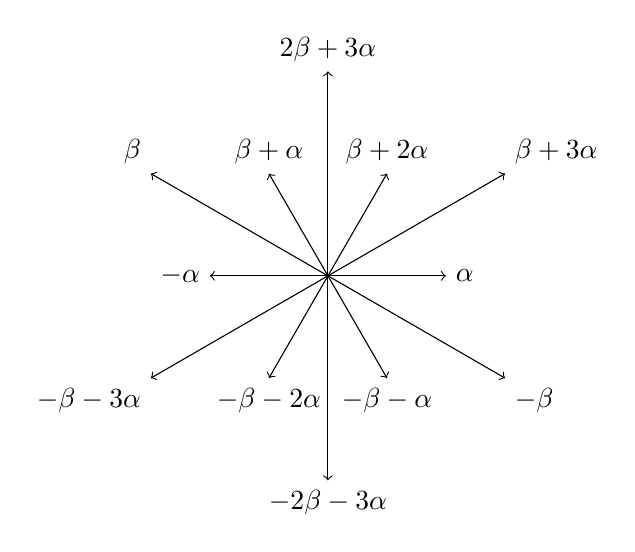
\begin{tikzpicture}[scale = 1.5]
    \foreach \ang in {60, 120, ..., 360}{
      \draw[->] (0,0) -- (\ang:1);
      \draw[->] (0,0) -- (\ang + 30 : 1.732); % 1.732 = sqrt(3)
    }
    \node[anchor=west]        at (0:1)        {$\alpha$};
    \node[anchor=south west]  at (30:1.732)   {$\beta + 3 \alpha$};
    \node[anchor=south]       at (60:1)       {$\beta + 2 \alpha$};
    \node[anchor=south]       at (90:1.732)   {$2 \beta + 3 \alpha$};
    \node[anchor=south]       at (120:1)      {$\beta + \alpha$};
    \node[anchor=south east]  at (150:1.732)  {$\beta$};
    \node[anchor=east]        at (180:1)      {$-\alpha$};
    \node[anchor=north east]  at (210:1.732)  {$-\beta - 3 \alpha$};
    \node[anchor=north]       at (240:1)      {$-\beta - 2 \alpha$};
    \node[anchor=north]       at (270:1.732)  {$-2 \beta - 3 \alpha$};
    \node[anchor=north]       at (300:1)      {$-\beta - \alpha$};
    \node[anchor=north west]  at (330:1.732)  {$-\beta$};
  \end{tikzpicture}
  \end{center}
  This root system is crystallographic and can hence be understood as a root system over an arbitrary field~$\kf$.
  To see how this resulting~{\rootsystem{$\kf$}} looks like we choose a basis~$\alpha$,~$\beta$ of~$\Real^2$ as indicated above.
  Then every root is a linear combination of~$\alpha$,~$\beta$ with integer coefficients.
  Applying the above constructions (restriction of scalars~$\Real \to \Rational$ followed by extension of scalars~$\Rational \to \kf$) we arrive at a~{\rootsystem{$\kf$}}~$R$ of rank~$2$ in a vector space~$V$ with basis~$\alpha$,~$\beta$ such that
  \[
    R
    =
    \Bigl\{
      \pm \alpha,
      \pm (\beta + 3 \alpha),
      \pm (\beta + 2 \alpha),
      \pm (2 \beta + 3 \alpha),
      \pm (\beta + \alpha),
      \pm \beta
    \Bigr\} \,.
  \]
  The reflection~$s_{\gamma}$ for~$\gamma \in R$ is in the picture given by the orthogonal reflection at the line that is orthogonal to~$\gamma$.
  With respect to the basis~$\alpha$,~$\beta$ of~$V$ these reflections can be expressed by the following matrices:
  \begin{alignat*}{3}
    s_\alpha
    &\equiv
    \begin{bmatrix*}[r]
      -1  & 3 \\
       0  & 1
    \end{bmatrix*} \,,
    &
    \quad
    s_{\beta + 3 \alpha}
    &\equiv
    \begin{bmatrix*}[r]
      -2 & 3 \\
      -1 & 2
    \end{bmatrix*} \,,
    &
    \quad
    s_{\beta + 2 \alpha}
    &\equiv
    \begin{bmatrix*}[r]
      -1  & 0 \\
      -1  & 1
    \end{bmatrix*} \,,
  \\
    s_{2 \beta + 3 \alpha}
    &\equiv
    \begin{bmatrix*}[r]
      1 & -3 \\
      0 & -1
    \end{bmatrix*} \,,
    &
    \quad
    s_{\beta + \alpha}
    &\equiv
    \begin{bmatrix*}[r]
      2 & -3 \\
      1 & -2 
    \end{bmatrix*} \,,
    &
    \quad
    s_\beta
    &\equiv
    \begin{bmatrix*}[r]
      1 &  0 \\
      1 & -1
    \end{bmatrix*} \,.
  \end{alignat*}
  We denote this root system by~$\rootG_2$.
  
  To determine the Weyl group of~$\rootG_2$ we may, by the above discussions, consider the starting case~$\kf = \Real$ with~$s_\gamma$ being the orthogonal reflection as explained above.
  We may draw the lines at which we reflect together with a hexagon into the following picture:
  \begin{center}
  \begin{tikzpicture}[scale = 1.5]
    \foreach \ang in {30, 60, ..., 360}{
      \draw[-, dashed] (0,0) -- (\ang:2);
    }
    \draw (0:1.5) -- (60:1.5) -- (120:1.5) -- (180:1.5) -- (240:1.5) -- (300:1.5) -- cycle;
  \end{tikzpicture}
  \end{center}
  We see from this picture that the Weyl group~$\Weyl(\rootG_2)$, which is generated by the reflection at these lines, is precisely the dihedral group of the hexagon,~$\dihedral_6$.
\end{example}





\subsection{Coroots and Duality of Root Systems}


\begin{definition}
  Let~$R$ be a root system in a~{\vectorspace{$\kf$}}~$V$.
  Let~$W$ be another~{\vectorspace{$\kf$}} and let~$\pair{-,-} \colon V \times W \to \kf$ be a non-degenerate bilinear form.
  For every root~$\alpha \in R$ there exists by \cref{reflections using duality} a unique element~$\check{\alpha} \in W$ such that the reflection~$s_\alpha$ is given by~$s_\alpha(v) = v - \pair{v, \check{\alpha}} \alpha$ for every~$v \in V$.
  The element~$\check{\alpha}$ is the \defemph{coroot} associated to~$\alpha$ (with respect to the pairing~$\pair{-,-}$).
  The set of coroots is denoted by~$\check{R} = \{\check{\alpha} \suchthat \alpha \in R\}$.
  (This is a subset of~$W$.)
\end{definition}


\begin{remark}
  If~$\alpha, \beta \in R$ are proportional roots, i.e.\ if~$\beta = \lambda \alpha$ for some scalar~$\lambda$ (necessarily nonzero) then~$s_\alpha = s_\beta$ and then also~$\check{\beta} = \lambda^{-1} \check{\alpha}$.
  In particular~$\check{(-\alpha)} = -\check{\alpha}$.
  But if~$\alpha, \beta \in R$ are two roots whose sum~$\alpha + \beta$ is again a root, then in general~$\check{(\alpha + \beta)} = \check{\alpha} + \check{\beta}$.
\end{remark}


% TODO: Give a counterexample that show that check does not have to be compatible with sums.


\begin{proposition}
  \label{dual root system}
  Let~$R$ be a root system in a~{\vectorspace{$\kf$}}~$V$ and let~$\pair{-,-} \colon V \times W \to \kf$ be a non-degenerate bilinear form.
  \begin{enumerate}
    \item
      \label{coroots are a root system}
      The set of coroots~$\check{R}$ is a root system in~$W$.
    \item
      \label{description of dual reflections}
      For every root~$\alpha \in R$ the reflections~$s_{\check{\alpha}}$ and~$s_\alpha$ are related by~$s_{\check{\alpha}} = s_\alpha^*$, and the reflection~$s_{\check{\alpha}}$ is given on coroots by~$s_{\check{\alpha}}(\check{\beta}) = \check{s_\alpha(\beta)}$ for every~$\beta \in R$.
    \item
      \label{antiisomorphism of weyl groups}
      The algebra anti-isomorphism~$\End(V) \to \End(W)$ given by~$f \mapsto f^*$ restricts to a group anti-isomorphism~$\Weyl(R) \to \Weyl(\check{R})$.
  \end{enumerate}
\end{proposition}


\begin{proof}
  It follows for every root~$\alpha \in R$ from~$\pair{\alpha, \check{\alpha}} = 2$ that~$\check{\alpha} \neq 0$ whence~$0 \notin \check{R}$.
  Suppose that~$W$ were not spanned by~$\check{R}$.
  Then~$\gen{\check{R}}_{\kf}$ is a proper subspace of~$W$ whence its orthogonal~$\gen{\check{R}}_{\kf}^\perp$ is a nonzero linear subspace of~$V$.
  There hence exists some nonzero vector~$v \in V$ with~$\pair{v, \check{\alpha}} = 0$ for every~$\alpha \in R$.
  This then means that the nonzero vector~$v$ is fixed by every reflection~$s_\alpha$ with~$\alpha \in R$, and hence fixed by every element of the Weyl group~$\Weyl(R)$.
  But this contradicts \cref{weyl groups fixes no line}.
  We therefore find that~$W$ is spanned by~$\check{R}$.
  
  To finish proving part~\ref*{coroots are a root system} and to prove part~\ref*{description of dual reflections} we need to show that for every root~$\alpha \in R$ the linear map~$s_\alpha^* \colon W \to W$ is a reflection with~$s_\alpha^*(\check{\alpha}) = -\check{\alpha}$,~$s_\alpha^*(\check{R}) \subseteq \check{R}$ and~$s_\alpha^*(\check{\beta}) = \check{s_\alpha(\beta)}$.
  That~$s_\alpha^*$ is again a reflection follows from part~\ref*{dual reflections} of \cref{properties of reflections}.
  The next two conditions follow from the last condition~$s_\alpha^*(\check{\beta}) = \check{s_\alpha(\beta)}$ because~$\check{(-\alpha)} = -\check{\alpha}$ and~$\check{s_\alpha(\beta)} \in R$.
  
  For this last condition we observe that
  \begin{align}
    s_{s_\alpha(\beta)}
    &=
    s_\alpha \circ s_\beta \circ s_\alpha^{-1}
    \label{pulling apart}
    \\
    &=
    s_\alpha \circ s_{\beta, \check{\beta}} \circ s_\alpha^{-1}
    \notag
    \\
    &=
    s_{s_\alpha(\beta), s_\alpha^{-*}(\check{\beta})}
    \label{pulling together again}
    \\
    &=
    s_{s_\alpha(\beta), s_{\check{\alpha}}(\check{\beta})}
    \label{simplifying index}
  \end{align}
  The equality~\eqref{pulling apart} follows from \cref{reflection of conjugated root}, equality~\eqref{pulling together again} follows from part~\ref*{conjugation of reflection} of \cref{properties of reflections}, and equality~\eqref{simplifying index} follows from part~\ref*{dual reflections} of \cref{properties of reflections} because
  \[
    s_\alpha^{-*}(\check{\beta})
    =
    (s_\alpha^{-1})^*(\check{\beta})
    =
    s_\alpha^*(\check{\beta})
    =
    s_{\check{\alpha}}(\check{\beta}) \,.
  \]
  The above equality~$s_{s_\alpha(\beta)} = s_{s_\alpha(\beta), s_{\check{\alpha}}(\check{\beta})}$ shows that~$s_{\check{\alpha}}(\check{\beta})$ satisfies the defining property of the coroot~$\check{s_\alpha(\beta)}$.
  
  Part~\ref*{antiisomorphism of weyl groups} follows from part~\ref*{description of dual reflections} because the given anti-isomorphism of~{\algebras{$\kf$}}~$\End(V) \to \End(W)$ restricts to an anti-isomorphism of groups~$\GL(V) \to \GL(W)$ which maps the generators~$s_\alpha$ of the Weyl group~$\Weyl(R)$ (with~$\alpha \in R$) onto the generators~$s_\alpha^* = s_{\check{\alpha}}$ of the Weyl group~$\Weyl(\check{R})$.
\end{proof}


\begin{lemma}
  \label{double duality of root systems}
  Let~$R$ be a root system in a~{\vectorspace{$\kf$}}~$V$.
  Let~$W$ be another~{\vectorspace{$\kf$}} and let~$\pair{-,-} \colon V \times W \to \kf$ be a non-degenerate bilinear form.
  For every root~$\alpha \in R$ let~$\dcheck{\alpha} \in V$ be the coroot of~$\check{\alpha} \in \check{R}$ with respect to~$\pair{-,-}$.%
  \footnote{Strictly speaking we do not use~$\pair{-,-}$ to go from~$\check{\alpha}$ to~$\dcheck{\alpha}$ but instead the twisted version of~$\pair{-,-}$ given by the composition~$W \times V \xto{\text{swap}} V \times W \xto{\pair{-,-}} \kf$.}
  Then~$\dcheck{\alpha} = \alpha$ and overall~$\dcheck{R} = R$.
\end{lemma}


\begin{proof}
  Let~$\alpha \in R$ be any root.
  For the associated coroot~$\check{\alpha}$ its reflection~$s_{\check{\alpha}}$ is according to \cref{dual root system} given by~$s_{\check{\alpha}} = s_\alpha^*$.
  The reflection fo the associated double coroot~$\dcheck{\alpha}$ is hence given by~$s_{\dcheck{\alpha}} = s_{\check{\alpha}}^* = s_\alpha^{**} = s_\alpha$.
  It follows from part~\ref*{dual reflections} of \cref{properties of reflections} that the double coroot~$\dcheck{\alpha}$, i.e.\ the unique element~$\dcheck{\alpha} \in V$ with~$s_{\check{\alpha}}(w) = w - \pair{\dcheck{\alpha}, w} \check{\alpha}$ for every~$w \in W$, is given by~$\alpha$ itself.
  Whence~$\dcheck{\alpha} = \alpha$.
\end{proof}


\begin{corollary}
  \label{root to dual root is bijective}
  Let~$R$ be a root system in a~{\vectorspace{$\kf$}}~$V$.
  Let~$W$ be another~{\vectorspace{$\kf$}} and let~$\pair{-,-} \colon V \times W \to \kf$ be a non-degenerate bilinear form.
  Then the map~$R \to \check{R}$ given by~$\alpha \mapsto \check{\alpha}$ is a bijection with inverse given by~$\check{\alpha} \mapsto \dcheck{\alpha} = \alpha$.
  \qed
\end{corollary}


\begin{lemma}
  \label{uniqueness of dual}
  Let~$R$ be a root system in a~{\vectorspace{$\kf$}}~$V$.
  Let~$W_1$ and~$W_2$ be two~{\vectorspaces{$\kf$}} with non-degenerate bilinear forms~$\pair{-,-}_1 \colon V \times W_1 \to \kf$ and~$\pair{-,-}_2 \colon V \times W_2 \to \kf$.
  Let~$\check{R_1}$ and~$\check{R_2}$ be the resulting root systems of coroots in~$W_1$ and~$W_2$.
  Let~$f \colon W_1 \to W_2$ be the unique linear map with
  \begin{equation}
    \label{defining equation for isomorphism of duals}
    \pair{v, w_1}
    =
    \pair{v, \spacing f(w_1)}
  \end{equation}
  for all~$v \in V$ and~$w_1 \in W_1$.
  Then~$f$ is an isomorphism of root systems~$(\check{R_1}, W_1) \to (\check{R_2}, W_2)$.
\end{lemma}


\begin{proof}
  The non-degenerate bilinear forms~$\pair{-,-}_1$ and~$\pair{-,-}_2$ correspond to isomorphisms of vector spaces~$\varphi_1 \colon W_1 \to V^*$ and~$\varphi_2 \colon W_2 \to V^*$ given by~$\varphi_1(w_1) = \pair{-, w_1}_1$ and~$\varphi_2(w_2) = \pair{-, w_2}_2$.
  The proposed linear map~$f \colon W_1 \to W_2$ is precisely the composition~$f = \varphi_2^{-1} \circ \varphi_1$.
  It is is particular an isomorphism of vector spaces.
  It follows from~\eqref{defining equation for isomorphism of duals} that~$f(\check{\alpha}) = \check{\alpha}$ for every~$\alpha \in R$.
  It follows from \cref{root to dual root is bijective} that the linear isomorphism~$f$ maps the root system~$\check{R_1}$ bijectively into the root system~$\check{R_2}$ and is therefore an isomorphism of root systems as asserted.
\end{proof}


\begin{definition}
  Let~$R$ be a root system in a~{\vectorspace{$\kf$}}~$V$.
  Let~$W$ be another vector space and let~$\pair{-,-} \colon V \times W \to \kf$ be a non-degenerate bilinear form.
  The root system~$\check{R}$ in~$W$ is the \defemph{dual \textup(root system\textup)} of~$R$.
\end{definition}


\begin{remark}
  Let~$R$ be a root system in a~{\vectorspace{$\kf$}}~$V$.
  \begin{enumerate}
    \item
      \Cref{uniqueness of dual} shows that the dual of the root system~$R$ does up to (sensible) isomorphism not depend on the choice of non-degenerate bilinear form~$\pair{-,-}$.
      
      As a consequence of this we will often talk about the coroots~$\check{\alpha}$ for~$\alpha \in R$ without specifying the choice of non-degenerate bilinear form~$\pair{-,-}$.
    \item
      Many references define the dual of a root system~$R$ only for a specific choice of non-degenerate bilinear form~$\pair{-,-} \colon V \times W \to \kf$.
      As an example, in \cite[18]{tauvel_yu} and in the lecture (which these notes are based on) coroots and the dual root system is only defined for~$W = V^*$ and~$\pair{-,-}$ the standard pairing.
    \item
      \Cref{double duality of root systems} shows that a root system~$R$ and its dual~$\check{R}$ are indeed dual to each other, in the sense that~$\dcheck{R} = R$ and even~$\dcheck{\alpha} = \alpha$ for every roots~$\alpha \in R$.
  \end{enumerate}
\end{remark}


\begin{example}
  \label{explicit coroots for standard root systems}
  We endow the vector space~$\kf^n$ with the standard pairing~$\pair{-,-} \colon \kf^n \times \kf^n \to \kf$ given by~$\pair{x,y} = \sum_{i=1}^n x_i y_i$.
  In the following we will compute explicitely the coroots and dual root systems of the root systems~$\rootA_n$,~$\rootB_n$,~$\rootC_n$ and~$\rootD_n$.
  \begin{enumerate}
    \item
      We begin with the root system~$\rootB_n$ in~$\kf^n$.
      Recall that
      \[
        \rootB_n
        =
        \{
          \pm e_i
        \suchthat
          i = 1, \dotsc, n
        \}
        \cup
        \{
          \pm e_i \pm e_j
        \suchthat
          1 \leq i \neq j \leq n
        \} \,.
      \]
      By using the explicit descriptions of the reflections~$s_\alpha$ for~$\alpha \in \rootB_n$ we can calculate the coroots with respect to~$\pair{-,-}$.
      \begin{itemize}
        \item
          The reflection~$s_{e_i}$ is given by mapping~$e_i \mapsto -e_i$ and~$e_j \mapsto e_j$ for~$j \neq i$.
          The reflection~$s_{e_i}$ is therefore given by
          \[
            s_{e_i}(x)
            =
            x - 2 x_i e_i
            =
            x - \pair{x, 2 e_i} e_i \,.
          \]
          This shows that~$\check{e_i} = 2 e_i$.
          Then also~$\check{(-e_i)} = -\check{e_i} = -2 e_i$.
        \item
          The reflection~$s_{e_i - e_j}$ is on standard basis vectors given by
          \[
            e_i \mapsto e_j \,,
            \quad
            e_j \mapsto e_i \,,
            \quad
            e_k \mapsto e_k \,,
          \]
          where~$k \neq i,j$.
          This means that
          \[
            e_i
            \mapsto
            e_i - 1 \cdot (e_i - e_j) \,,
            \quad
            e_j
            \mapsto
            e_j - (-1) \cdot (e_i - e_j) \,,
            \quad
            e_k
            \mapsto
            e_k - 0 \cdot (e_i - e_j) \,.
          \]
          We see from this that the linear functional~$\pair{-, \check{(e_i - e_j)}} \colon \kf^n \to \kf$ is given on standard basis vectors by
          \[
            e_i \mapsto 1 \,,
            \quad
            e_j \mapsto -1 \,,
            \quad
            e_k
            \mapsto
            0 \,.
          \]
          This means that~$\check{(e_i - e_j)} = e_i - e_j$.
          It also follows that
          \[
            \check{(-e_i + e_j)}
            =
            -\check{(e_i - e_j)}
            =
            -(e_i - e_j)
            =
            -e_i + e_j \,.
          \]
        \item
          We proceed similarly for the coroot~$\check{(e_i + e_j)}$:
          The reflection~$s_{e_i + e_j}$ is on standard basis vectors given by
          \[
            e_i
            \mapsto
            -e_j \,,
            \quad
            e_j
            \mapsto
            -e_i \,,
            \quad
            e_k
            \mapsto
            e_k
          \]
          for~$k \neq i,j$.
          This means that
          \[
            e_i
            \mapsto
            e_i - 1 \cdot (e_i + e_j) \,,
            \quad
            e_j
            \mapsto
            e_j - 1 \cdot (e_i + e_j) \,,
            \quad
            e_k
            \mapsto
            e_k - 0 \cdot (e_i + e_j) \,.
          \]
          The linear functional~$\pair{-, \check{(e_i + e_j)}} \colon \kf^n \to \kf$ is therefore given by
          \[
            e_i
            \mapsto
            1 \,,
            \quad
            e_j
            \mapsto
            1 \,,
            \quad
            e_k
            \mapsto
            0
          \]
          which tells us that~$\check{(e_i + e_j)} = e_i + e_j$.
          Then also
          \[
            \check{(- e_i - e_j)}
            =
            -\check{(e_i + e_j)}
            =
            -(e_i + e_j)
            =
            - e_i - e_j \,.
          \]
      \end{itemize}
      We see that overall
      \[
        \check{\rootB_n}
        =
        \{
          2 e_i
        \suchthat
          i = 1, \dotsc, n
        \}
        \cup
        \{
          \pm e_i \pm e_j
        \suchthat
          1 \leq i \neq j \leq n
        \} \,.
      \]
      This is precisely the root system~$\rootC_n$.
      We have hence shown that~$\check{\rootB_n} = \rootC_n$.
    \item
      We now also find that
      \[
        \check{\rootC_n}
        =
        \dcheck{\rootB_n}
        =
        \rootB_n \,.
      \]
      More precisely,~$\check{(2 e_i)} = e_i$ for every~$i = 1, \dotsc, n$ and~$\check{(\pm e_i \pm e_j)} = \pm e_i \pm e_j$ for all~$1 \leq i \neq j \leq n$.
    \item
      Recall that the root system~$\rootD_n$ is given by
      \[
        \rootD_n
        =
        \{
          \pm e_i \pm e_j
        \suchthat
          1 \leq i \neq j \leq n \,.
        \}
      \]
      We can reuse the above calculations to find that~$\check{(\pm e_i \pm e_j)} = \pm e_i \pm e_j$ for all~$1 \leq i \neq j \leq n$.
      We hence find that~$\check{\rootD_n} = \rootD_n$.
    \item
      The root system~$\rootA_n$ is given by
      \[
        \rootA_n
        =
        \{
          e_i - e_j
        \suchthat
          1 \leq i \neq \leq j \leq n
        \} \,,
      \]
      and it is a root system in the vector space
      \[
        V
        =
        \{
          (x_1, \dotsc, x_n) \in \kf^n
        \suchthat
          x_1 + \dotsb + x_n = 0
        \} \,.
      \]
      The restriction of the standard pairing~$\pair{-,-}$ to the linear subspace~$V$ of~$\kf^n$ is again non-degenerate since the orthogonal of~$V$ is given by~$V^\perp = \gen{(1, \dotsc, 1)}_{\kf}$ and thus~$\kf^n = V \oplus V^\perp$.
      We denote the restriction of~$\pair{-,-}$ to~$V$ again by~$\pair{-,-}$.
      
      The reflection~$s_{e_i - e_j}$ is the restriction of the reflection~$s_{ij} \colon \kf^n \to \kf^n$ given by
      \[
        e_i
        \mapsto
        e_j \,,
        \quad
        e_j
        \mapsto
        e_i \,,
        \quad
        e_k
        \mapsto
        e_k
      \]
      for~$k \neq i,j$.
      We have seen in the previous calculations that the reflections~$s_{ij}$ are given by
      \[
        s_{ij}(x)
        =
        x - \pair{x, e_i - e_j} (e_i - e_j)
      \]
      for every~$x \in \kf^n$.
      For the reflections~$s_{e_i - e_j}$ the same formula holds (as they are restrictions of the reflections~$s_{ij}$) and we hence find that~$\check{(e_i - e_j)} = e_i - e_j$.
      This shows in particular that~$\check{\rootA_n} = \rootA_n$.0
  \end{enumerate}
\end{example}


\begin{lemma}
  \label{formula for orthogonal coroots}
  Let~$R$ be a root system in a~{\vectorspace{$\kf$}} and let~$\inner{-,-} \colon V \times V \to \kf$ be a non-degenerate symmetric bilinear form.
  Suppose that for every root~$\alpha \in R$ the reflection~$s_\alpha$ is an isometry with respect to~$\inner{-,-}$. 
  Then~$\inner{\alpha, \alpha} \neq 0$ for every root~$\alpha \in R$, and the associated coroot is given by
  \[
    \check{\alpha}
    =
    \frac{2 \alpha}{\inner{\alpha, \alpha}} \,.
  \]
\end{lemma}


\begin{proof}
  
  It follows from \cref{orthogonal reflections are orthogonal reflections} that~$\inner{\alpha, \alpha} \neq 0$ and that the reflection~$s_\alpha$ is given by
  \[
    s_\alpha(v)
    =
    v - 2 \frac{\inner{v,\alpha}}{\inner{\alpha, \alpha}} \alpha
  \]
  for every~$v \in V$.
  We may rewrite this expression as
  \[
    s_\alpha(v)
    =
    v - \inner*{v, \frac{2 \alpha}{\inner{\alpha, \alpha}} } \alpha \,,
  \]
  which gives the asserted form of~$\check{\alpha}$.
\end{proof}


\begin{examples}
  Let again~$\inner{-,-}$ be the standard symmetric bilinear form on~$\kf^n$, still given by~$\inner{x,y} = \sum_{i=1}^n x_i y_i$.
  Let~$V = \{ (x_1, \dotsc, x_n) \in \kf^n \suchthat x_1 + \dotsb + x_n = 0 \}$ be the linear subspace of~$\kf^n$ in which~$\rootA_n$ is a root system.
  We denote the restriction of~$\inner{-,-}$ to~$V$ again by~$\inner{-,-}$.
  
  We have seen in \cref{standard root systems have isometric reflections} that for the root systems~$\rootA_n$,~$\rootB_n$,~$\rootC_n$ and~$\rootD_n$ the reflections~$s_\alpha$, for~$\alpha$ some root, are isometries with respect to~$\inner{-,-}$..
  We can therefore apply \cref{formula for orthogonal coroots} to calculate the coroots a second time:  
  We have
  \[
    \inner{\pm e_i,  \pm e_i}
    =
    1 \,,
    \quad
    \inner{\pm 2 e_i, \pm 2 e_i}
    =
    4 \,,
    \quad
    \inner{\pm e_i \pm e_j, \pm e_i \pm e_j}
    =
    2
  \]
  where the signs in the first argument are choosen arbitrary but the signs in the second argument are as in the first argument.
  It follows that
  \begin{align*}
    \check{(\pm e_i)}
    &=
    \frac{2}{\inner{\pm e_i,  \pm e_i}}
    \cdot
    (\pm e_i)
    =
    \frac{2}{1}
    \cdot
    (\pm e_i)
    =
    \pm 2 e_i \,,
    \\[0.5em]
    \check{(\pm 2 e_i)}
    &=
    \frac{2}{\inner{\pm 2 e_i,  \pm 2 e_i}}
    \cdot
    (\pm 2 e_i)
    =
    \frac{2}{4}
    \cdot
    (\pm 2 e_i)
     =
    \pm e_i \,,
    \\[0.5em]
    \check{(\pm e_i \pm e_j)}
    &=
    \frac{2}{\inner{\pm e_i \pm e_j,  \pm e_i \pm e_j}}
    \cdot
    (\pm e_i \pm e_j)
    =
    \frac{2}{2}
    \cdot
    (\pm e_i \pm e_j)
    =
    \pm e_i \pm e_j \,.
  \end{align*}
  These are indeed the same results as in \cref{explicit coroots for standard root systems}.
\end{examples}


% TODO: G2 selfdual; how to prove?


\begin{definition}
  Let~$R$ be a root system in a~{\vectorspace{$\kf$}}.
  By \cref{reflected vector is a linear combination} there exists for any two roots~$\alpha, \beta \in R$ a scalar~$c_{\alpha \beta} \in \kf$ with~$s_{\beta}(\alpha) = \alpha - c_{\alpha \beta} \beta$.
  The numbers~$c_{\alpha \beta}$ are the \defemph{Cartan numbers}.
\end{definition}


\begin{lemma}
  \label{properties via cartan numbers}
  \leavevmode
  \begin{enumerate}
    \item
      \label{crystallographic via cartan numbers}
      A root system~$R$ is crystallographic if and only if~$c_{\alpha \beta} \in \Integer$ for any two roots~$\alpha, \beta \in R$.
    \item
      Let~$\Lf/\kf$ be a field extension and let~$R$ be an~{\rootsystem{$\Lf$}}.
      Then~$R$ is definable over~$\kf$ if and only if~$c_{\alpha \beta} \in \kf$ for any two roots~$\alpha, \beta \in R$.
    \qedhere
  \end{enumerate}
\end{lemma}


\begin{remark}
  For the crystallographic root system~$R$ the Cartan numbers are also known as \defemph{Cartan integers}.
\end{remark}


\begin{lemma}
  \label{cartan numbers via coroots}
  Let~$R$ be a root system in a~{\vectorspace{$\kf$}}~$V$.
  The Cartan numbers of~$R$ are given by~$c_{\alpha \beta} = \pair{\alpha, \check{\beta}}$ for any two roots~$\alpha, \beta \in R$.
\end{lemma}


\begin{proof}
  We have~$s_\beta(\alpha) = \alpha - \pair{\alpha, \check{\beta}} \beta$ whence~$\pair{\alpha, \check{\beta}}$ satisfies the defining propery of~$c_{\alpha \beta}$.
\end{proof}


\begin{corollary}
  \leavevmode
  \begin{enumerate}
    \item
      A root system~$R$ is crystallographic if and only if~$\pair{\alpha, \check{\beta}} \in \Integer$ for any two roots~$\alpha, \beta \in R$.
    \item
      Let~$\Lf/\kf$ be a field extension.
      An~{\rootsystem{$\Lf$}}~$R$ is definable over~$\kf$ if and only if~$\pair{\alpha, \check{\beta}} \in \kf$ for any two roots~$\alpha, \beta \in R$.
  \end{enumerate}
\end{corollary}


\begin{proof}
  This is a reformulation of \cref{properties via cartan numbers} via \cref{cartan numbers via coroots}.
\end{proof}


\begin{corollary}
  Let~$R$ be a root system.
  The Cartan numbers for~$R$ and for its dual root system~$\check{R}$ satisfy for two roots~$\alpha, \beta \in R$ the equality
  \[
    c_{\alpha \beta}
    =
    c_{\check{\beta} \check{\alpha}} \,.
  \]
\end{corollary}


\begin{proof}
  Let~$\pair{-,-} \colon V \times W \to \kf$ be a non-degenerate bilinear form.
  Then
  \[
    c_{\alpha \beta}
    =
    \pair{\alpha, \check{\beta}}
    \quad\text{and}\quad
    c_{\check{\beta} \check{\alpha}}
    =
    \pair{\dcheck{\alpha}, \check{\beta}} \,.
  \]
  The assertion follows since~$\dcheck{\alpha} = \alpha$.
\end{proof}


% TODO: Extension and restriction of fields for coroots.


\begin{proposition}
  Let~$\Lf/\kf$ be a field extension.
  \begin{enumerate}
    \item
      Let~$V$ be a root system in a~{\vectorspace{$\kf$}}~$V$ and let~$\pair{-,-} \colon V \times W \to \kf$ be a non-degenerate bilinear form.
      The bilinear form~$\pair{-,-}$ extends uniquely to an~{\bilinear{$\Lf$}} form~$\pair{-,-}_\Lf \colon V_{\Lf} \times W_{\Lf} \to \Lf$.
      This bilinear form is again non-degenerate, and the coroots of the extended root system~$R_{\Lf}$ with respect to~$\pair{-,-}_{\Lf}$ satisfy
      \[
        \check{(1 \tensor \alpha)}
        =
        1 \tensor \check{\alpha}
      \]
      for every~$\alpha \in R$.
      As a consequence~$\check{(R_{\Lf})} = (\check{R})_{\Lf}$.
    \item
      Let~$R$ be a root system in an~{\vectorspace{$\Lf$}}~$V$ and let~$\pair{-,-} \colon V \times W \to \Lf$ be a non-degenerate bilinear form.
      Suppose that the root system~$R$ is definable over~$\kf$.
      Then the dual root system~$\check{R}$ is also definable over~$\kf$.
      The~{\bilinear{$\Lf$}} form~$\pair{-,-}$ restricts to a well-defined~{\bilinear{$\kf$}} form~$\restrict{\pair{-,-}}{\kf} \colon \restrict{V}{\kf} \times \restrict{W}{\kf} \to \kf$.
      This restricted bilinear form is again non-degenerate and the coroot of~$\alpha \in R$ with respect to~$\restrict{\pair{-,-}}{\kf}$ coincides with the coroot with respect to~$\pair{-,-}$.
      In particular~$\check{(\restrict{R}{\kf})} = \restrict{\check{R}}{\kf}$.
  \end{enumerate}
\end{proposition}





\section{Euclidian Root Systems}


\begin{definition}
  A real root system~$(R, V)$ is \defemph{euclidian} if~$V$ is a real inner product space and the reflections~$s_\alpha$ for~$\alpha \in R$ are isometries.
\end{definition}

% TODO: Remark regarding the terminology.





\subsection{Bases and Positive Roots}


\begin{definition}
  Let~$R$ be a root system in a~{\vectorspace{$\kf$}}~$V$.
  \begin{enumerate}
    \item
      A subset~$\Pi \subseteq R$ is a \defemph{positive system} if
      \begin{enumerate}
        \item
          for every root~$\alpha \in R$ precisely one of the two roots~$\alpha$ and~$-\alpha$ is contained in~$R$, and
        \item
          for any two roots~$\beta_1, \beta_2 \in \Pi$ also~$\beta_1 + \beta_2 \in \Pi$.
      \end{enumerate}
      The elements of~$\Pi$ are \defemph{positive roots}, the elements of~$-\Pi$ are \defemph{negative roots}.
      An positive root~$\alpha \in \Pi$ is \defemph{decomposable} if it can be written as~$\alpha = \beta_1 + \beta_2$ for two positive roots~$\beta_1, \beta_2 \in \Pi$.
      Otherwise it is \defemph{indecomposable}.
    \item
      A subset~$\Delta \subseteq R$ is a \defemph{basis} of~$R$ if 
      \begin{enumerate}
        \item
          $\Delta$ is a vector space basis of~$V$, and
        \item
          for every root~$\beta \in R$ the linear combination~$\beta = \sum_{\alpha \in \Delta} k_\alpha \alpha$ satisfies~$k_\alpha \in \Integer_{\geq 0}$ for every~$\alpha \in \Delta$ or~$k_\alpha \in \Integer_{\leq 0}$ for every~$\alpha \in \Delta$.
      \end{enumerate}
      The elements of~$\Delta$ are~\defemph{simple roots}.
  \end{enumerate}
\end{definition}


\begin{proposition}
  Let~$R$ be a reduced crystallographic root system.
  \begin{enumerate}
    \item
      Let~$\Delta$ be a basis of~$R$.
      Then
      \[
        \Pi
        =
        \left\{
          \beta \in R
        \suchthat*
          \text{$\beta = \sum_{\alpha \in \Delta} k_\alpha \alpha$ with~$\alpha \in \Integer_{\geq 0}$ for every~$\alpha \in \Delta$}
        \right\} \,.
      \]
      is a positive system for~$R$.
    \item
      Let~$\Pi$ be a positive system for~$R$.
      Then
      \[
        \Delta
        =
        \{
          \text{$\alpha \in \Pi$ is indecomposable}
        \}
      \]
      is a basis of~$R$.
    \item
      The above constructions give a {\onetoone} correspondence
      \[
        \{
          \text{positive systems~$\Pi \subseteq R$}
        \}
        \longonetoone
        \{
          \text{bases~$\Delta \subseteq R$}
        \} \,.
      \]
  \end{enumerate}
\end{proposition}


\begin{proof}
  We will show this later.
\end{proof}








% \section{Coroots}
% 
% \begin{lemma}
%   \label{properties of coroots}
%   Let~$R$ be a root system in a~{\vectorspace{$\kf$}}~$V$.
%   \begin{enumerate}
%     \item
%       If~$\alpha \in R$ is a root and~$\lambda \neq 0$ such that~$\lambda \alpha$ is again a root then~$\check{(\lambda \alpha)} = \lambda^{-1} \check{\alpha}$.
%     \item
%       For all~$\alpha, \beta \in R$,~$\check{s_\alpha(\beta)} = s_{\check{\alpha}, \alpha}(\check{\beta})$.
%   \end{enumerate}
% \end{lemma}
% 
% 
% \begin{proof}
%   \leavevmode
%   \begin{enumerate}
%     \item
%       We have~$\pair{\lambda \alpha, \lambda^{-1} \check{\alpha}} = \pair{\alpha, \check{\alpha}} = 2$ whence the reflection~$s_{\lambda \alpha, \spacing \lambda^{-1} \alpha}$ is well-defined.
%       It follows from part~\ref*{uniqueness of reflection parametrization} of \cref{regarding general reflections} that~$s_{\lambda \alpha, \spacing \lambda^{-1} \check{\alpha}} = s_{\alpha, \check{\alpha}}$, which shows that~$s_{\lambda \alpha, \spacing \lambda^{-1} \check{\alpha}}$ leaves~$R$ invariant.
%       Together this shows that~$\lambda^{-1} \check{\alpha}$ satisfies the defining properties of~$\check{(\lambda \alpha)}$.
%     \item
%       We have
%       \[
%         \pair{s_\alpha(\beta), s_{\check{\alpha}, \alpha}(\check{\beta})}
%         =
%         \pair{s_\alpha(\beta), s_\alpha^*(\check{\beta})}
%         =
%         \pair{s_\alpha^2(\beta), \check{\beta}}
%         =
%         \pair{\beta, \check{\beta}}
%         =
%         2
%       \]
%       where we use that~$s_{\check{\alpha}, \alpha}= s_{\alpha, \check{\alpha}}^* = s_\alpha^*$ by \cref{properties of reflections}.
%       The reflection~$s_{[s_\alpha(\beta)], [s_{\check{\alpha}, \alpha}(\check{\beta})]}$ is therefore well-defined.%
%       \footnote{The brackets are only here for better readability and have no meaning on their own.}
%       We also see from \cref{properties of reflections} that
%       \[
%         s_{[s_\alpha(\beta)], [s_{\check{\alpha}, \alpha}(\check{\beta})]}
%         =
%         s_{[s_\alpha(\beta)], [s_\alpha^*(\check{\beta})]}
%         =
%         s_\alpha \circ s_\beta \circ s_\alpha^{-1} 
%         =
%         s_\alpha \circ s_\beta \circ s_\alpha \,.
%       \]
%       We see from this that the reflection~$s_{[s_\alpha(\beta)], [s_{\check{\alpha}, \alpha}(\check{\beta})]}$ leaves~$R$ invariant.
%       This shows that~$s_{\check{\alpha}, \alpha}(\check{\beta})$ satisfies the defining property of the coroot~$\check{s_\alpha(\beta)}$.
%     \qedhere
%   \end{enumerate}
% \end{proof}
% 
% 
% \begin{theorem}
%   \label{dual root system}
%   If~$R$ is a root system in a~{\vectorspace{$\kf$}}~$V$ then the set of coroots~$\check{R}$ is a root system in~$V^*$.
%   For every~$\alpha \in R$ the coroot of~$\check{\alpha}$, i.e.\ the element~$\dcheck*{\alpha} \in V^{**}$, is given by evaluation at~$\alpha$.
%   If~$R$ is reduced or crystallographic then the same holds for~$\check{R}$.
% \end{theorem}
% 
% 
% \begin{proof}
%   If~$0 \in \check{R}$ then~$\check{\alpha} = 0$ for some~$\alpha \in R$, which would contradict~$\pair{\alpha, \check{\alpha}} = 2$.
%   Thus~$0 \notin \check{R}$.
%   
%   The set of coroots~$\check{R}$ spans~$V^*$:
%   Otherwise the the span of~$\check{R}$ would a proper linear subspace of~$V^*$.
%   Then there would exists some nonzero~$v \in V$ with~$\pair{v, \varphi} = 0$ for every~$\varphi$ contained in this span.
%   Then in particular~$\pair{v, \check{\alpha}} = 0$ for every~$\alpha \in R$ and thus~$s_\alpha(v) = v$ for every~$\alpha \in R$.
%   Then~$w(v) = v$ for every~$w \in \Weyl(R)$, which would contradicts \cref{weyl group fixes no vector}.
%   Thus~$\check{R}$ spans~$V^*$
%   
%   For every~$\alpha \in R$ the proposed coroot of~$\check{\alpha} \in \check{R}$ is the element~$\dcheck*{\alpha} \in V^{**}$ given by evaluation at~$\alpha$.
%   Indeed,~$\pair{\check{\alpha}, \dcheck{\alpha}} = \pair{\alpha, \check{\alpha}} = 2$ and for every~$\beta \in R$,
%   \[
%     s_{\check{\alpha}, \dcheck{\alpha}}(\check{\beta})
%     =
%     s_{\check{\alpha}, \alpha}(\check{\beta})
%     =
%     \check{s(\beta)}
%     \in
%     \check{R}
%   \]
%   by \cref{properties of coroots}.
%   This shows that~$\check{R}$ is indeed a root system, with the coroot~$\dcheck*{\alpha} \in V^{**}$ of~$\check{\alpha}$ given by evaluation at~$\alpha$.
%   
%   Suppose that~$R$ is reduced, and that for some~$\alpha \in R$ some multiple~$\lambda \check{\alpha}$ is contained in~$R$.
%   Note that necessarily~$\lambda \neq 0$ since~$0 \notin \check{R}$.
%   Then also~$\lambda^{-1} \dcheck{\alpha} = \check{(\lambda\check{\alpha})} \in \dcheck{R}$ by \cref{properties of coroots}.
%   We know that under the natural isomorphism~$V \cong V^{**}$ the root system~$R$ corresponds to~$\dcheck{R}$;
%   more precisely,~$\alpha$ corresponds to~$\dcheck{\alpha}$.
%   It hence follows from~$\lambda^{-1} \dcheck*{\alpha} \in \dcheck{R}$ that~$\lambda^{-1} \alpha \in R$.
%   It follows that~$\lambda^{-1} = \pm 1$ and thus~$\lambda = \pm 1$ because~$R$ is reduced.
%   Thus the only multiples of~$\check{\alpha}$ contained in~$\check{R}$ are~$\check{\alpha}$ and~$-\check{\alpha}$, showing that~$\check{R}$ is again reduced.
%   
%   Suppose that~$R$ is crystallographic.
%   Then~$\pair{\check{\alpha}, \dcheck{\beta}} = \pair{\beta, \check{\alpha}} \in \Integer$ for all~$\alpha, \beta \in R$.
%   Thus~$\check{R}$ is again crystallographic.
% \end{proof}
% 
% 
% \begin{remark}
%   If~$R$ is a root system in a~{\vectorspace{$\kf$}}~$V$ then by applying \cref{dual root system} two times we see that not only is~$\check{R}$ is a root system in~$V^*$ but also that~$\dcheck{R}$ is a root system in~$V^{**}$.
%   We then see from \cref{dual root system} that the natural isomorphism~$V \to V^{**}$ is an isomorphism of root systems~$R \to \dcheck{R}$.
%   In this sense the root systems~$R$ and~$\check{R}$ are mutually dual.
% % TODO: Come back to this once root data have been introduced.
%   A consequence of this duality is the following:
% \end{remark}
% 
% 
% \begin{corollary}
%   If~$R$ is a root system then the map~$R \to \check{R}$,~$\alpha \mapsto \check{\alpha}$ is a bijection.
%   \qed
% \end{corollary}
% 
% 
% \begin{corollary}
%   Let~$R$ be a root system in a~{\vectorspace{$\kf$}}~$V$ with decomposition~$R = R_1 \cup \dotsb \cup R_n$.
%   Then~$R = R_1 \times \dotsb \times R_n$ if and only if~$\pair{\alpha, \check{\beta}} = 0$ for all~$\alpha \in R_i$ and~$\beta \in R_j$ with~$i \neq j$.
% \end{corollary}
% 
% 
% \begin{proof}
%   If~$R = R_1 \times \dotsb \times R_n$ then~$\pair{\alpha, \check{\beta}} = 0$ for all~$\alpha \in R_i$ and~$\beta \in R_j$ with~$i \neq j$ by part~\ref*{root summands are orthogonal} of \cref{properties of decompositions}.
%   
%   Suppose now that conversely~$\pair{\alpha, \check{\beta}} = 0$ for all~$\alpha \in R_i$ and~$\beta \in R_j$ with~$i \neq j$.
%   To show that~$R = R_1 \times \dotsb \times R_n$ it sufficies --- thanks to induction --- to consider the case~$n = 2$.
%   
%   Let~$V_i$ be the span of~$R_i$.
%   Then~$V = V_1 + V_2$ because~$R$ spans~$V$.
%   We need to check that~$V_1 \cap V_2 = 0$, as we can then apply \cref{decomposition of root systems}.
%   If~$v \in V_1 \cap V_2$ then it follows from~$v \in V_1$ that~$\pair{v, \check{\beta}} = 0$ for all~$\beta \in R_2$ and it follows from~$v \in V_2$ that~$\pair{v, \check{\beta}} = 0$ for all~$\beta \in R_1$.
%   Therefore~$\pair{v, \check{\beta}} = 0$ for all~$\beta \in R$ and thus~$s_\beta(v) = v$ for every~$\beta \in R$.
%   It follows from \cref{weyl group fixes no vector} that~$v = 0$.
% \end{proof}
% 
% 
% \begin{lemma}
%   Let~$R$ be a root system in a~{\vectorspace{$\kf$}}~$V$.
%   Then the Weyl~groups~$\Weyl(R)$ and~$\Weyl(\check{R})$ are isomorphic via the mapping
%   \[
%     \Weyl(R)
%     \to
%     \Weyl(\check{R}) \,,
%     \quad
%     w
%     \mapsto
%     w^{-*} \,.
%   \]
% \end{lemma}
% 
% 
% \begin{proof}
%   The map~$\End_{\kf}(V) \to \End_{\kf}(V^*)$,~$f \mapsto f^*$ is an algebra anti-isomorphism and thus induces a group anti-isomorphism~$\GL(V) \to \GL(V^*)$,~$f \mapsto f^*$.
%   The Weyl group~$\Weyl(R)$ is generated by the reflections~$s_{\alpha,\check{\alpha}}$ with~$\alpha \in R$ and the Weyl group~$\Weyl(\check{R})$ is generated by the reflections~$s_{\check{\alpha}, \dcheck{\alpha}} = s_{\check{\alpha}, \alpha} = s_{\alpha, \check{\alpha}}^*$ with~$\alpha \in R$.
%   The group anti-isomorphism~$\GL(V) \to \GL(V^*)$ therefore restricts to a group anti-isomorphism~$\Weyl(R) \to \Weyl(\check{R})$,~$w \mapsto w^*$.
%   By composing with the group anti-automorphism~$\Weyl(\check{R}) \to \Weyl(\check{R})$,~$w \mapsto w^{-1}$ we arrive at the claimed the group isomorphism~$\Weyl(R) \to \Weyl(\check{R})$,~$w \mapsto w^{-*}$.
% \end{proof}
% 
% 
% \begin{warning}
%   Even though the root systems~$R$ and~$\check{R}$ have isomorphic Weyl group, the root systems themselves are not necessarily isomorphic.
% \end{warning}




